\chapter{初段ミューオントリガーの性能評価}\label{chapter5}
本章では、第~\ref{chapter4}章で述べた手法を用いて作成した2種類のCW(シミュレーション用のCWと実際の測定用のCW)を用いたトリガーの性能の評価を行う。

\section{機械学習を用いて作成したCWの15段階閾値の評価}
便宜上、本研究の手法で作成した2種類のCWについて、シミュレーション用のCWを$\mathrm{CW_{Simu}}$、実際の測定用のCWを$\mathrm{CW_{Data}}$と呼び、比較対象として2022年度Run-3で使用されたCWを$\mathrm{CW_{2022}}$と呼ぶこととする。

\ref{L1Topo}節で述べたL1 Triggerには、ミューオンの不変質量を指針としたトリガーを持つL1Topoが存在する。しかし、不変質量を計算するときに使用するミューオンの運動量は、L1Muonから送られてくる$p_{\rm{T}}$閾値であるため、L1Muonの$p_{\rm{T}}$閾値の細かさがそのままL1Topoのトリガー性能に影響する。
そこで、Run-3ではL1Muonにおける判定可能な$p_{\rm{T}}$閾値を6段階から15段階に増設することで、より細かい精度での$p_{\rm{T}}$判定を可能とし、L1 Trigger全体としてのトリガー性能の向上を図った。
したがって、本研究で作成するCWにも正確に15段階の$p_{\rm{T}}$判定ができることが要求される。

そこで、全オフライン再構成されたミューオンの内、ある$p_{\rm{T}}$閾値以上のトリガーが発行された割合$\epsilon$を計算し、トリガー効率の算出を行った。また、$\epsilon$をオフライン再構成した$p_{\rm{T}}$の関数として表したTurn-on curveを描き、式~\eqref{equ:fitting}の関数によってフィッティングを行う事で、トリガー性能の評価を行った。
このとき、Tag$\&$Probe法を用いて評価に用いるデータの処理を行う。

\subsubsection{Tag$\&$Probe法}
実際の実験データはトリガーによって選別された粒子の情報のみが保存されているため、そのままのデータを用いてトリガーの性能評価を行うとバイアスがかかる可能性がある。そこで、このバイアスを除く手法としてTag$\&$Probe法を用いる。

Tag$\&$Probe法では、一般的に$Z$ボゾンや$J/\psi$粒子の崩壊で生じた2つのミューオンを使用し評価を行う。崩壊由来の2つのミューオンのうち、片方のミューオン(Tag)が事象選択のトリガーとしてトリガーが発行された場合、もう一方のミューオン(Probe)をトリガー効率の評価に用いる。Probeミューオンに対してトリガーが発行されたかを見ることで、実際の測定でトリガーによって取得されたミューオンというバイアスをなくしてトリガー効率を見積もることができる。

本研究では、内部飛跡検出器とミューオン検出器でそれぞれ独立にオフライン再構成されたZボソン由来のミューオンを用いて評価を行う。1回の衝突事象に対し、2つ以上のミューオン候補が存在するイベントのみを用いる。それらのミューオン候補のうち、任意の2つの電荷が異符号となっているミューオンペアを選び出し、不変質量を再構成する。再構成した不変質量が80 GeV$<M_Z<$100~GeVであることを要求することでZボソン由来のミューオンと判断する。
これらのミューオンのうち、一方をTagミューオン、もう一方をProbeミューオンと定義する。
まず、Tagミューオンがトリガーを発行したかどうかを判定する。Run-2での実験データを解析に使用する際のトリガー判定には、HLTのシングルミューオントリガーである「HLT$\_$mu26$\_$ivarmeduium」を使用する。
ここでトリガー発行の判定を行うために $\Delta R= \sqrt{(\Delta \eta)2 + (\Delta \phi)2}$を定義する。
ここで$\Delta\eta$, $\Delta\phi$はデータに保存されているトリガーを発行した飛跡情報と、オフライン再構成されたTagミューオンの$\eta$方向、$\phi$方向の差分である。
図~\ref{fig:tag_HLT}にTag ミューオンとHLTの$\Delta R$を$p_{\rm{T}}$の関数として表した2次元分布を示す。
本研究では$\Delta R< 0.001$を満たせばTagミューオンがトリガーを発行したとみなす。
TagミューオンがHLTを発行しているとみなされた時、もう一つのミューオンをProbeミューオンとして使用する。Probeミューオンはデータ保存のために発行されたトリガーとは独立なミューオンであるためバイアスの影響はない。

\begin{figure}[htb]
  \centering
  %\rule{8cm}{6cm}
  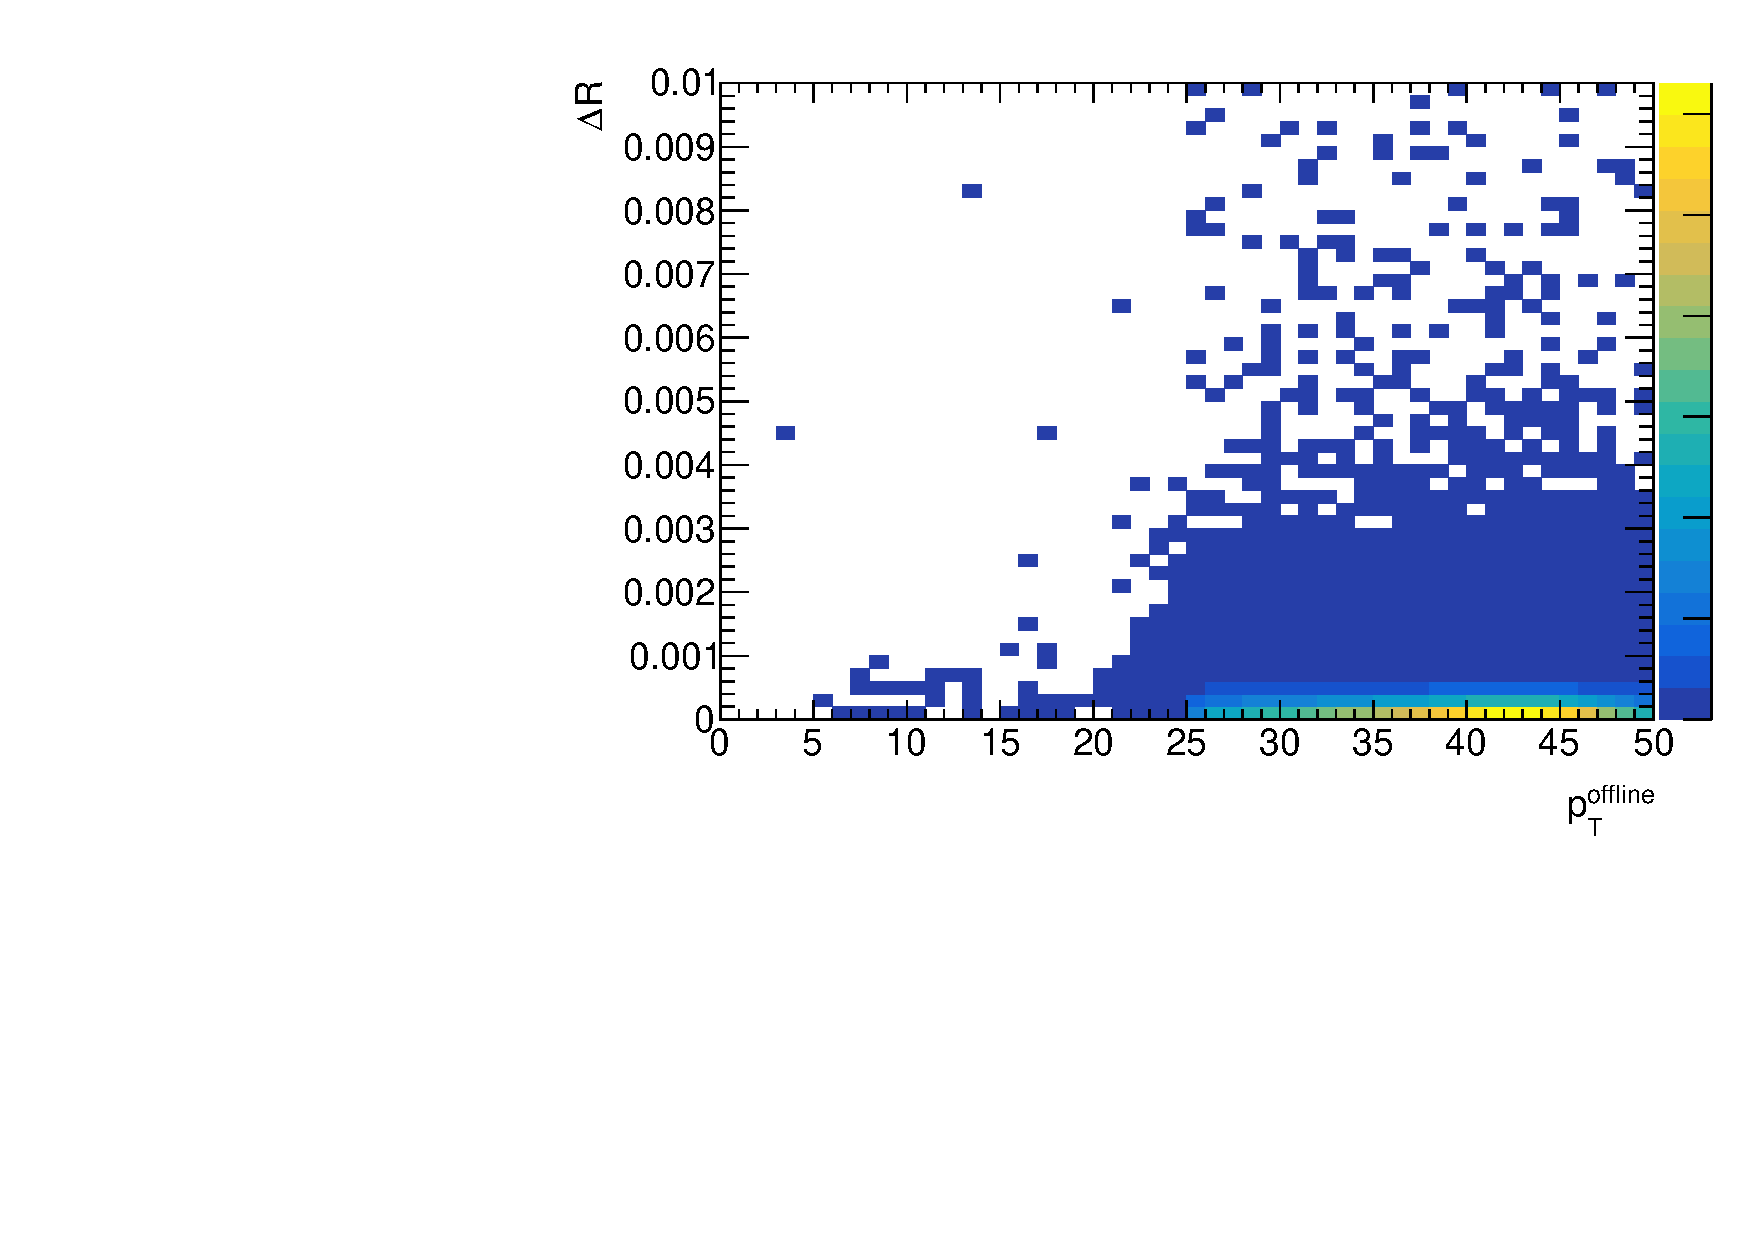
\includegraphics[clip, width=11cm]{fig/3/dR_tag_HLT.pdf}
  \caption{TagミューオンとHLTの$\Delta R$分布。$\Delta R<0.001$ならばTagミューオンがHLTを発行したものとする。}
  \label{fig:tag_HLT}
\end{figure}

次に、Probeミューオンを使用してエンドキャプ部のトリガー性能を評価するために、Probe ミューオンとTGCのヒット情報を一致させる。図~\ref{fig:Probe_TGC}にProbeミューオンとTGCのヒット情報の$\Delta R$を$p_{\rm{T}}$の関数として表した2次元分布を示す。本研究では$\Delta R<0.04$を満たせばProbeミューオンがTGCのヒット情報と一致したものとする。
このProbeミューオンの情報と一致したTGC のヒット情報を使って評価を行う。

\begin{figure}[htb]
  \centering
  %\rule{8cm}{6cm}
  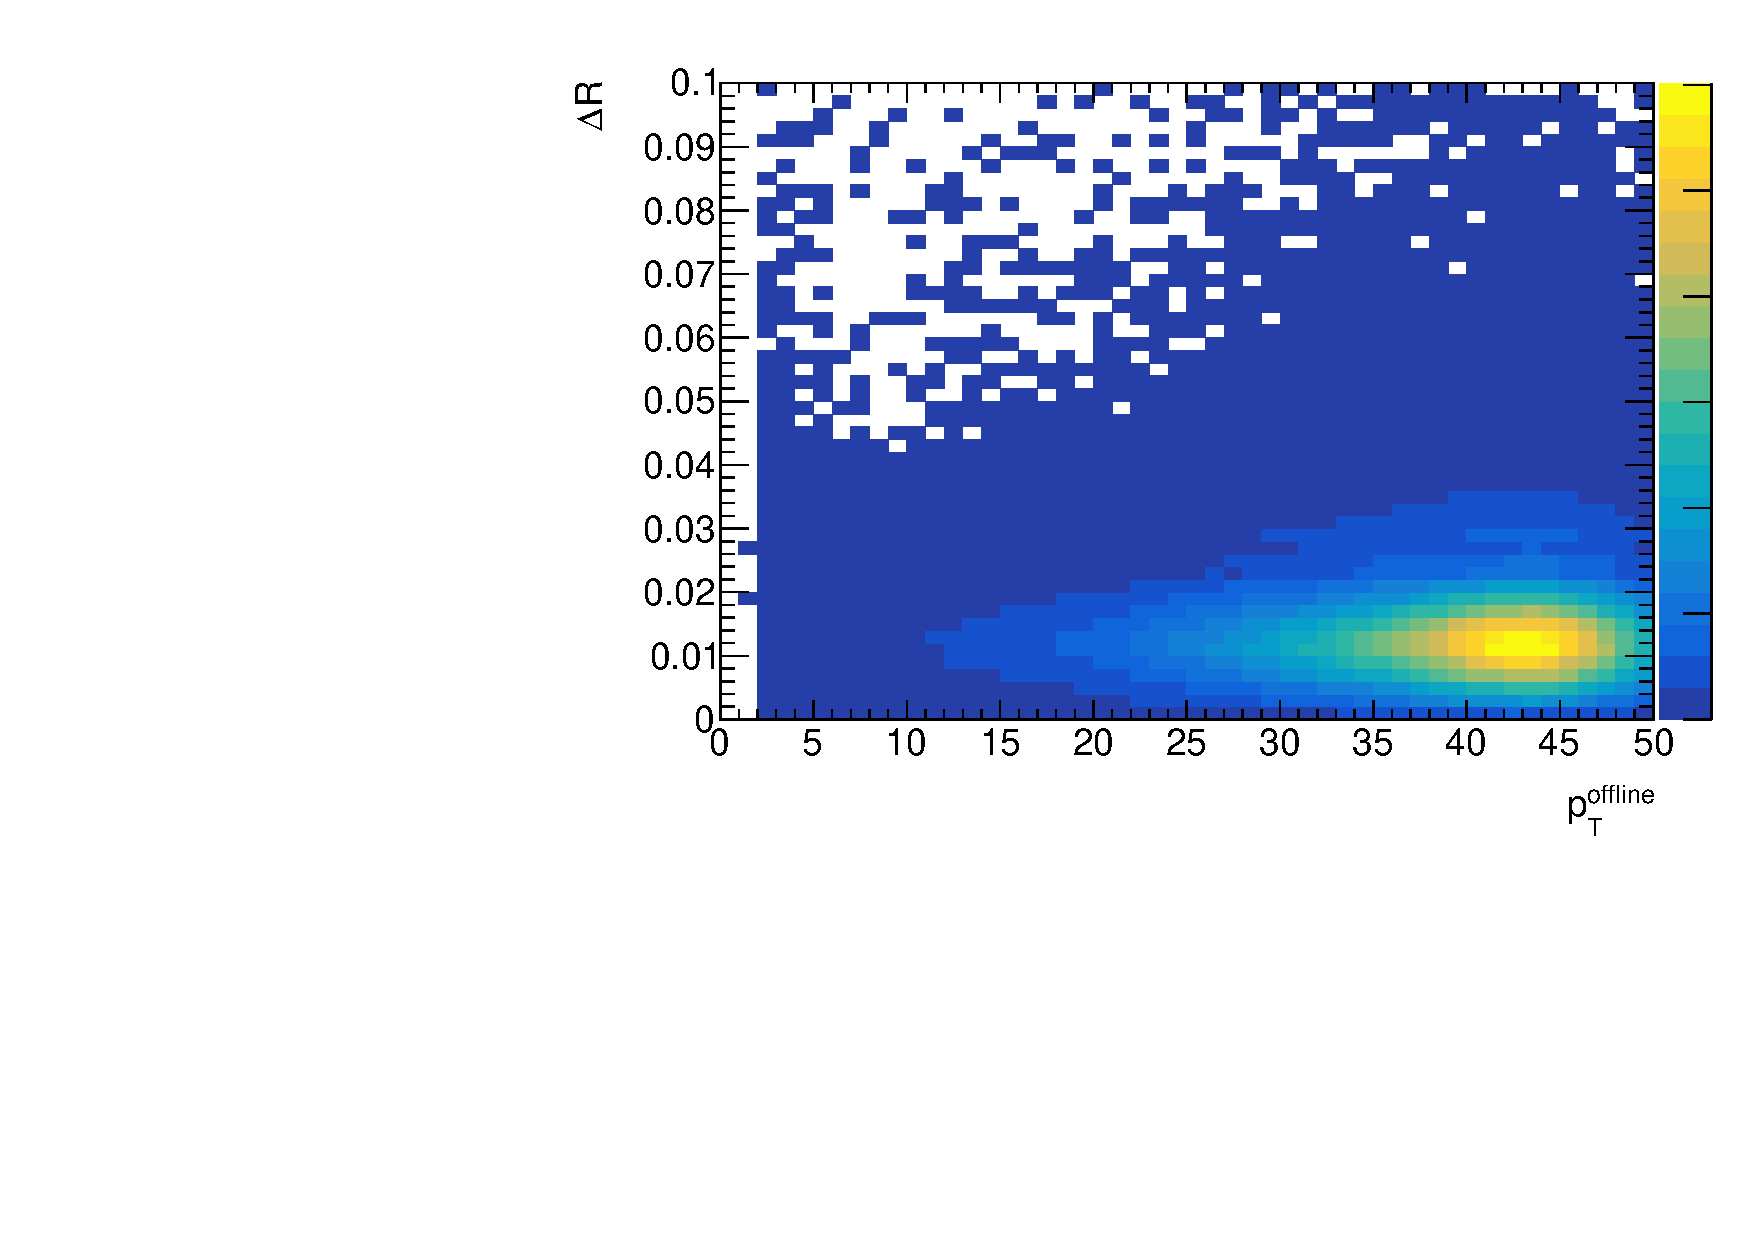
\includegraphics[clip, width=11cm]{fig/3/dR_probe_RoI.pdf}
  \caption{ProbeミューオンとTGCのヒット情報との$\Delta R$分布。$\Delta R< 0.04$ならばProbeミューオンがTGCのヒット情報と一致したものとする。}
  \label{fig:Probe_TGC}
\end{figure}

\subsection{作成したCWの15段階の$p_{\rm{T}}$閾値}
図~\ref{fig:15Eff_CW_Data}に$\mathrm{CW_{Data}}$を用いて15段階の$p_{\rm{T}}$閾値におけるTurn-on curveを示す。評価には2018年Run-2 のデータに対して$Z\rightarrow \mu\mu$によるTag$\&$Probe法を用いた。
$\mathrm{CW_{2022}}$と同様に、本研究の手法で作成した$\mathrm{CW_{Data}}$は15段階に分かれたTurn-on curveを描けていることがわかる。
また、図~\ref{fig:15Eff_CW_Simu}に$\mathrm{CW_{Simu}}$を用いてを要求した15段階の$p_{\rm{T}}$閾値におけるTurn-on curveを示す。評価にはシングルミューオンのシミュレーションサンプルを用いた。
比較のため、図~\ref{fig:Run3_15_MC5} に $\mathrm{CW_{2022}}$を用いた15段階の$p_{\rm{T}}$閾値におけるのTurn-on curveを示す。
こちらも同様に、本研究の手法で作成した$\mathrm{CW_{Simu}}$は15段階に分かれたTurn-on curveを描けていることがわかる。
よって、本研究の手法によって作成された2種類のCWは、2022年度Run-3において使用された$\mathrm{CW_{2022}}$と同様に細かい精度で15段階の判定が可能であることが見て取れる。
ここから、本研究の手法を用いて、15段階の閾値を持ったCWの作成が可能であることが確認できる。
\begin{figure}
    %\centering
    \begin{tabular}{cc}
    \begin{minipage}[b]{0.45\hsize}
        %\centering
        \hspace*{-1cm}
        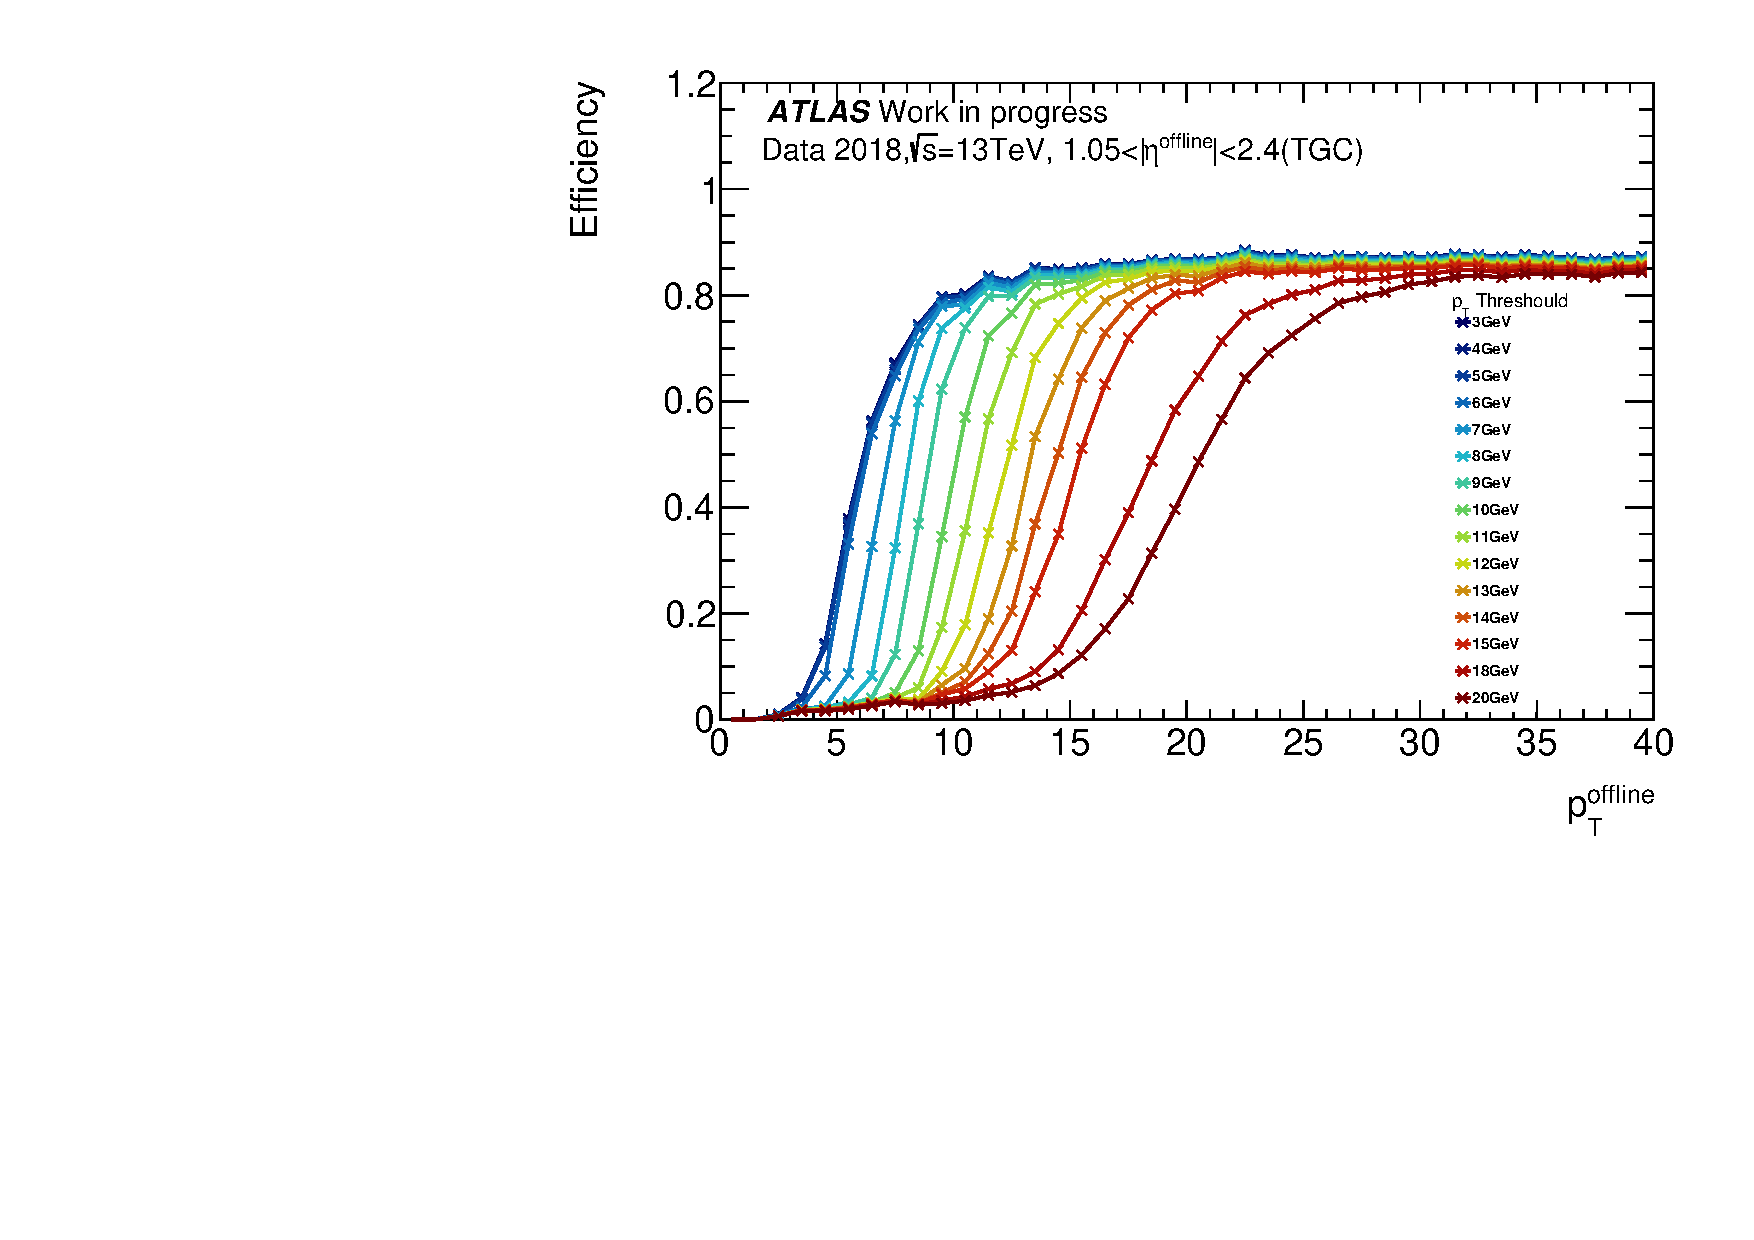
\includegraphics[clip, width=8cm]{fig/5/15_v06_Data.pdf}
        %\vspace{5pt}
        \subcaption{}
        \label{fig:15Eff_CW_Data}
    \end{minipage}&
    %\hfill
    \begin{minipage}[b]{0.45\hsize}
        %\centering
        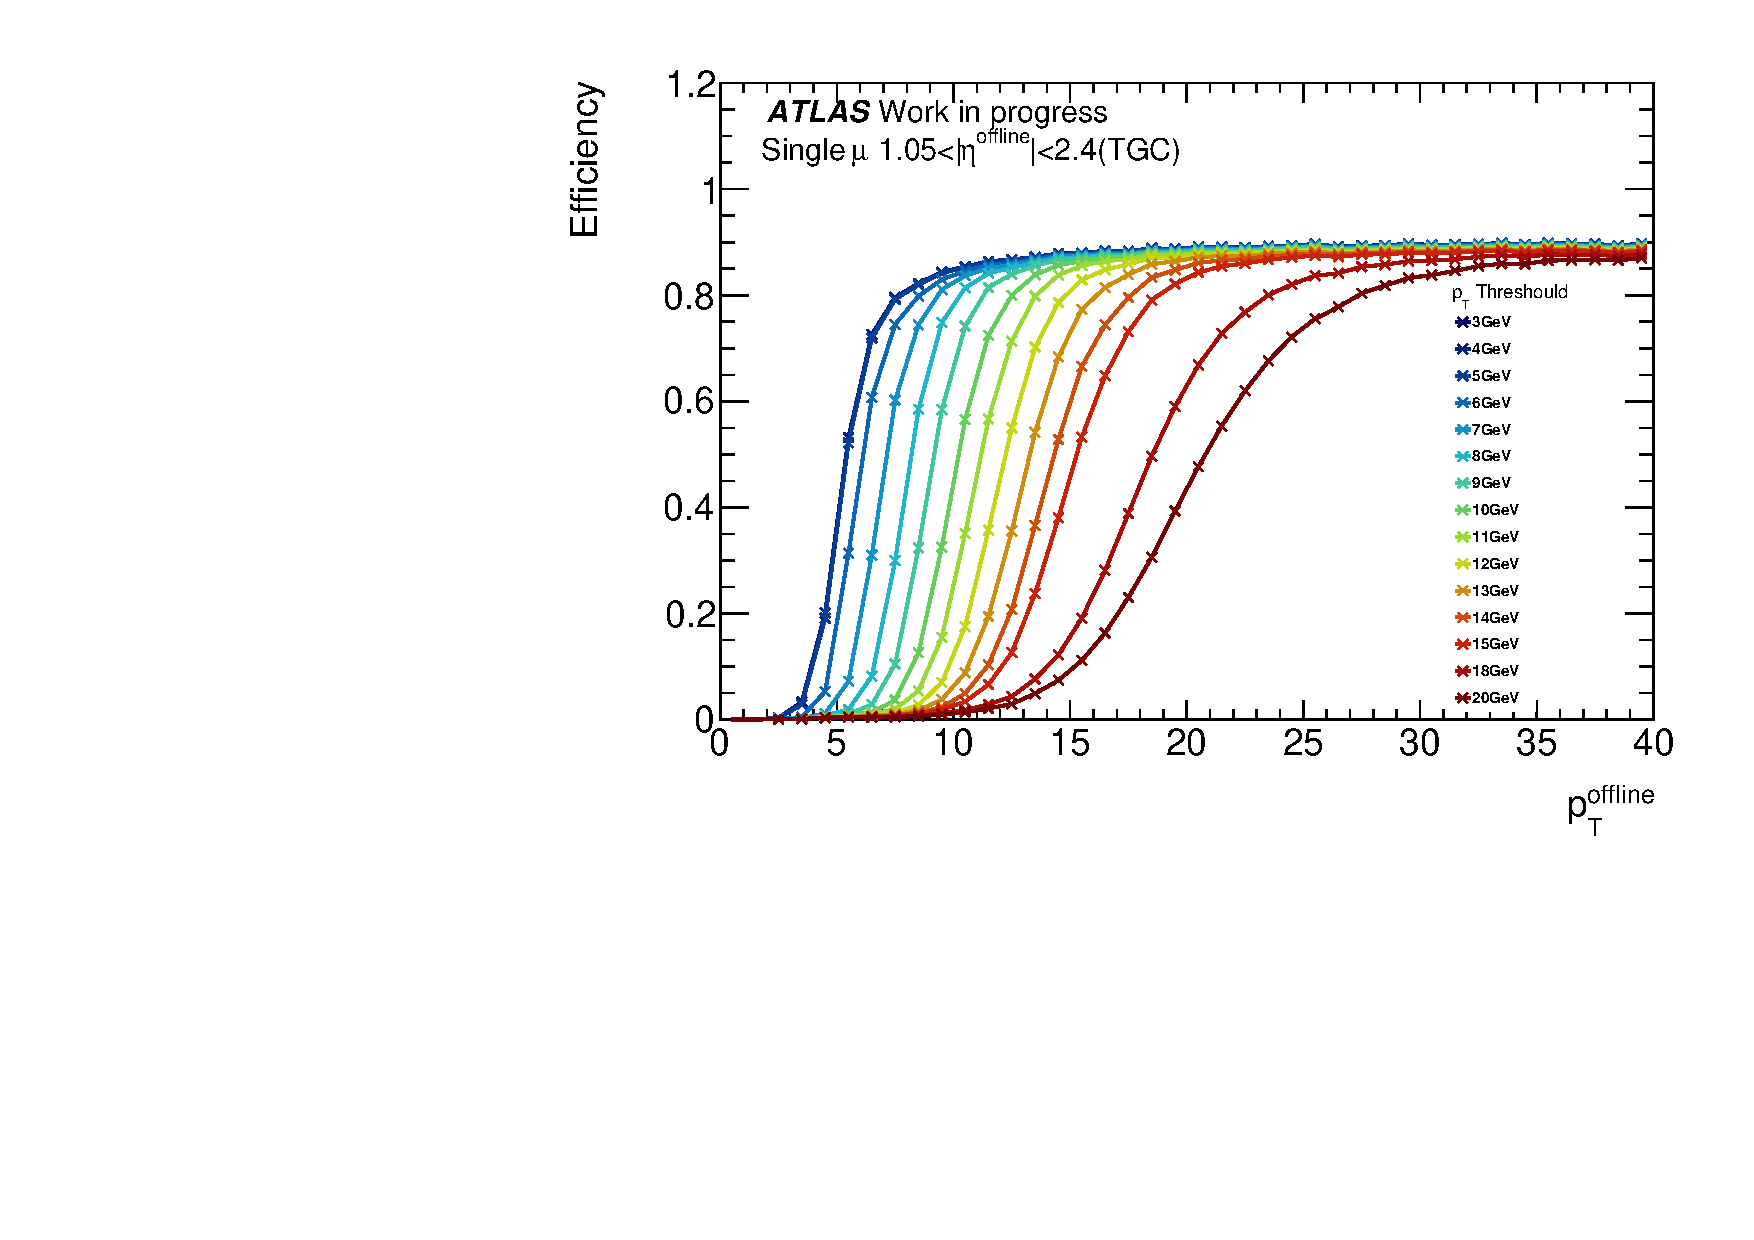
\includegraphics[clip, width=8cm]{fig/5/15_MC_MC.pdf}
        %\vspace{5pt}
        \subcaption{}
        \label{fig:15Eff_CW_Simu}
    \end{minipage}
    \end{tabular}
    \caption{機械学習を用いて作成したCWの15段階の閾値におけるTurn-on curve。(a):実際のデータを用いてトレーニングを行った機械学習から作成したCW。(b): シミュレーションデータを用いてトレーニングを行った機械学習から作成したCW。}
    \label{}
\end{figure}

\begin{figure}[tb]
  \centering
  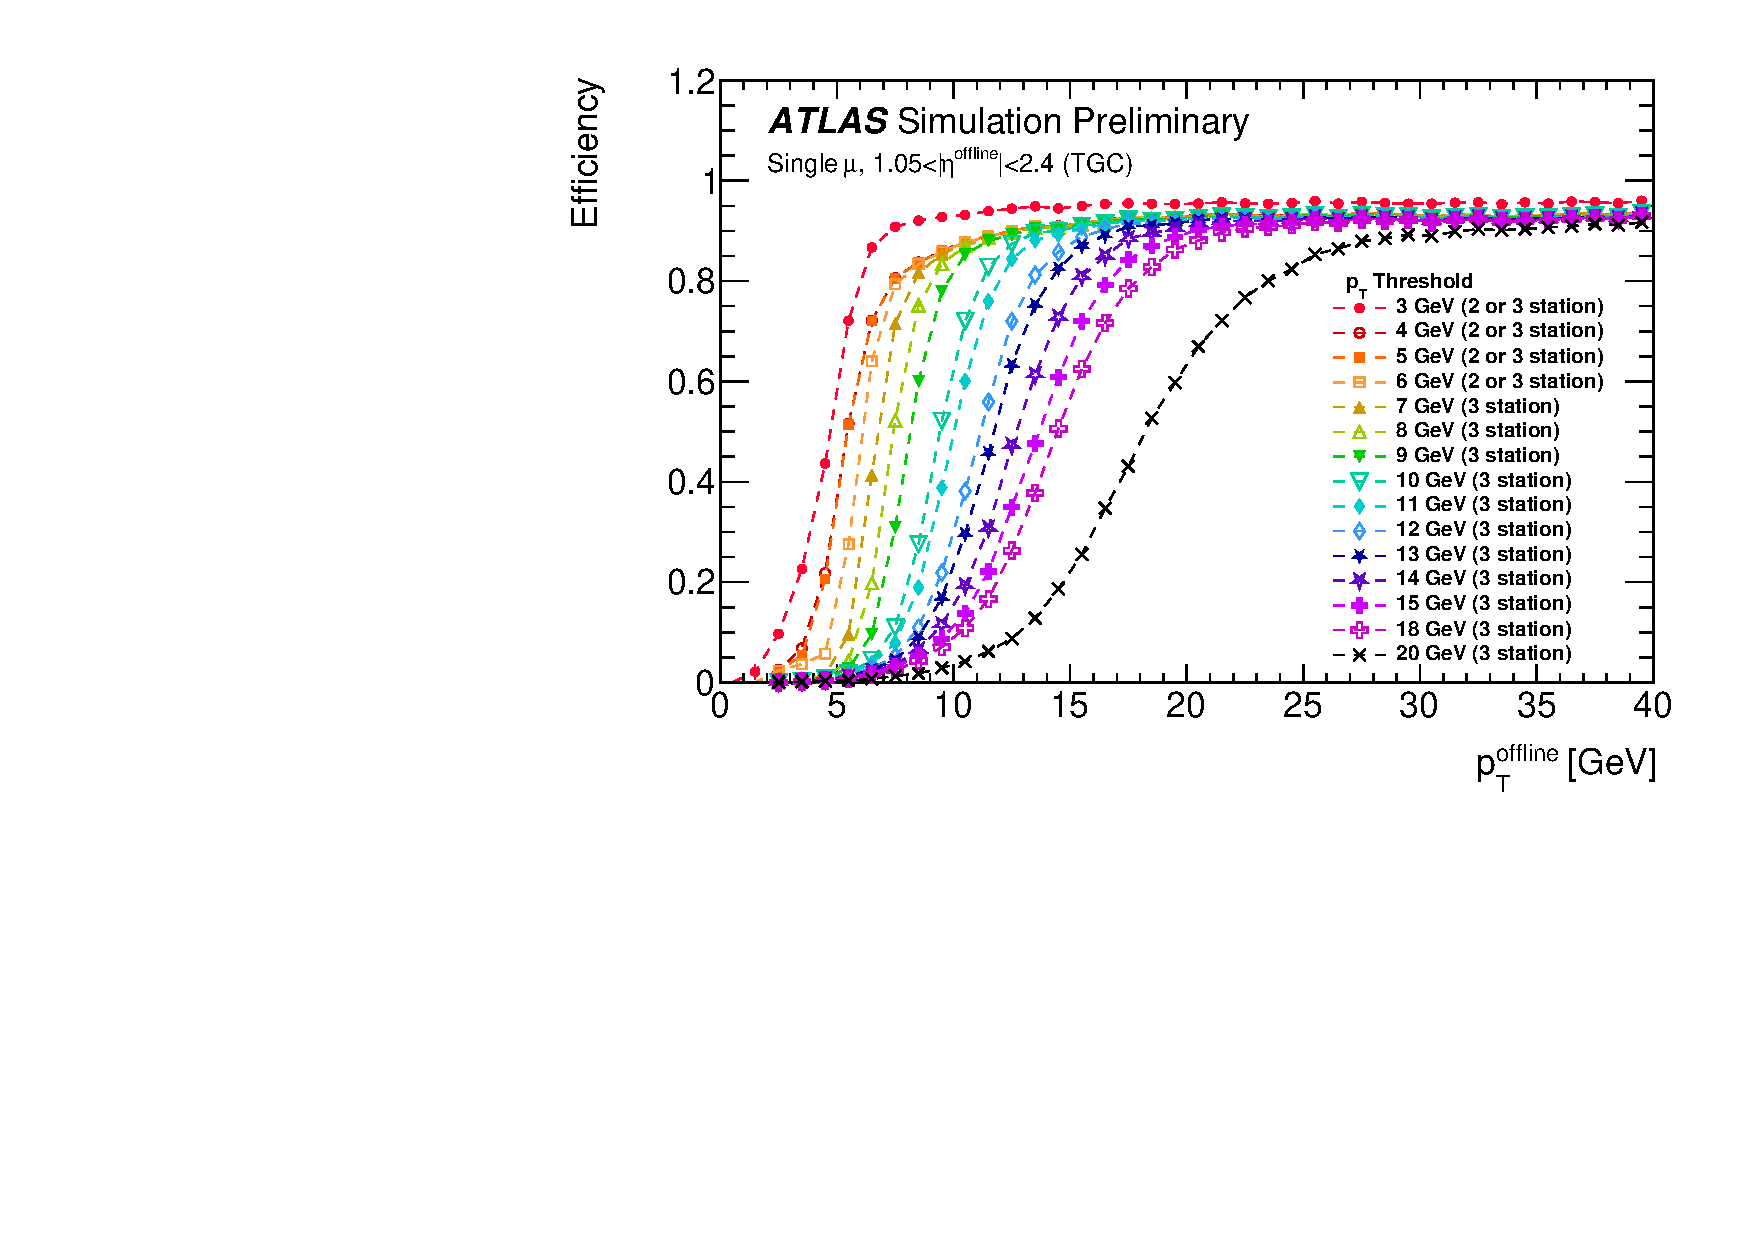
\includegraphics[clip, width=10cm]{fig/3/PLOT-TRIG-2020-01-fig1.pdf}
  \caption{2022年Run-3で使用した15段階閾値のTurn-on curve。シングルミューオンのシミュレーションサンプルに対してのトリガー効率を示している。}
  \label{fig:Run3_15_MC5}
\end{figure}

\subsection{現行のトリガーとのトリガー性能の比較}
次に、それぞれの15段階の$p_{\rm{T}}$閾値のトリガー性能について評価を行う。

\subsubsection{トリガー効率の評価}
まず、$\mathrm{CW_{Simu}}$と$\mathrm{CW_{2022}}$の比較と、$\mathrm{CW_{Data}}$と$\mathrm{CW_{2022}}$の比較を行う。ここでは、トリガー効率$\epsilon$用いてを比較行う。

図~\ref{fig:v05v07}には$p_{\rm{T}}$閾値が14~GeVの時の、$\mathrm{CW_{2022}}$と$\mathrm{CW_{Simu}}$のTurn-on curveの比較を示し、図~\ref{fig:v05v06}には$p_{\rm{T}}$閾値が14~GeVの時の、$\mathrm{CW_{Data}}$を$\mathrm{CW_{2022}}$のTurn-on curveの比較を示す。

2022年度Run-3で使用されている$\mathrm{CW_{2022}}$に比べて、本研究の手法ので作成したCWの方がTurn-on curveの立ち上がりが鋭くなっており、トリガー性能が良くなっていることが見て取れる。
また、図~\ref{fig:v05v07_1_9_Simu}と図~\ref{fig:v05v07_12_20_Simu}、図~\ref{fig:v05v07_1_9_Simu}と図~\ref{fig:v05v07_12_20_Simu}に他の$p_{\rm{T}}$閾値における比較を示す。
15段階の閾値において、本研究の手法によって作成された2種類のCWは、2022年度Run-3において使用された$\mathrm{CW_{2022}}$と同様に鋭く立ち上がっていることが見て取れる。
\begin{figure}
    %\centering
    \begin{tabular}{cc}
    \centering
    \begin{minipage}[b]{0.45\hsize}%
        \centering
        \hspace*{-1.5cm}
        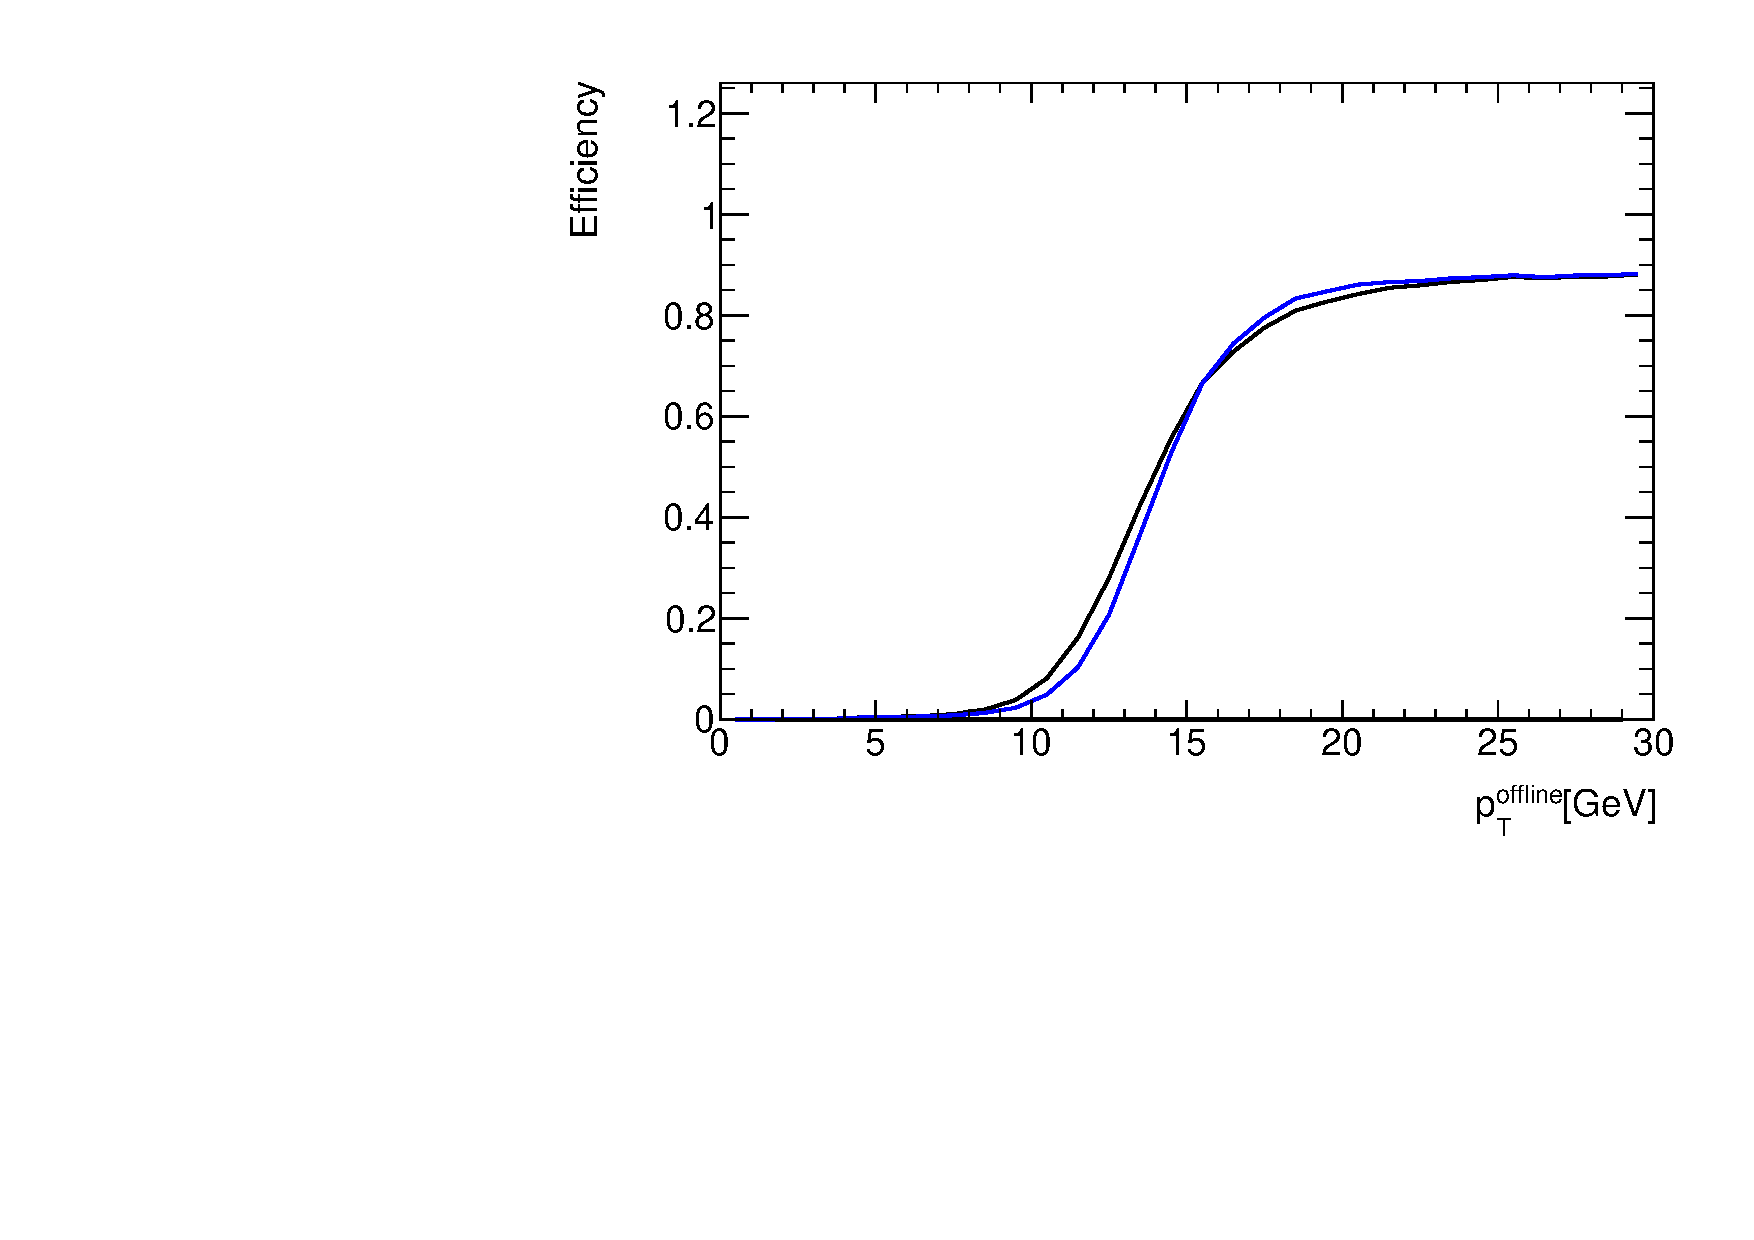
\includegraphics[clip, width=8cm]{fig/5/v05vsv07_MU14.pdf}
        %\vspace{5pt}
        \subcaption{}
        \label{fig:v05v07}
    \end{minipage}%
    %\hfill
    \begin{minipage}[b]{0.7\hsize}%
        \centering
        \hspace*{-0.75cm}
        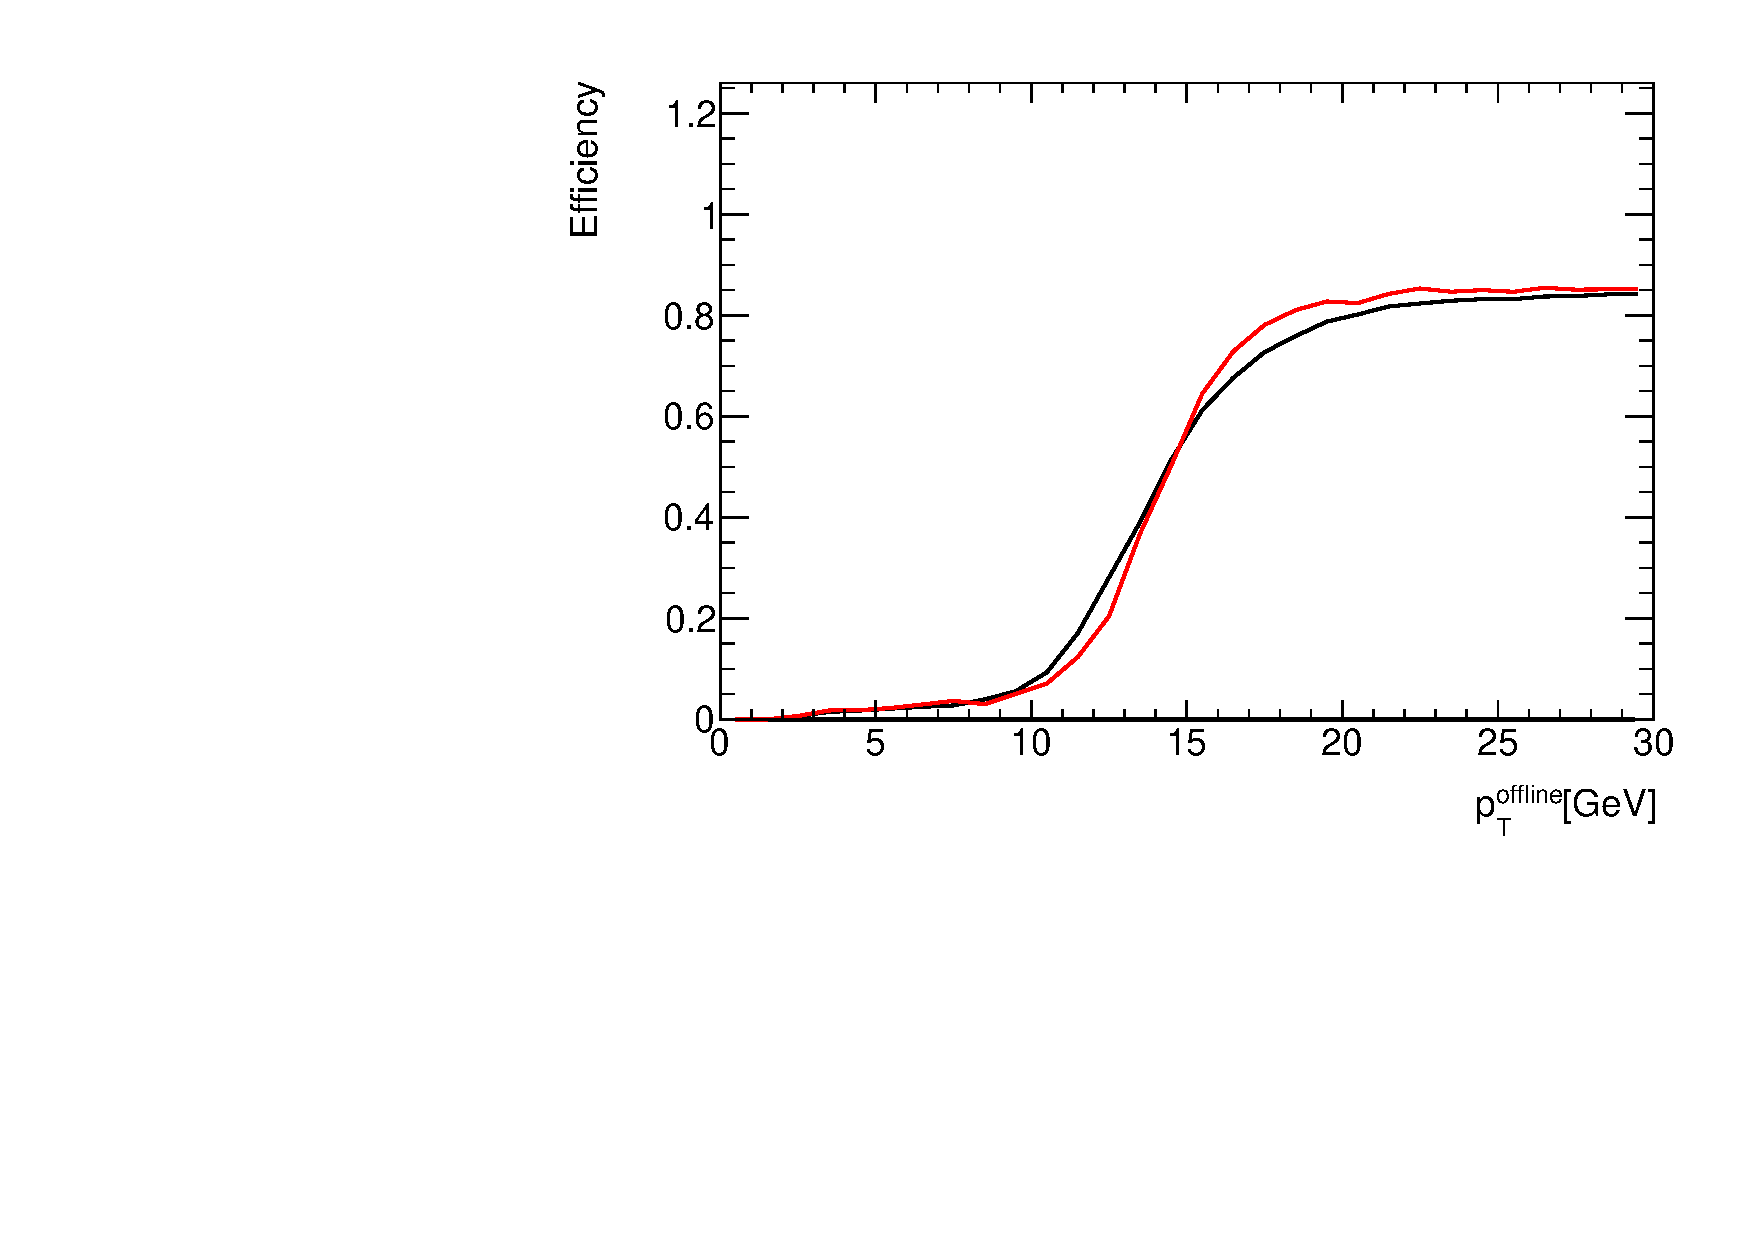
\includegraphics[clip, width=8cm]{fig/5/v05vsv06_MU14.pdf}
        %\vspace{5pt}
        \subcaption{}
        \label{fig:v05v06}
    \end{minipage}%
    \end{tabular}
    \caption{$p_{\rm{T}}$閾値14~GeVにおけるTurn-on curveの比較。(a):$\mathrm{CW_{Simu}}$と$\mathrm{CW_{2022}}$の比較。評価にはシングルミューオンのシミュレーションデータを使用。(b):$\mathrm{CW_{Data}}$と$\mathrm{CW_{2022}}$の比較。評価には2018年Run-2データを使用。}
    \label{fig:v05v07v06}
\end{figure}

\begin{figure}[htb]
  \centering
  %\rule{8cm}{6cm}
  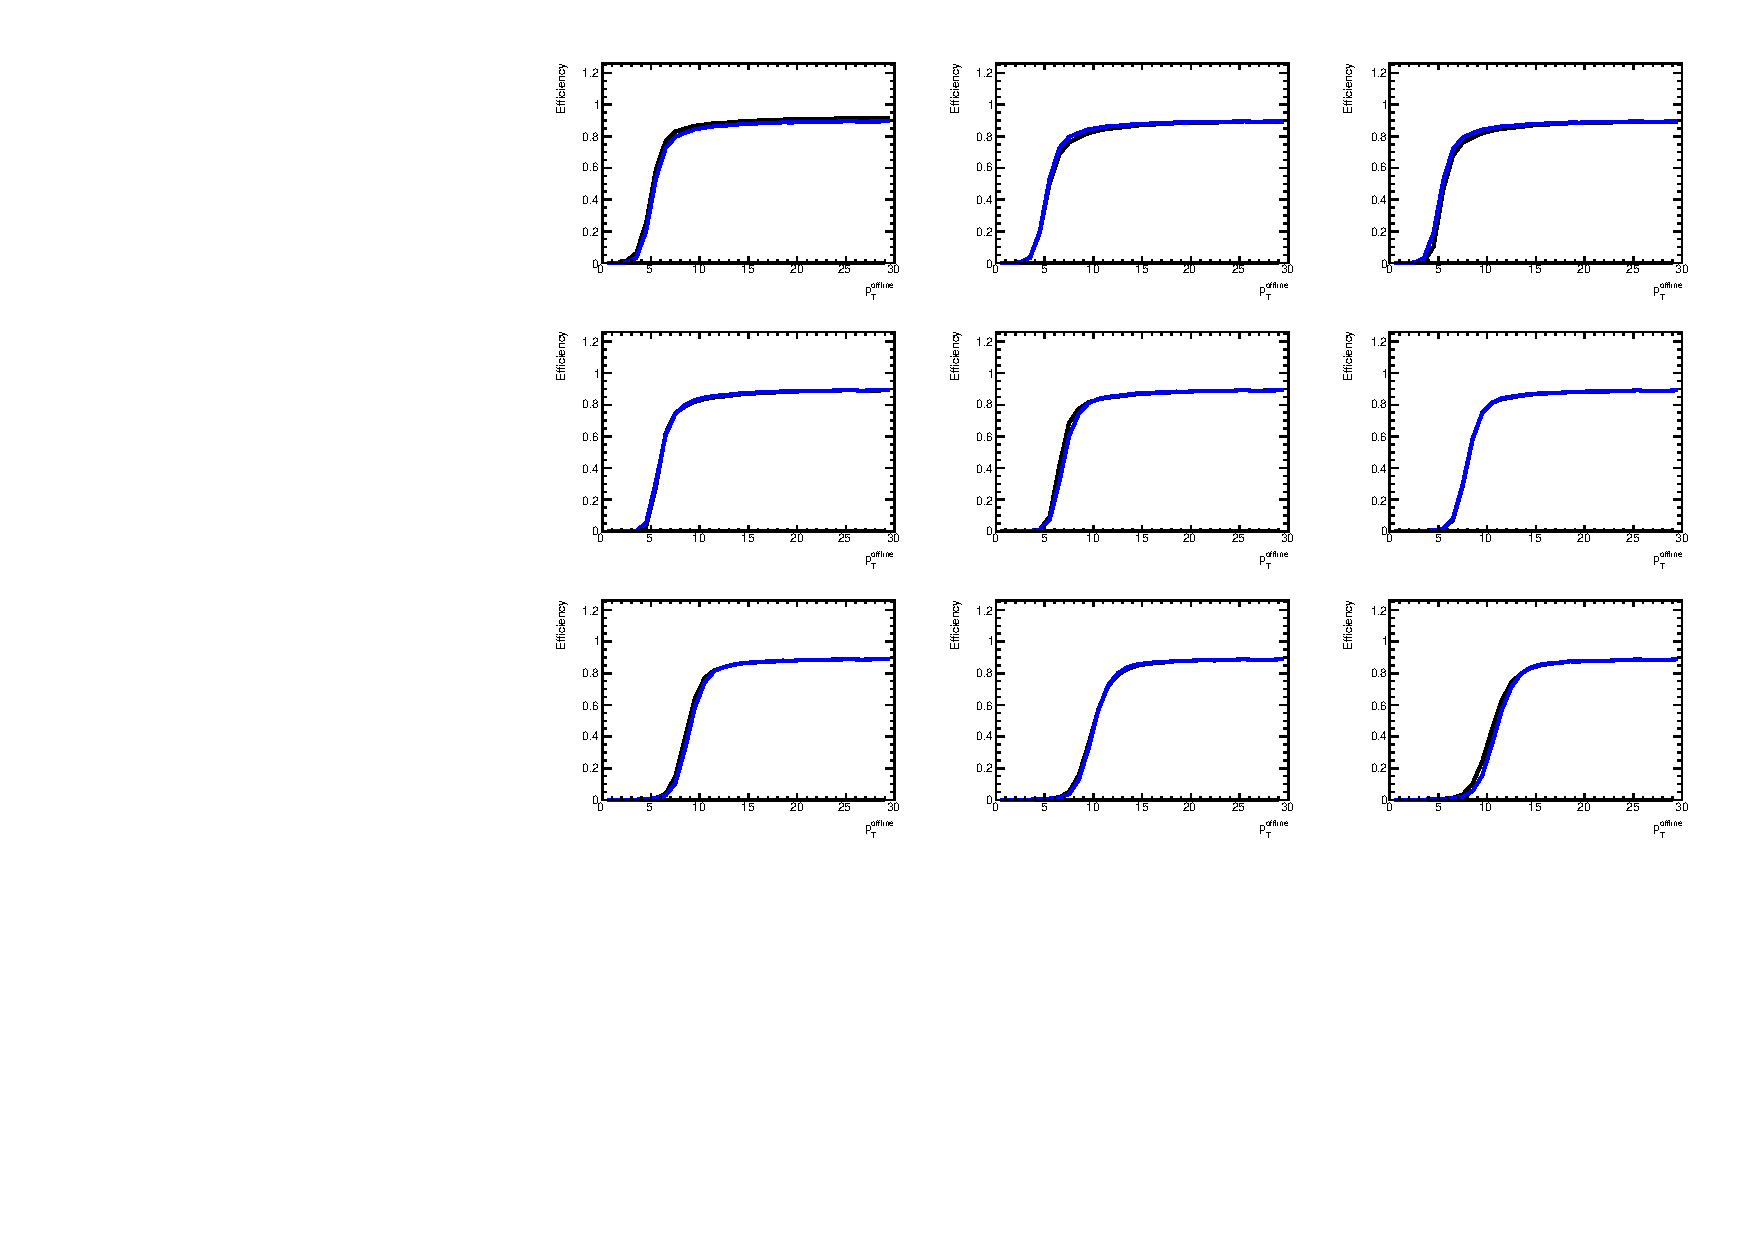
\includegraphics[clip, width=10cm]{fig/5/v05v07_1_9.pdf}
  \caption{$p_{\rm{T}}$閾値3~GeV$\sim$9~GeVにおける$\mathrm{CW_{Simu}}$と$\mathrm{CW_{2022}}$のTurn-on curveの比較。評価にはシングルミューオンのシミュレーションデータを使用した。}
  \label{fig:v05v07_1_9_Simu}
\end{figure}

\begin{figure}[htb]
  \centering
  %\rule{8cm}{6cm}
  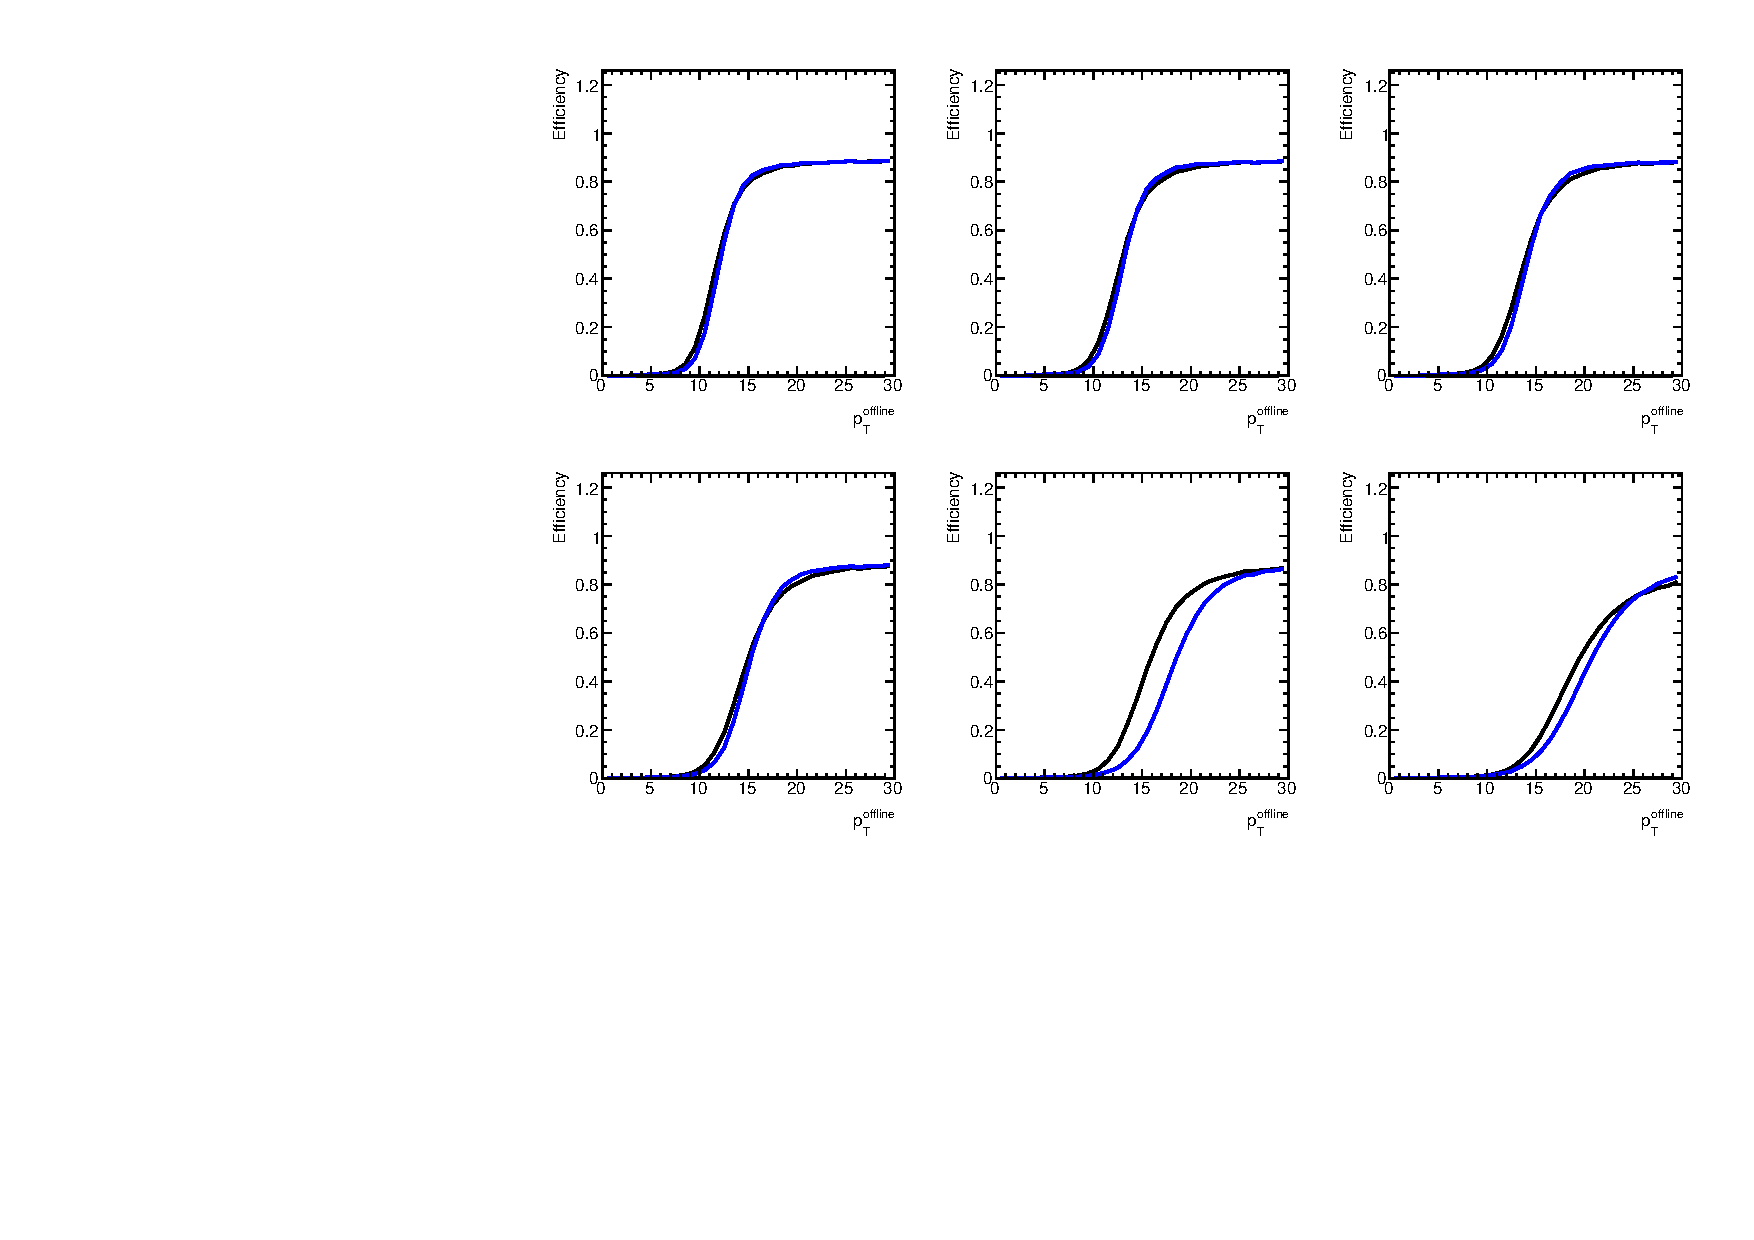
\includegraphics[clip, width=10cm]{fig/5/v05v07_10_15.pdf}
  \caption{$p_{\rm{T}}$閾値10~GeV$\sim$20~GeVにおける$\mathrm{CW_{Simu}}$と$\mathrm{CW_{2022}}$のTurn-on curveの比較。評価にはシングルミューオンのシミュレーションデータを使用した。}
  \label{fig:v05v07_12_20_Simu}
\end{figure}

\begin{figure}[htb]
  \centering
  %\rule{8cm}{6cm}
  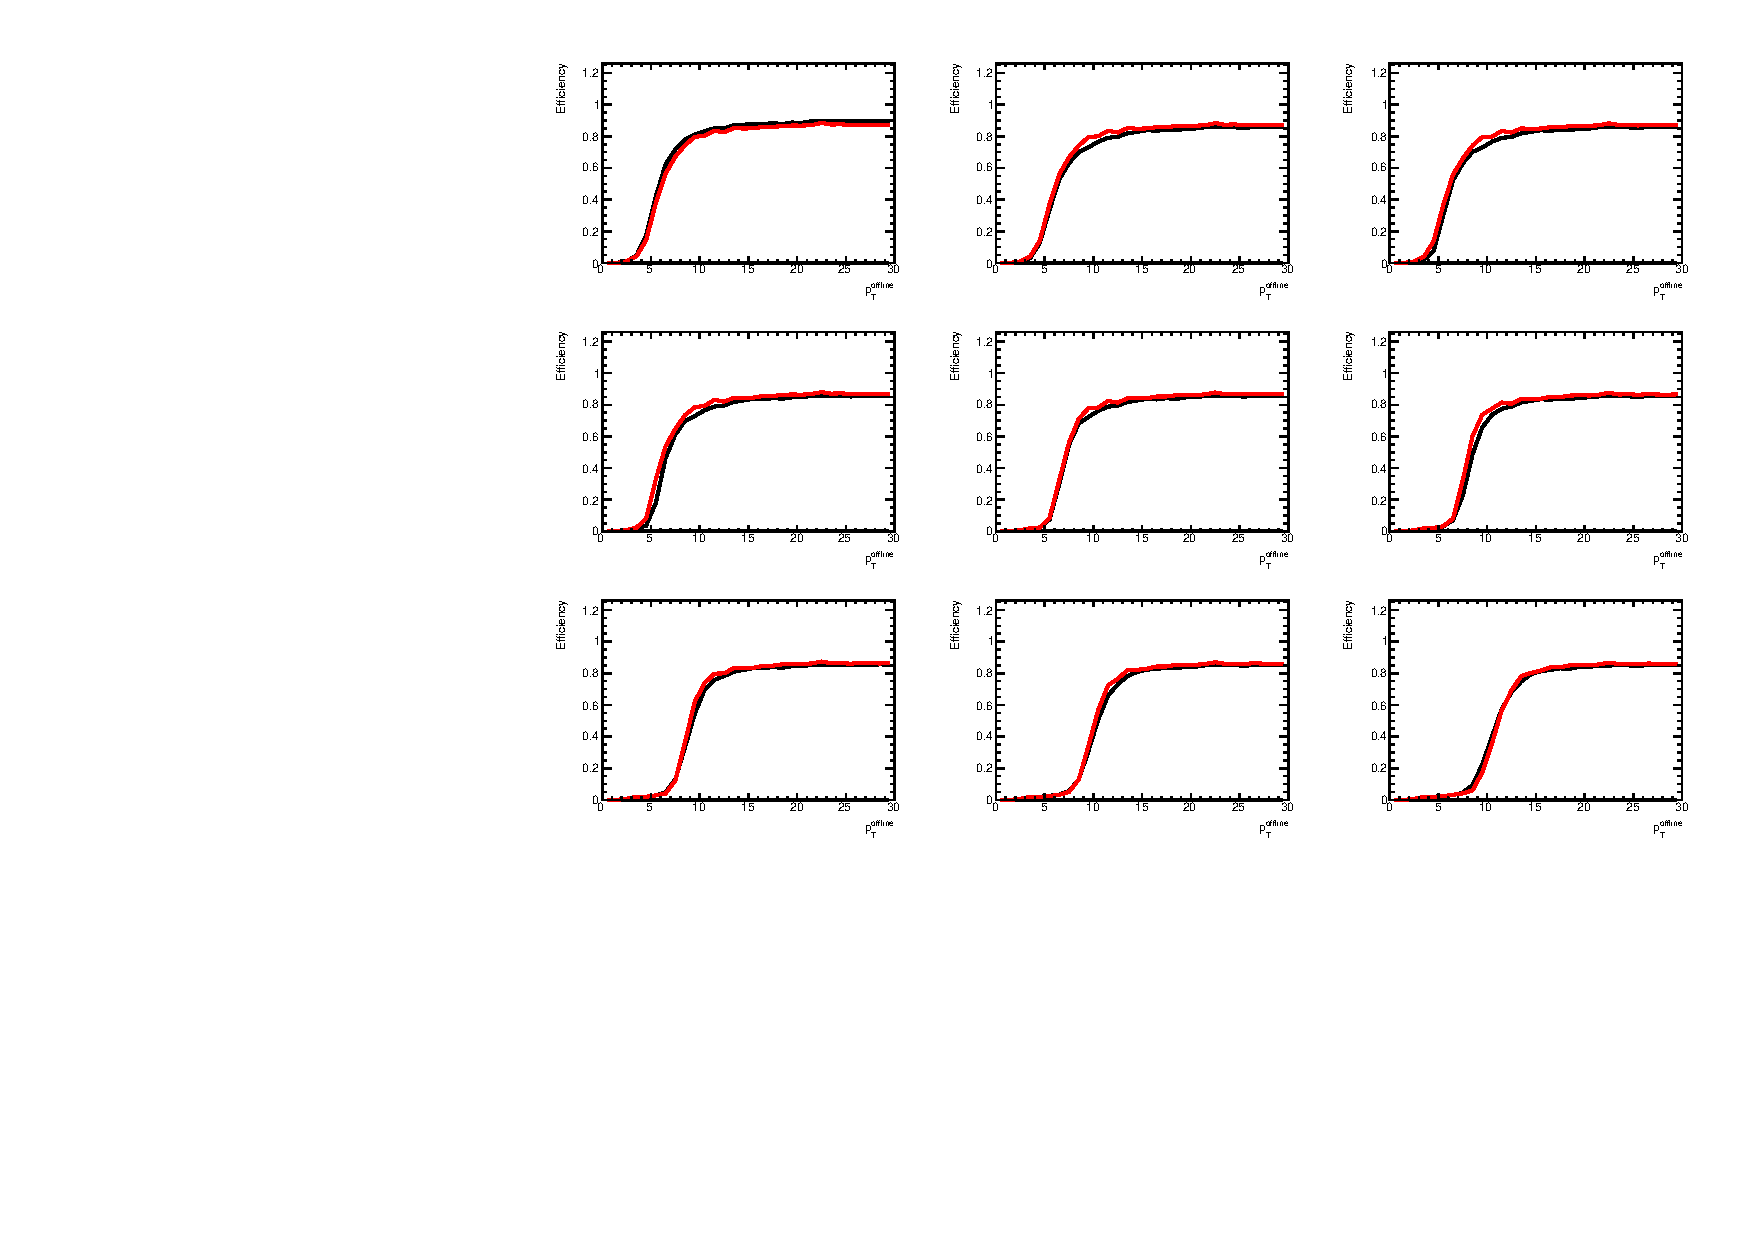
\includegraphics[clip, width=10cm]{fig/5/v05v06_1_9.pdf}
  \caption{$p_{\rm{T}}$閾値3~GeV$\sim$ 9~GeVにおける$\mathrm{CW_{Data}}$と$\mathrm{CW_{2022}}$のTurn-on curveの比較。評価には2018年Run-3のデータを使用した。}
  \label{fig:v05v06_1_9_Data}
\end{figure}

\begin{figure}[htb]
  \centering
  %\rule{8cm}{6cm}
  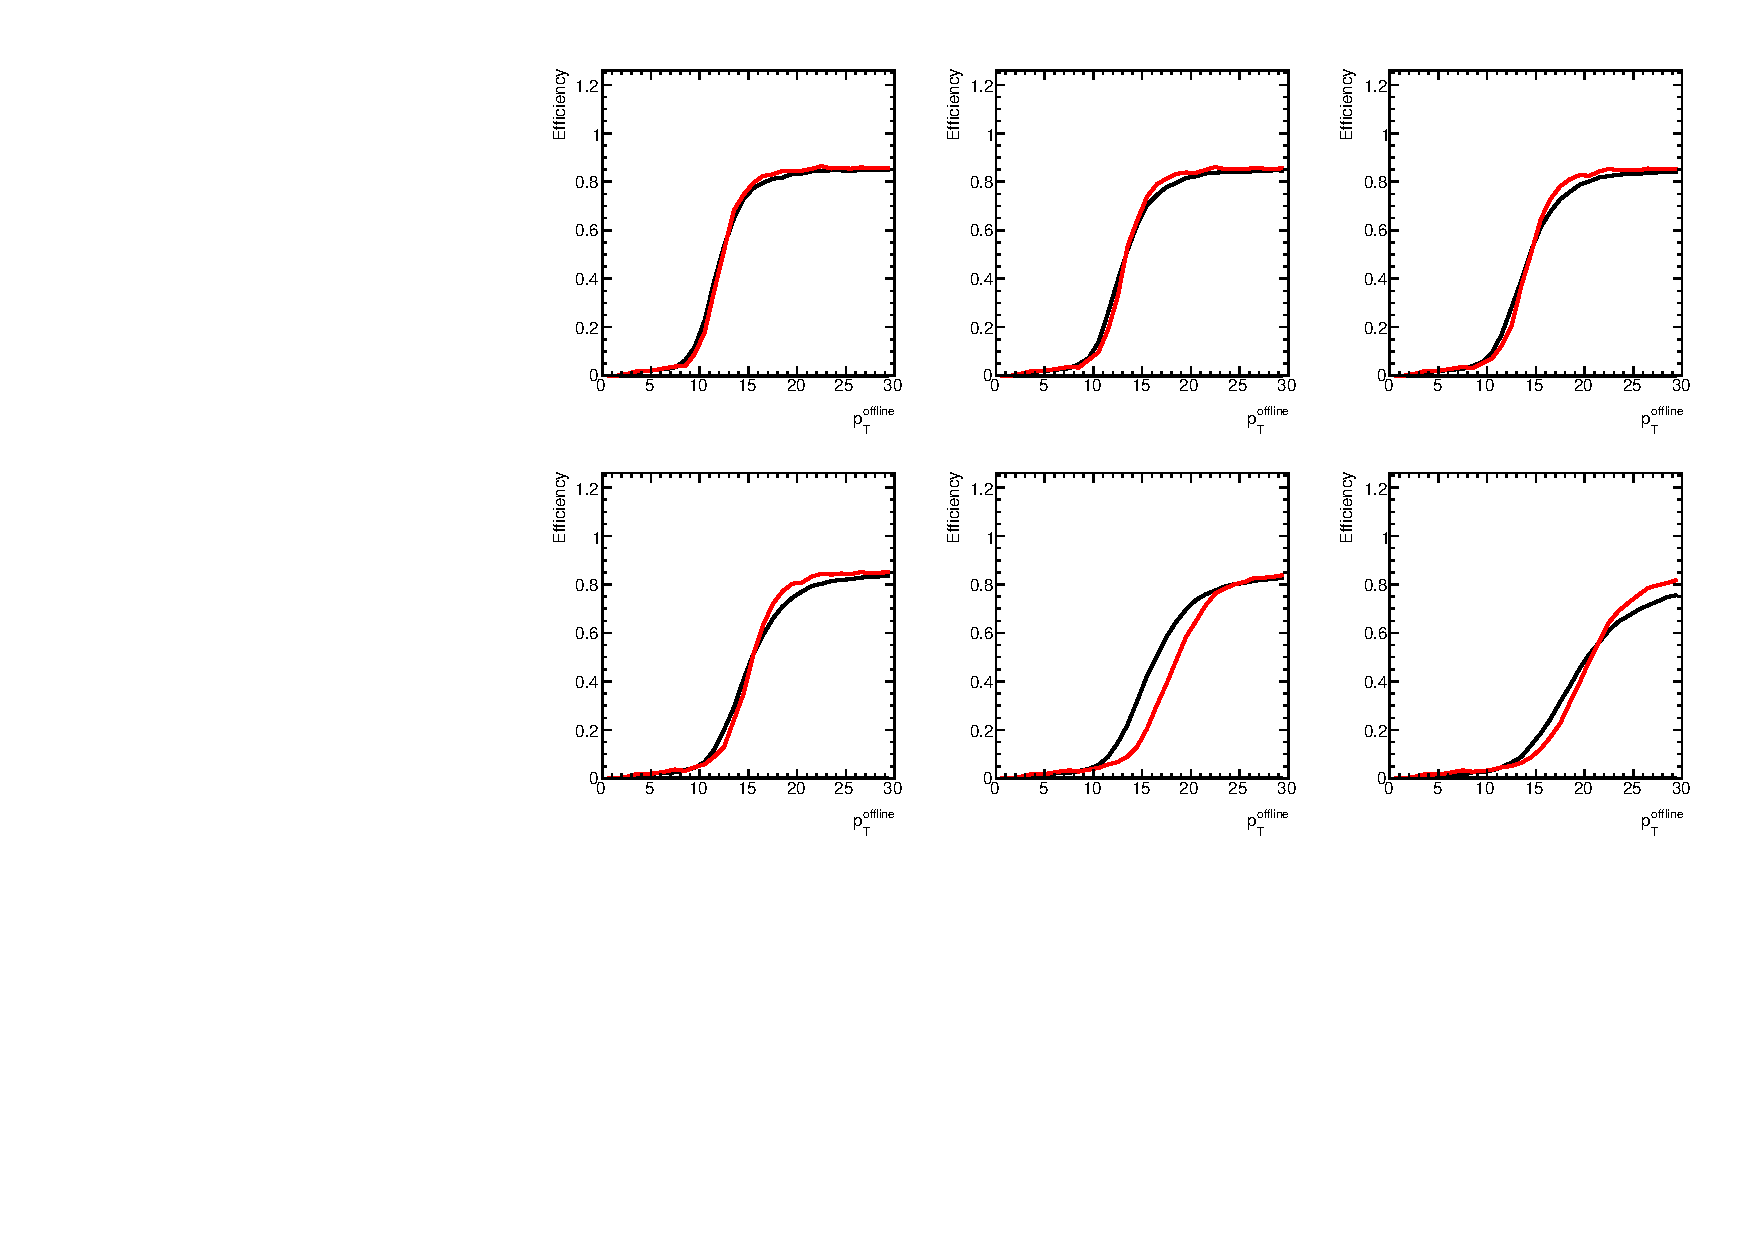
\includegraphics[clip, width=10cm]{fig/5/v05v06_10_15.pdf}
  \caption{$p_{\rm{T}}$閾値10~GeV$\sim$ 20~GeVにおける$\mathrm{CW_{Data}}$と$\mathrm{CW_{2022}}$のTurn-on curveの比較。評価には2018年Run-3のデータを使用した。}
  \label{fig:v05v06_10_15_Data}
\end{figure}

さらに、これらのTurn-on curveに式~\eqref{equ:fitting}によるフィッティングを行い、パラメータの比較を行う。
図~\ref{fig:Resolution_v07v05}に$\mathrm{CW_{Simu}}$と$\mathrm{CW_{2022}}$のEffective thresholdに対するResolitionの比較、図~\ref{fig:Resolution_v06v05}に$\mathrm{CW_{Data}}$と$\mathrm{CW_{2022}}$のEffective thresholdに対するResolitionの比較を示す。
また、図~\ref{fig:Plateau_v07v05}に$\mathrm{CW_{Simu}}$と$\mathrm{CW_{2022}}$のEffective thresholdに対するPlateau Efficiencyの比較、図~\ref{fig:Plateau_v06v05}に$\mathrm{CW_{Data}}$と$\mathrm{CW_{2022}}$のEffective thresholdに対するPlateau Efficiencyの比較を示す。
2018年Run-3で使用された$\mathrm{CW_{2022}}$と比べて、本研究の手法で作成したCWは全体的にPlateau Efficiencyが向上している。
また、本研究で作成したCWは全体的にResolutionの値が小さくなっており、Resolutionの改善がみられる。しかし、低いEffective thresholdのトリガーにおいては、Resolutionの悪化が見られた一方でPlateau Efficiencyは向上していることから、低い$p_{\rm{T}}$閾値の領域が増えたことにより、その領域に入るミューオンの数は増えたが、その分間違った判定をすることが多くなったことを表している。
\begin{figure}
    %\centering
    \begin{tabular}{cc}
    \centering
    \begin{minipage}[b]{0.45\hsize}%
        \centering
        \hspace*{-1.5cm}
        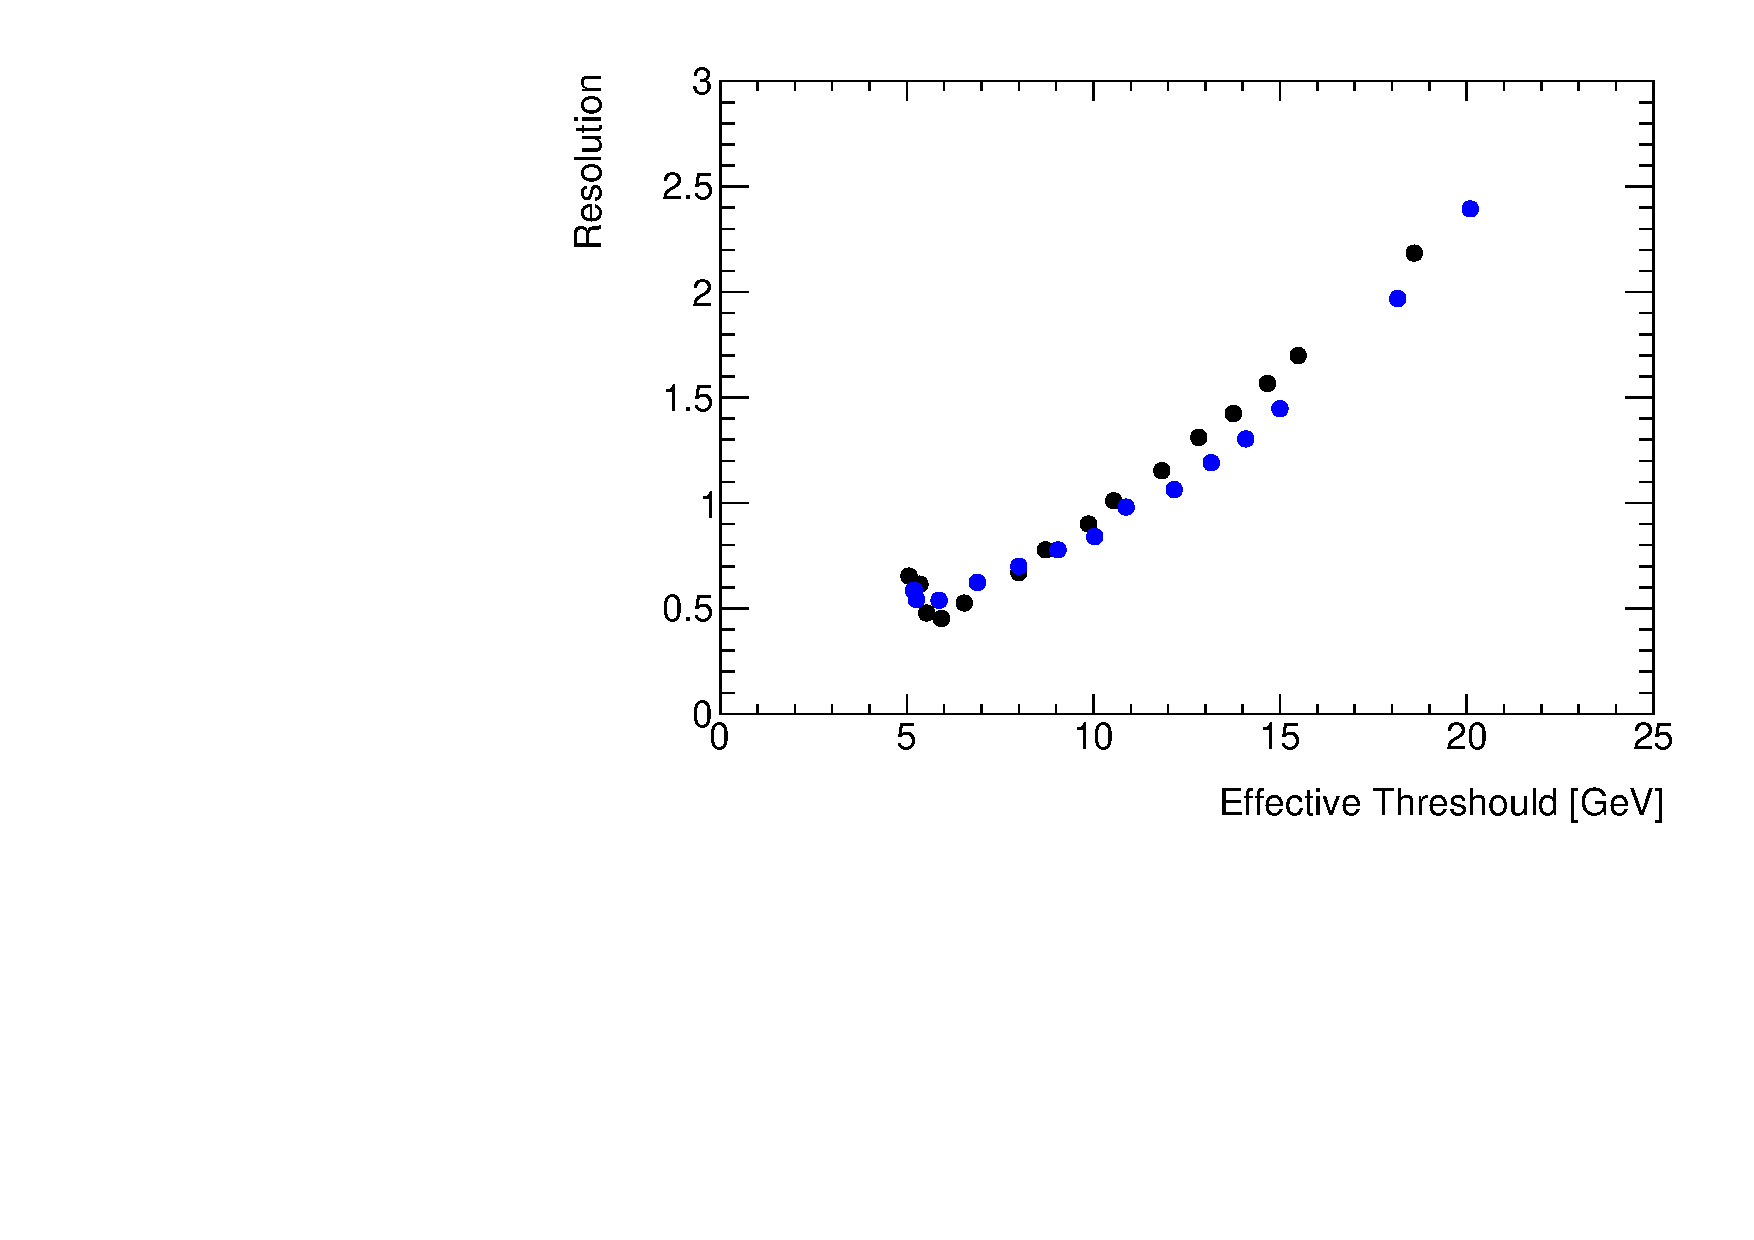
\includegraphics[clip, width=8cm]{fig/4/v05vsv07_Resolution.pdf}
        %\vspace{5pt}
        \subcaption{}
        \label{fig:Resolution_v07v05}
    \end{minipage}%
    %\hfill
    \begin{minipage}[b]{0.7\hsize}%
        \centering
        \hspace*{-0.75cm}
        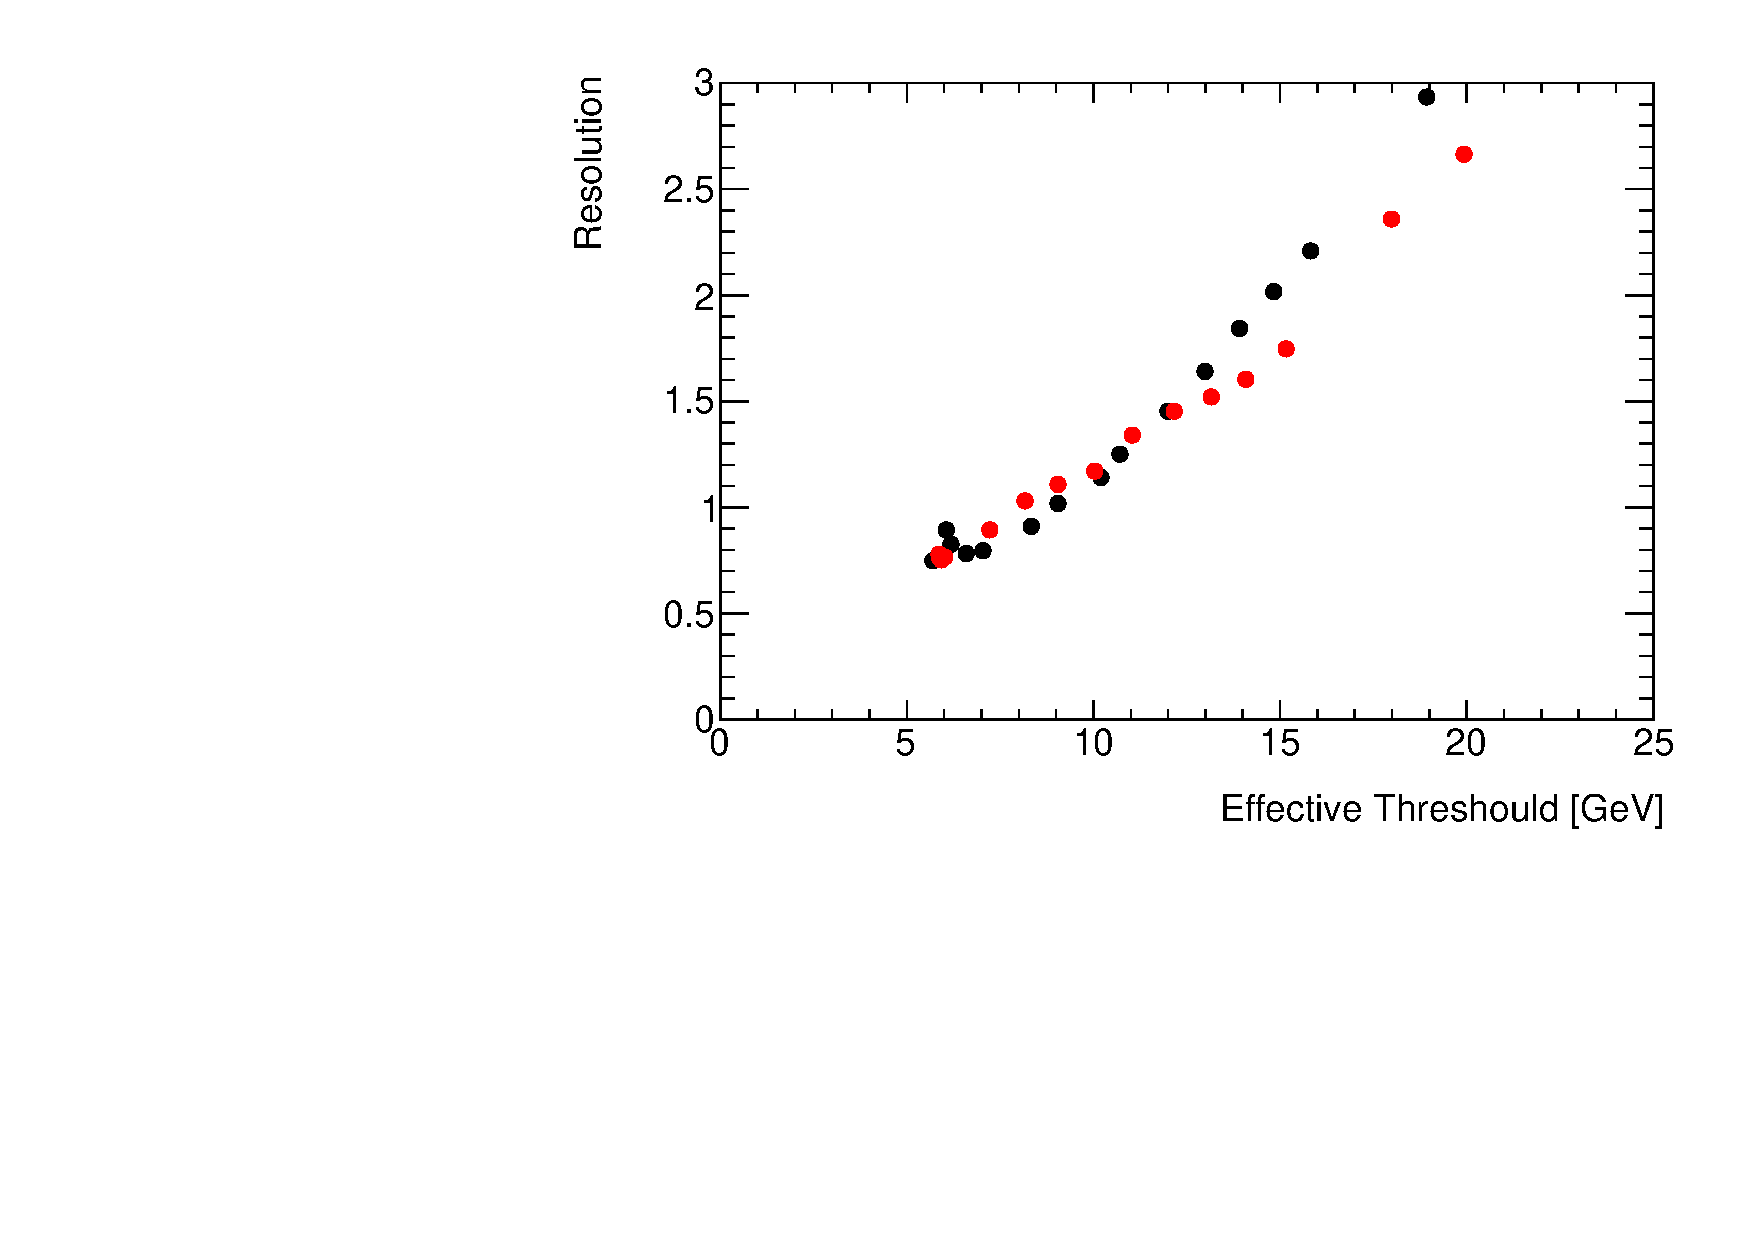
\includegraphics[clip, width=8cm]{fig/4/v05vsv06_Resolution.pdf}
        %\vspace{5pt}
        \subcaption{}
        \label{fig:Resolution_v05v06}
    \end{minipage}%
    \end{tabular}
    \caption{各$p_{\rm{T}}$閾値におけるTurn-on curveのEffective thresholdにおけるResolutionの比較。(a):$\mathrm{CW_{Simu}}$と$\mathrm{CW_{2022}}$の比較。(b):$\mathrm{CW_{Data}}$と$\mathrm{CW_{2022}}$の比較。}
    \label{fig:Resolution_v07v06v05}
\end{figure}

\begin{figure}
    %\centering
    \begin{tabular}{cc}
    \centering
    \begin{minipage}[b]{0.45\hsize}%
        \centering
        \hspace*{-1.5cm}
        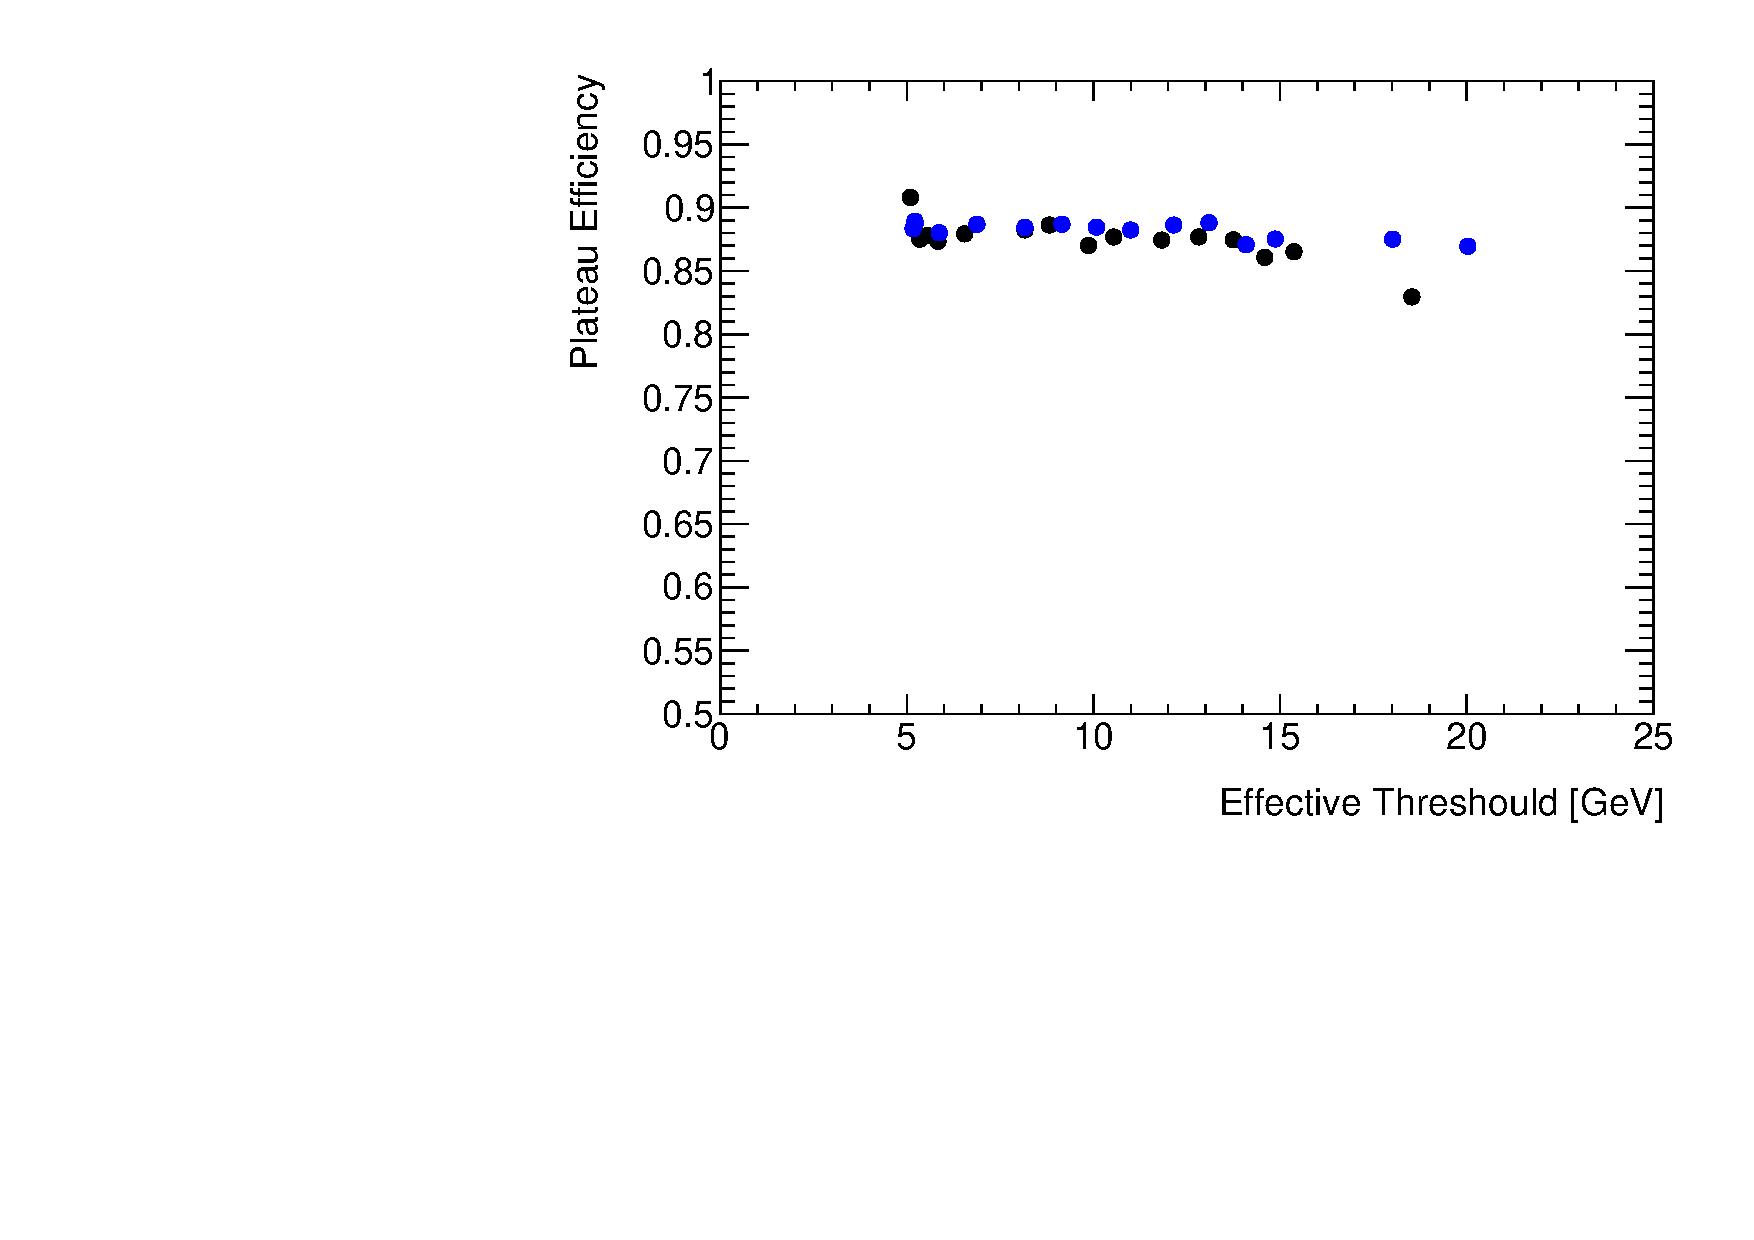
\includegraphics[clip, width=8cm]{fig/4/v05vsv07_Plateau.pdf}
        %\vspace{5pt}
        \subcaption{}
        \label{fig:Plateau_v07v05}
    \end{minipage}%
    %\hfill
    \begin{minipage}[b]{0.7\hsize}%
        \centering
        \hspace*{-0.75cm}
        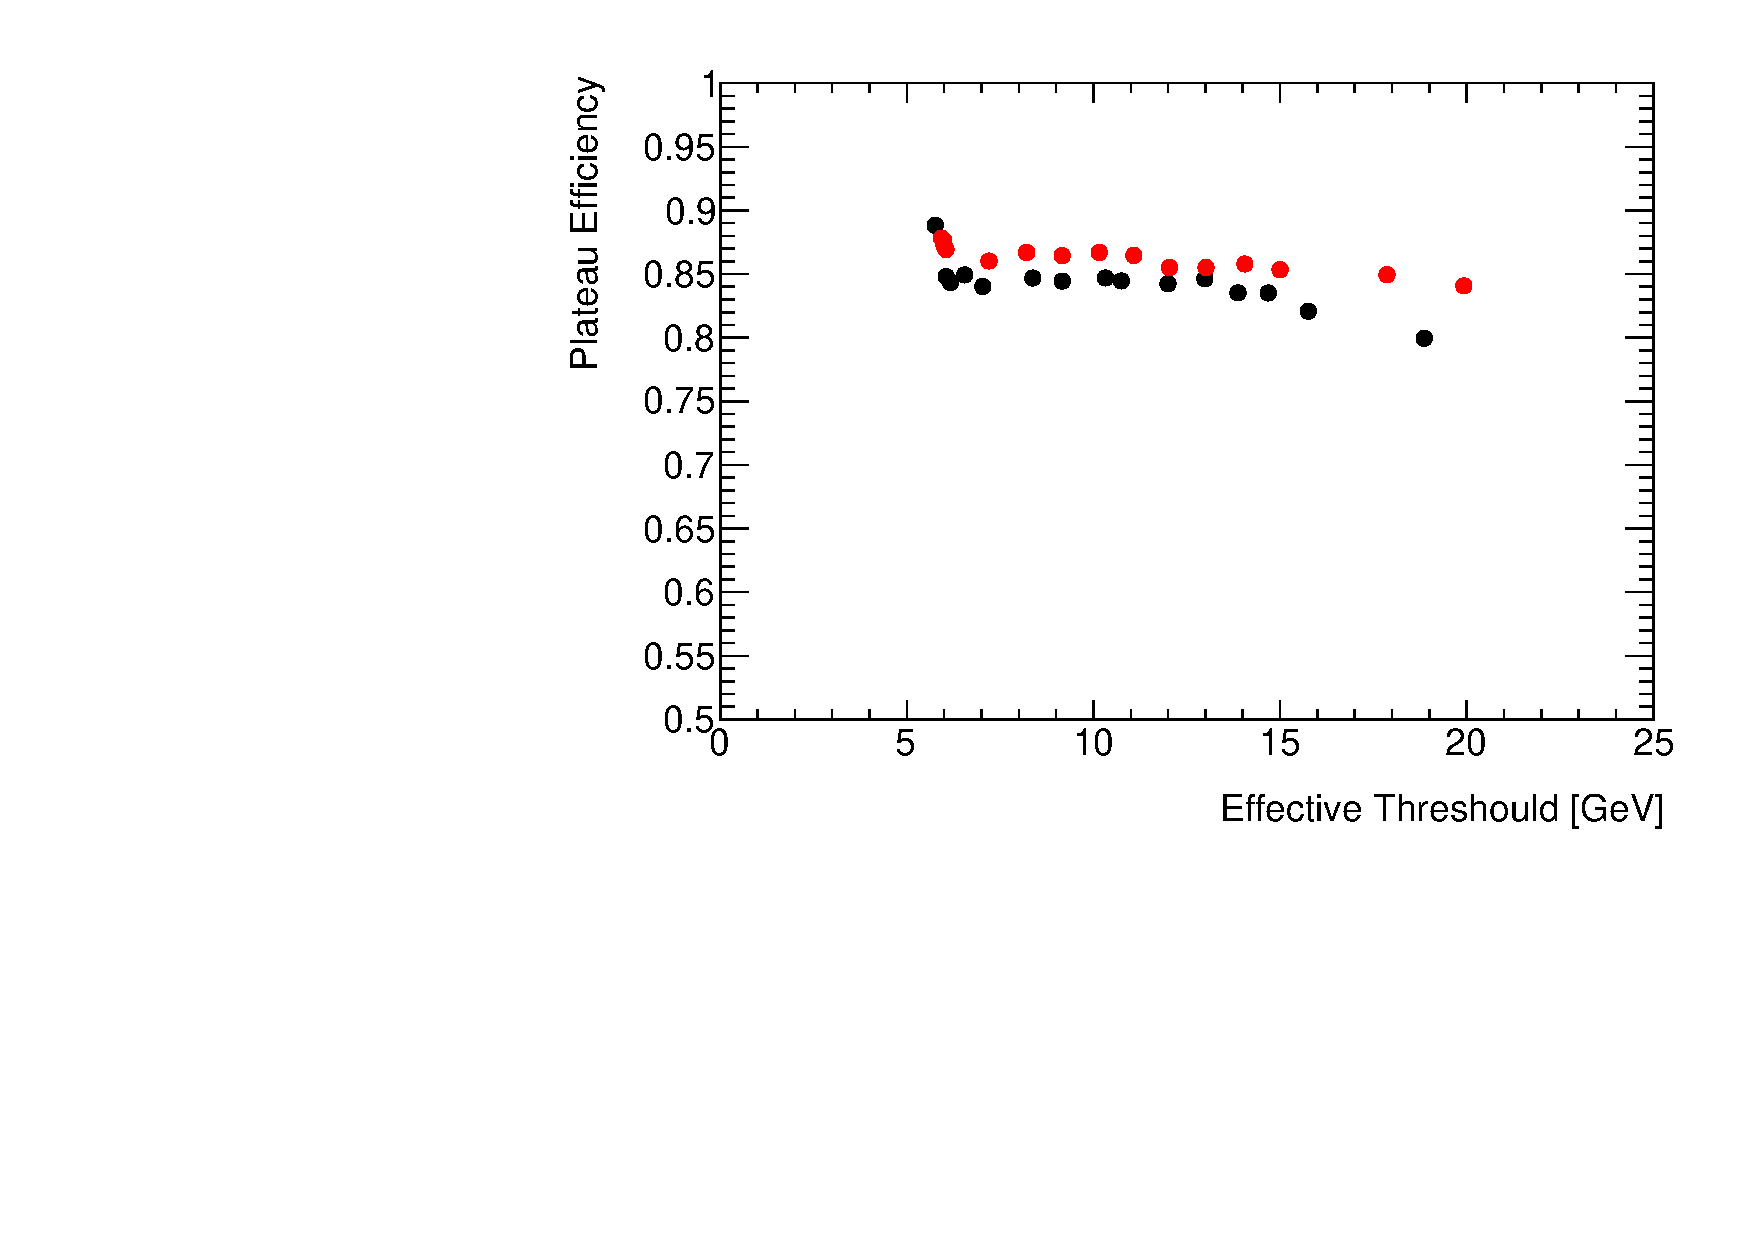
\includegraphics[clip, width=8cm]{fig/4/v05vsv06_Plateau.pdf}
        %\vspace{5pt}
        \subcaption{}
        \label{fig:Plateau_v06v05}
    \end{minipage}%
    \end{tabular}
    \caption{各$p_{\rm{T}}$閾値におけるTurn-on curveのPlateau EfficiencyにおけるResolutionの比較。(a):$\mathrm{CW_{Simu}}$と$\mathrm{CW_{2022}}$の比較。(b):$\mathrm{CW_{Data}}$と$\mathrm{CW_{2022}}$の比較。}
    \label{fig:Resolution_v07v06v05}
\end{figure}

\subsubsection{$p_{\rm{T}}^{offline}$分解能の評価}\label{分解能の評価}
$p_{\rm{T}}$分解能を式~\eqref{equ:residual}で計算する$p_{\rm{T}}$ residualを用いて評価する。
\begin{equation}
    p_{\rm{T}} residual = \frac{p_{\rm{T}}^{L1}-p_{\rm{T}}^{offline}}{p_{\rm{T}}^{offline}}
    \label{equ:residual}
\end{equation}
ここで、$p_{\rm{T}}^{L1}$はL1MuonでCWを用いて判定される$p_{\rm{T}}$閾値、$p_{\rm{T}}^{offline}$はオフライン再構成されたミューオンで$p_{\rm{T}}$ある。
そのため、$p_{\rm{T}}^{offline}$に対して正しく$p_{\rm{T}}^{L1}$を判定できていれば0に近づき、0から離れるほど$p_{\rm{T}}^{L1}$が$p_{\rm{T}}^{offline}$とずれていることになる。

この$p_{\rm{T}}$ residualを1~GeVごとの$p_{\rm{T}}^{offline}$に対して計算し、細かい$p_{\rm{T}}$に対する分解能を見る。
まず、本研究の手法で作成した$\mathrm{CW_{Simu}}$と2022年度Run-2で使用された$\mathrm{CW_{2022}}$の比較を行う。
評価にはシングルミューオンのシミュレーションサンプルを用いる。
図~\ref{residual_MC_3_10}と図~\ref{residual_MC_11_18}に1~GeVごとの$p_{\rm{T}}^{offline}$に対する$p_{\rm{T}}$ residual分布を示す。
本研究の手法で作成した$\mathrm{CW_{Simu}}$は、2022年度Run-3で使用された$\mathrm{CW_{2022}}$と同様の分布を示している。
\begin{figure}[htb]
  \centering
  %\rule{8cm}{6cm}
  \hspace*{-1cm}
  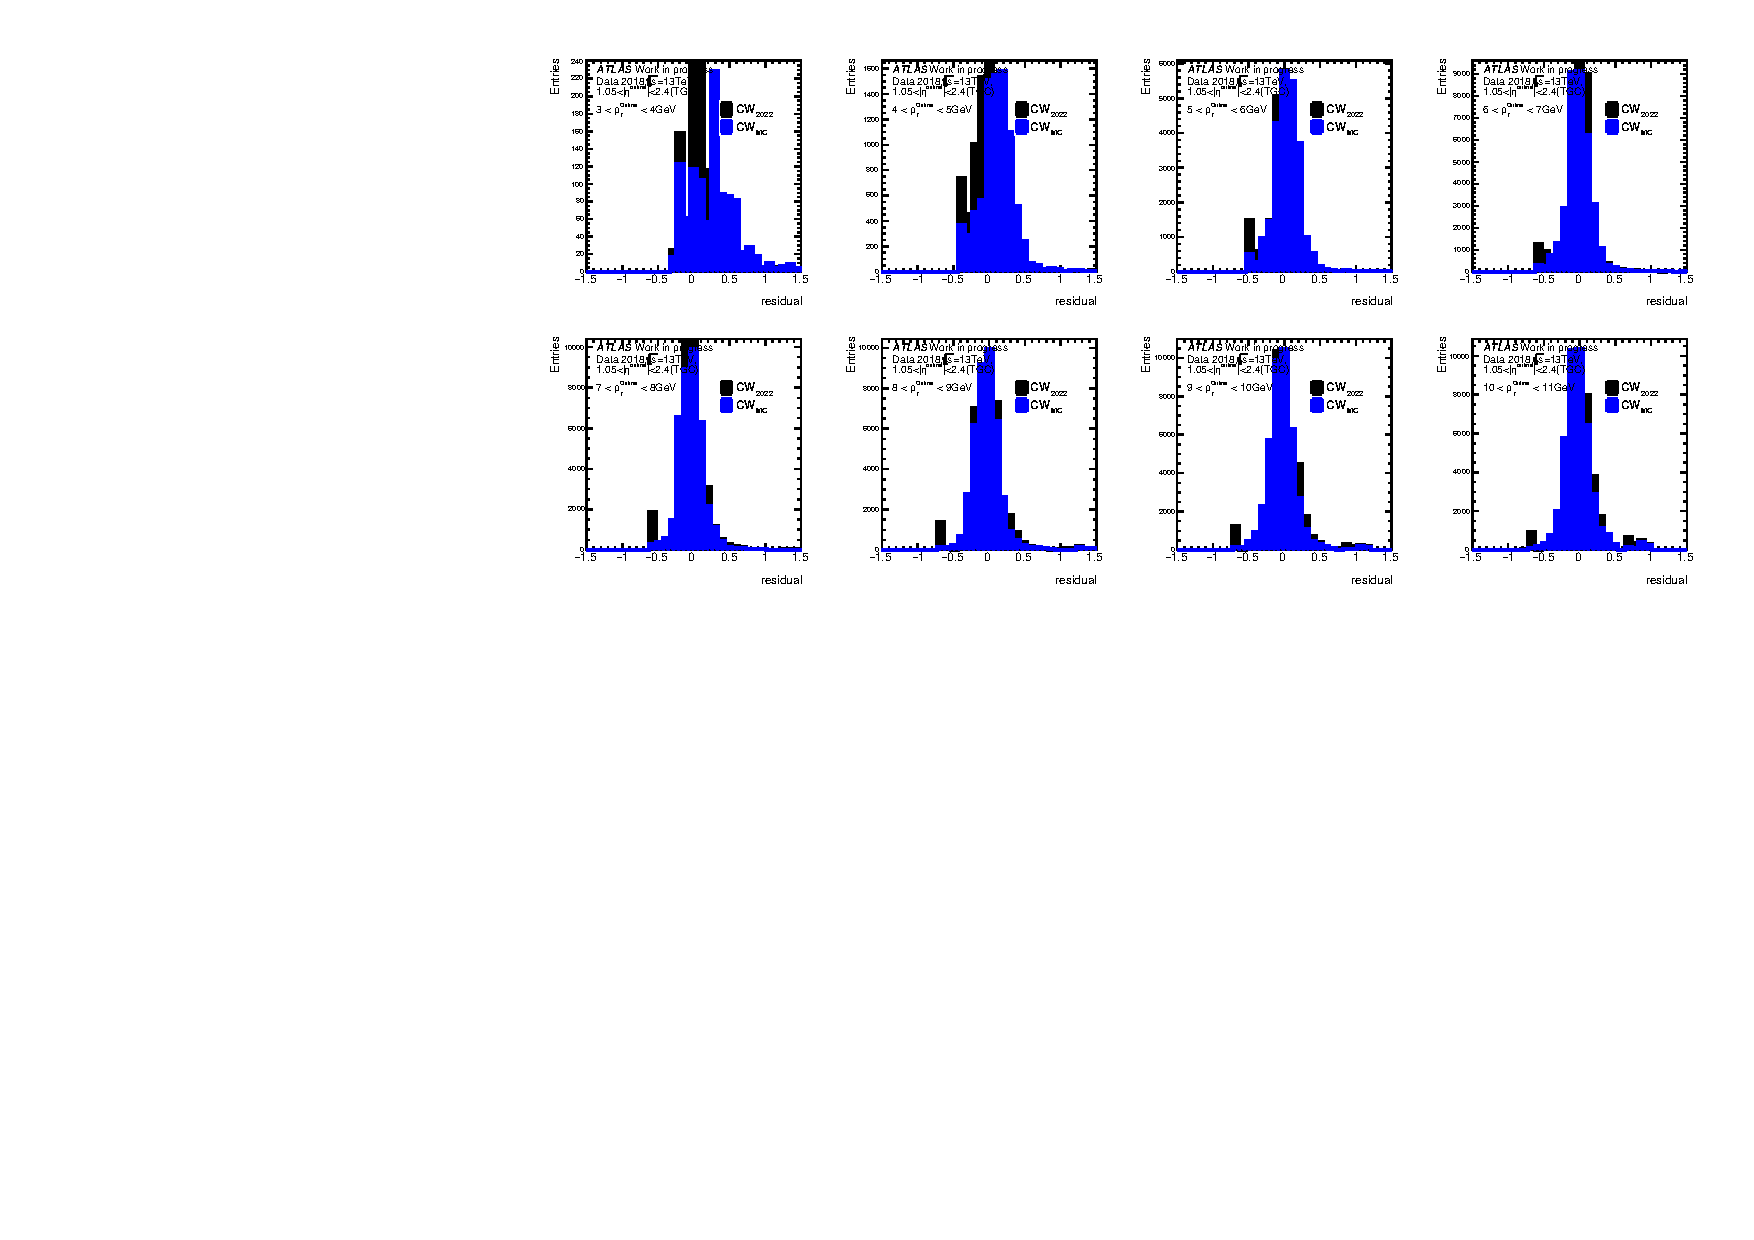
\includegraphics[clip, width=16cm]{fig/5/residual_MC_3_10.pdf}
  \caption{TGCにおける1GeV刻みのpT residual分布(3$\sim$10~GeV)。青が本研究の手法で作成した$\mathrm{CW_{Simu}}$を用いた結果、黒が2022年度Run-2で使用された$\mathrm{CW_{2022}}$を用いた結果である。}
  \label{residual_MC_3_10}
\end{figure}
\begin{figure}[htb]
  \centering
  %\rule{8cm}{6cm}
  \hspace*{-1cm}
  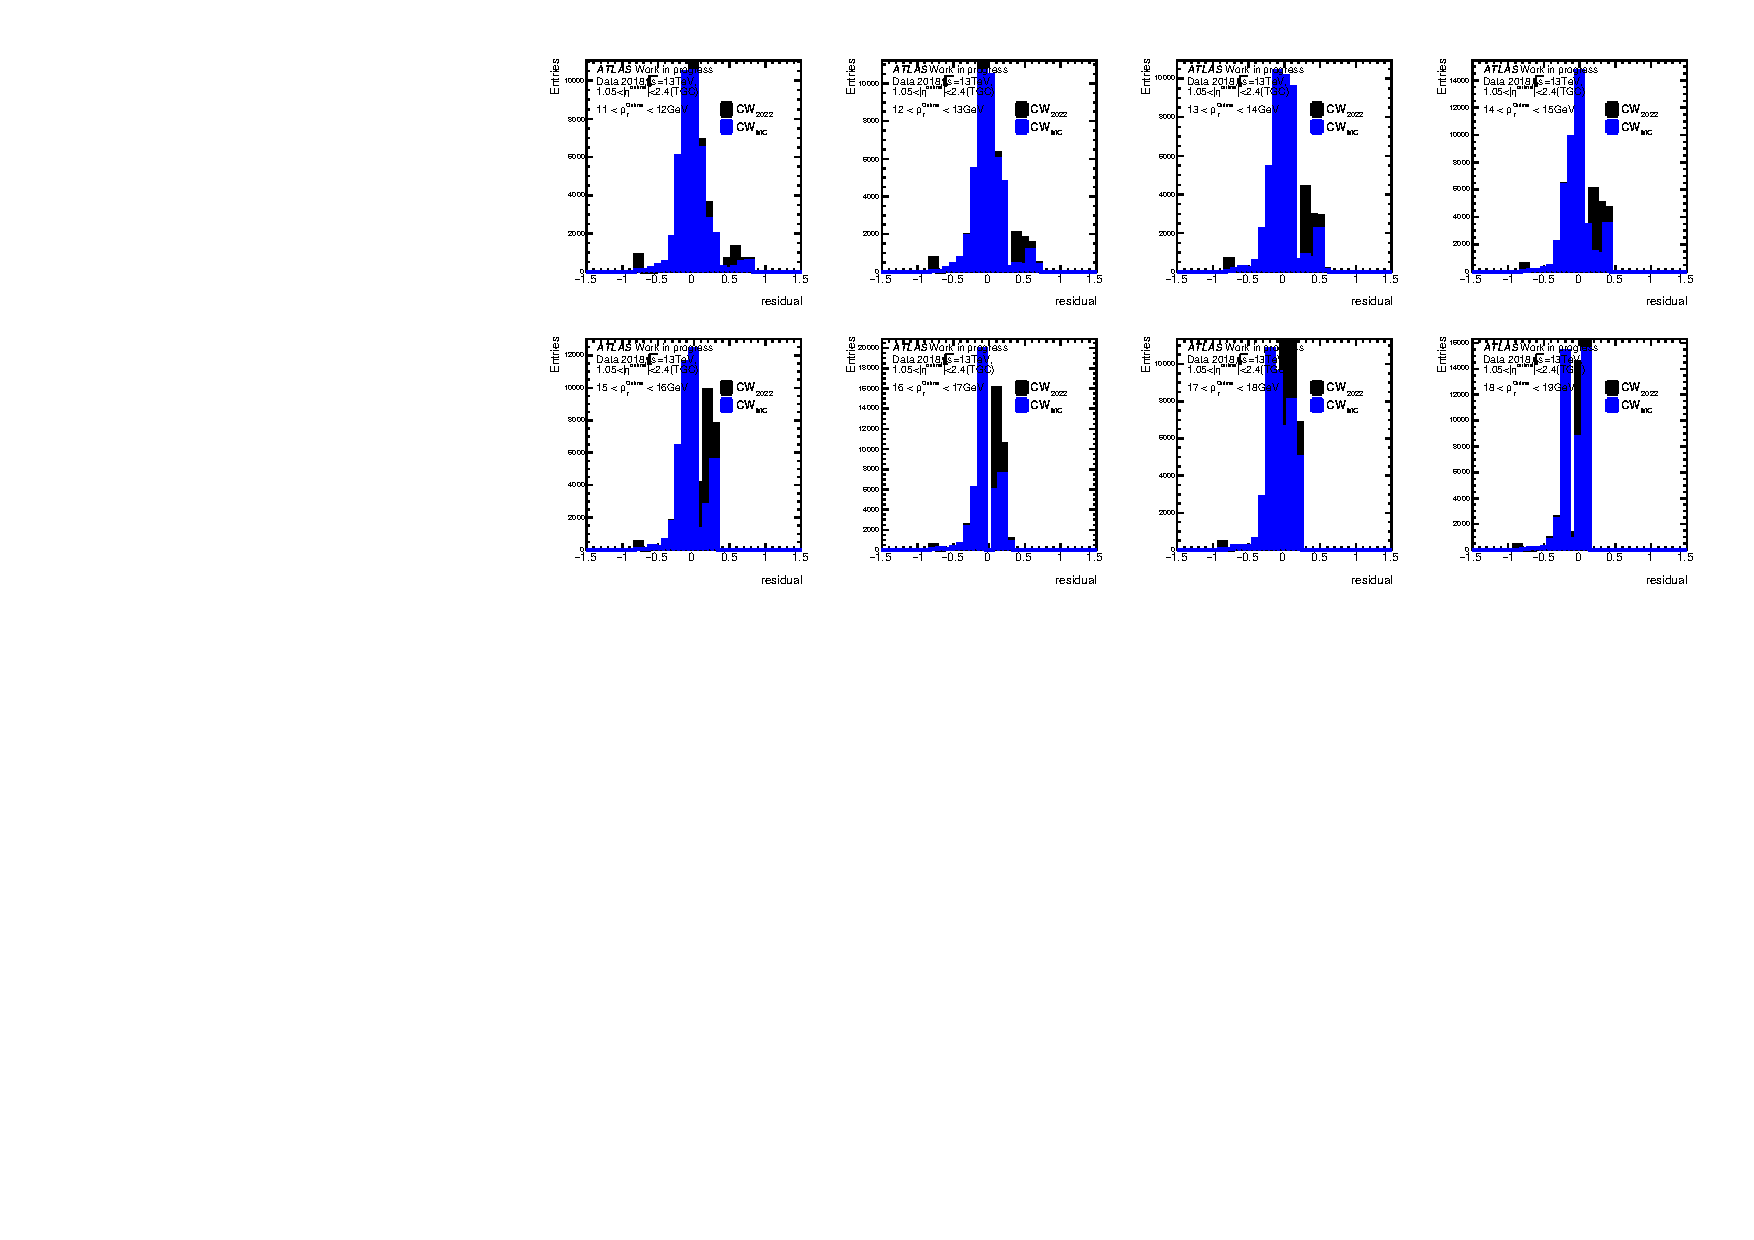
\includegraphics[clip, width=16cm]{fig/5/residual_MC_11_18.pdf}
  \caption{TGCにおける1GeV刻みのpT residual分布(11$\sim$18~GeV)。青が本研究の手法で作成した$\mathrm{CW_{Simu}}$を用いた結果、黒が2022年度Run-3で使用された$\mathrm{CW_{2022}}$を用いた結果である。}
  \label{residual_MC_11_18}
\end{figure}
図~\ref{residual_MC}には1GeV刻みの$p_{\rm{T}}$ residual分布のMean値と標準偏差を示した。
$\mathrm{CW_{2022}}$と比べ$\mathrm{CW_{Simu}}$は同程度のパフォーマンスが得られることが確認できる。一方で低い$p_{\rm{T}}$に対する$p_{\rm{T}}^{offline}$分解能は$\mathrm{CW_{2022}}$と比べて悪くなっている。これは、$p_{\rm{T}}$閾値の選択方法の影響が表れている。$\mathrm{CW_{2022}}$を作成した先行研究では、この$p_{\rm{T}}^{offline}$分解能が向上するような$p_{\rm{T}}$閾値の選択方法を確立し、15段階の$p_{\rm{T}}$閾値を選んでいた。一方、本研究ではEffective Threshouldを$p_{\rm{T}}$閾値とする選択方法を取っていたため、$p_{\rm{T}}^{offline}$分解能を評価した時、$\mathrm{CW_{2022}}$よりも悪化してしまったと考えられる。
本研究において図~\ref{fig:resi_std_Simu}から、すべての$p_{\rm{T}}$において$\mathrm{CW_{2022}}$と同程度のResolutionを得られていることから、機械学習の出力からの$p_{\rm{T}}$閾値の選択方法を変えことで、$\mathrm{CW_{2022}}$と同じ$p_{\rm{T}}^{offline}$分解能を持つような$p_{\rm{T}}$閾値を設定できると見込まれる。


\begin{figure}
    %\centering
    \begin{tabular}{cc}
    \begin{minipage}[b]{0.45\hsize}
        %\centering
        \hspace*{-1cm}
        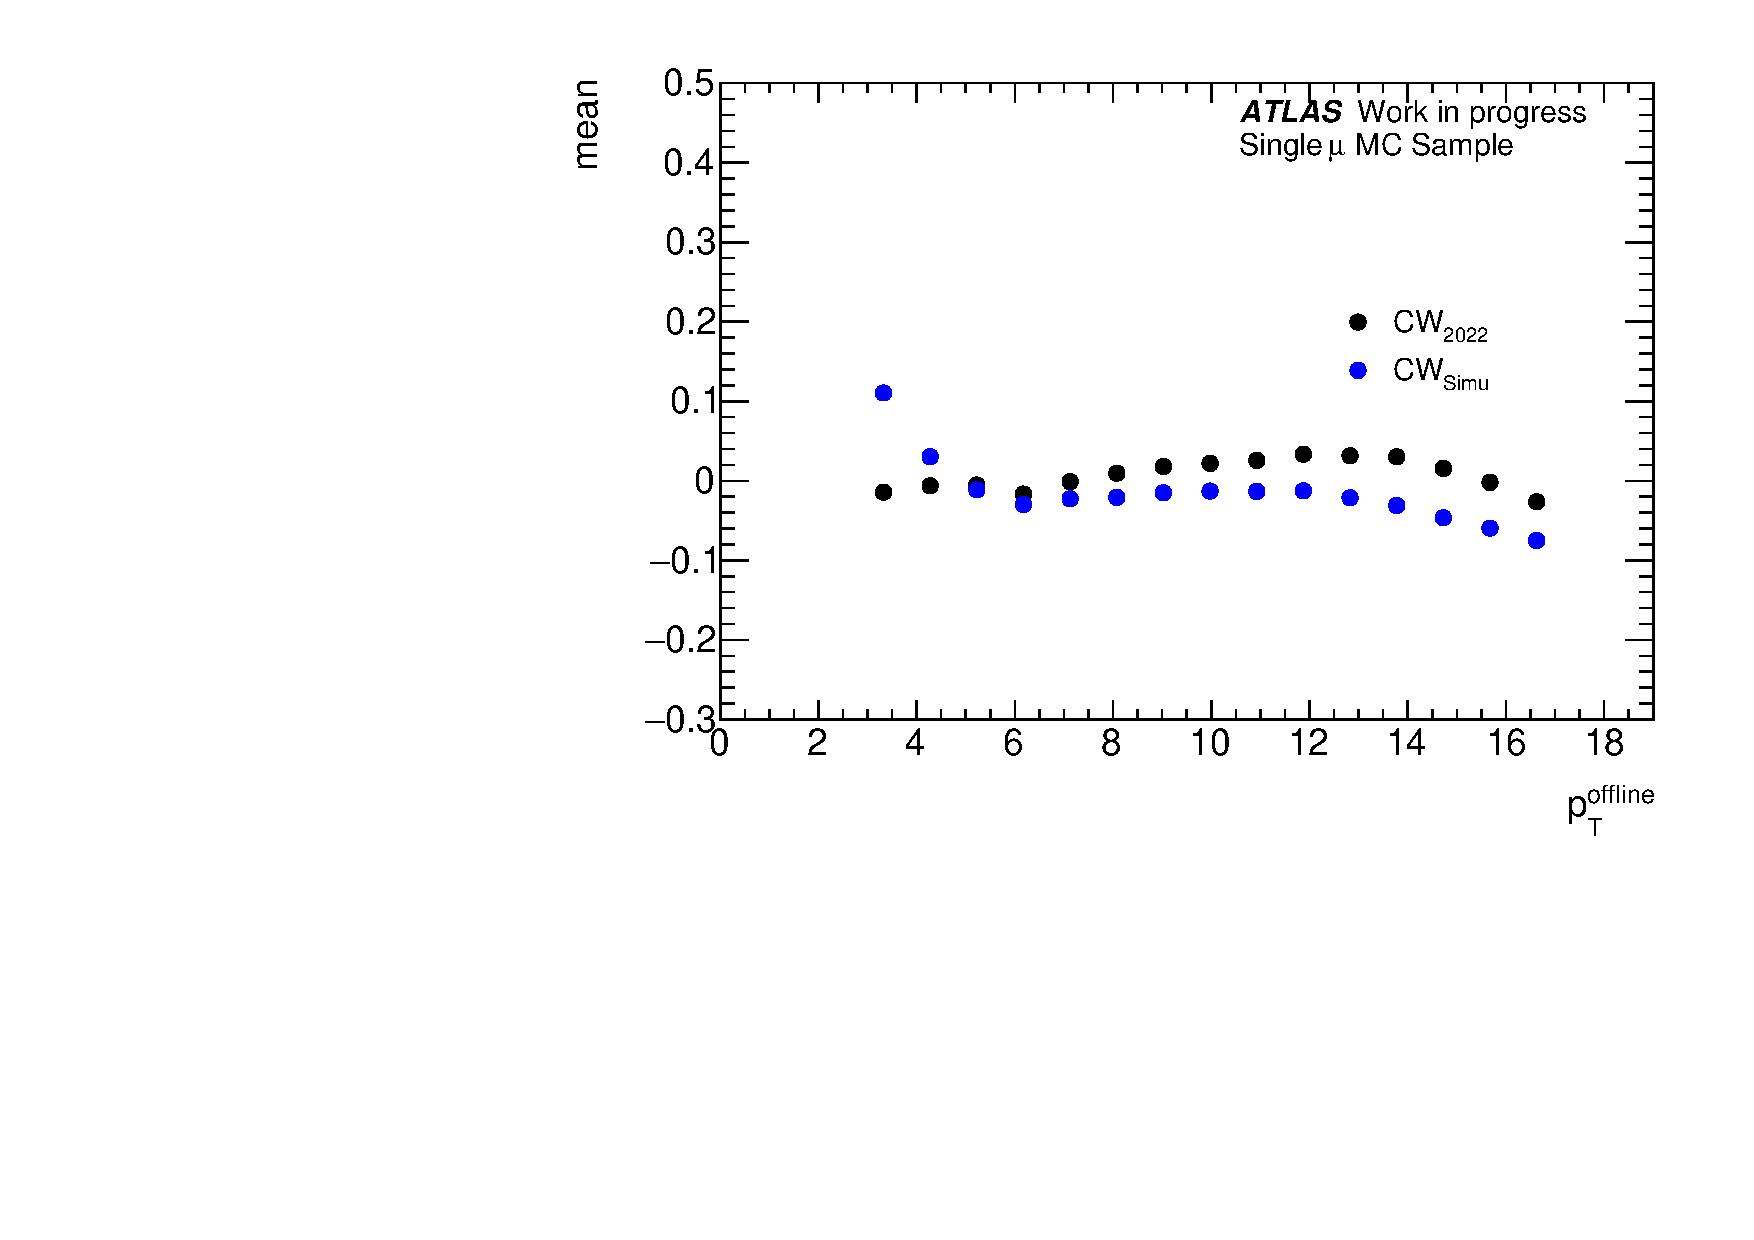
\includegraphics[clip, width=8cm]{fig/5/residual_mean_Simu.pdf}
        %\vspace{5pt}
        \subcaption{}
        \label{fig:resi_mean_Simu}
    \end{minipage}&
    %\hfill
    \begin{minipage}[b]{0.45\hsize}
        %\centering
        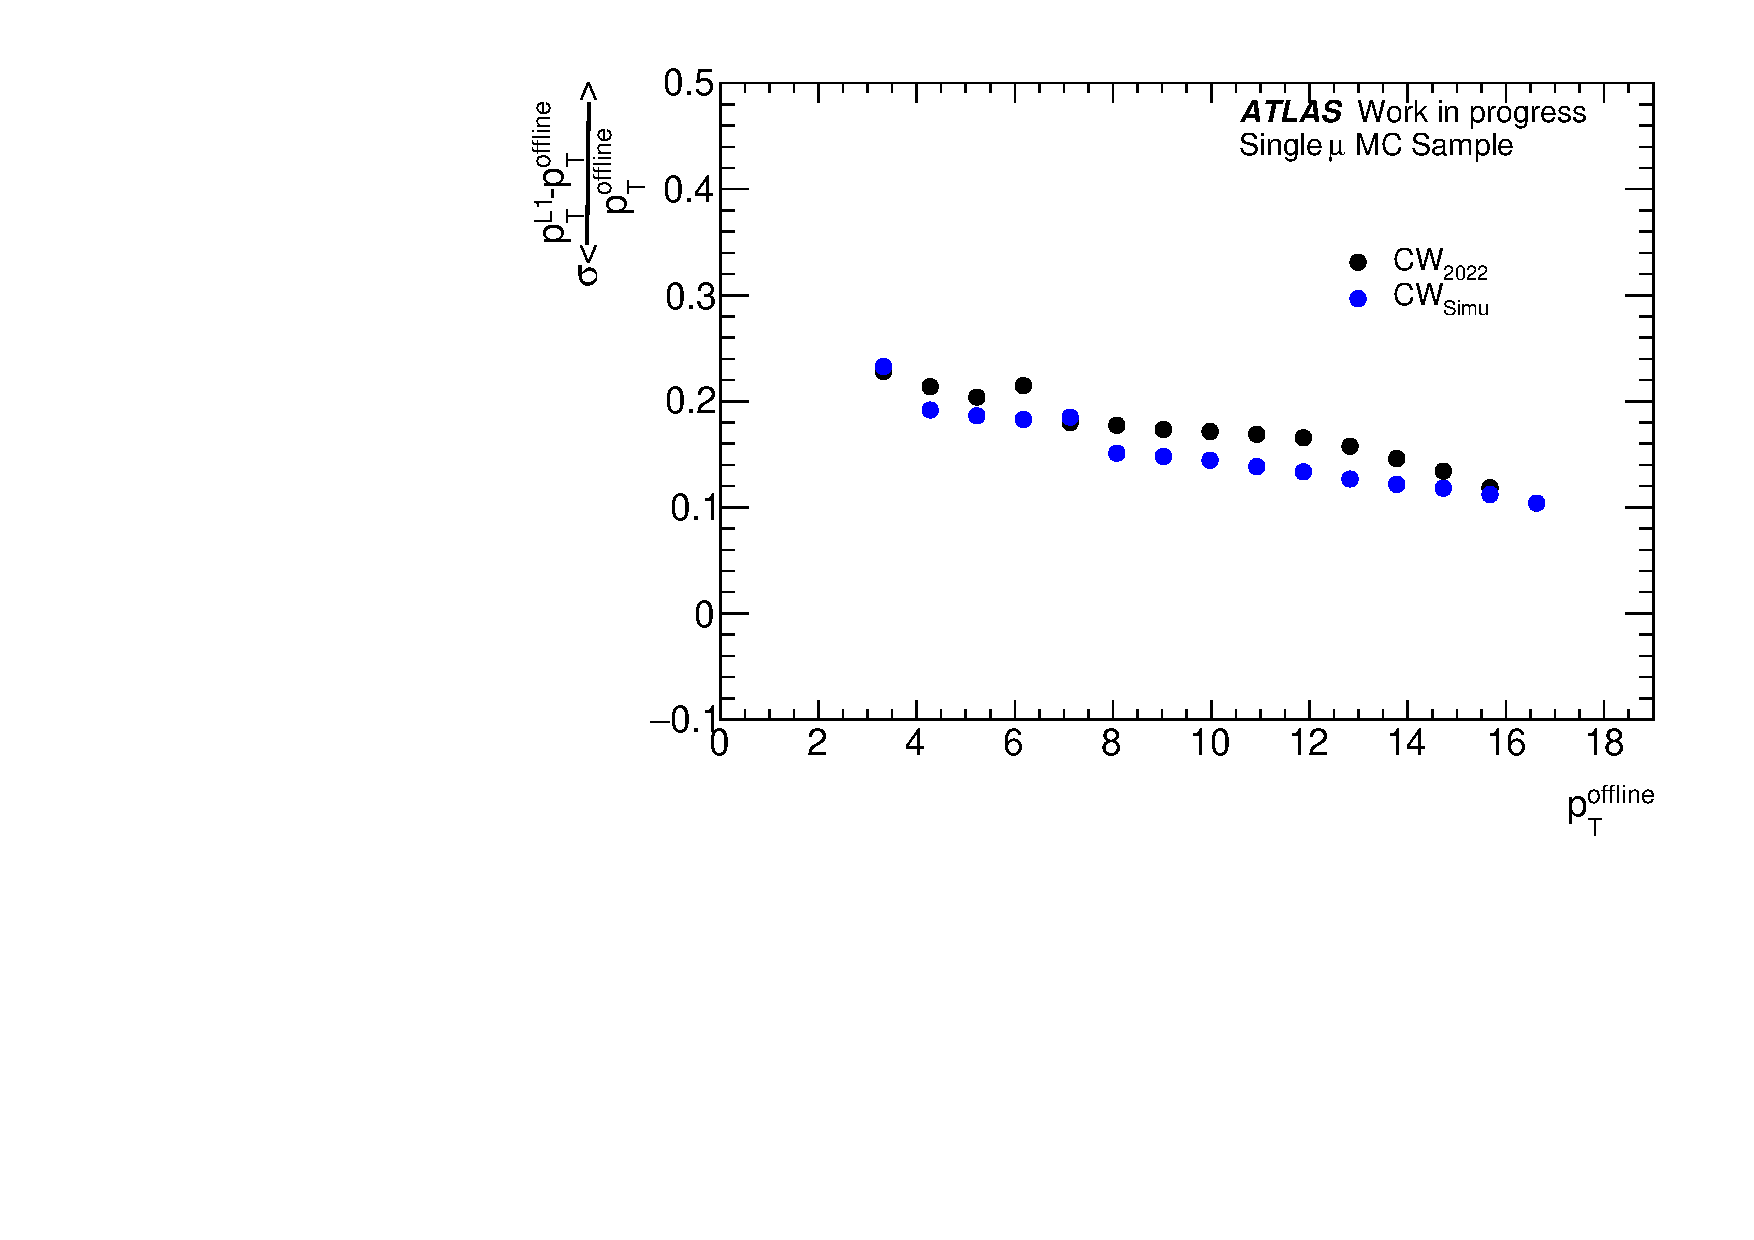
\includegraphics[clip, width=8cm]{fig/5/residual_stdDeVpdf_MC.pdf}
        %\vspace{5pt}
        \subcaption{}
        \label{fig:resi_std_Simu}
    \end{minipage}
    \end{tabular}
    \caption{本研究の手法で作成した$\mathrm{CW_{Simu}}$と2022年度Run-2で使用された$\mathrm{CW_{2022}}$の$p_{\rm{T}}$ residualの(左)Mean値と(右)標準偏差の比較。}
    \label{residual_MC}
\end{figure}

次に、本研究の手法で作成した$\mathrm{CW_{Data}}$と2022年度Run-2で使用された$\mathrm{CW_{2022}}$の比較を行う。
評価には2022年Run-2のデータを用いる。
図~\ref{residual_Data_3_10}と図~\ref{residual_Data_11_18}に1~GeVごとの$p_{\rm{T}}^{offline}$に対する$p_{\rm{T}}$ residual分布を示す。
本研究の手法で作成した$\mathrm{CW_{Data}}$は、2022年度Run-2で使用された$\mathrm{CW_{2022}}$と比べて$p_{\rm{T}}^{offline}$分解能のmean値が悪くなっているが、Resolutionを比べると改善されていることから、$\mathrm{CW_{Simu}}$の評価で述べたように、機械学習の出力からの$p_{\rm{T}}$閾値の選択方法によってmean値においても改善が見込まれる。


\begin{figure}[htb]
  \centering
  %\rule{8cm}{6cm}
  \hspace*{-1cm}
  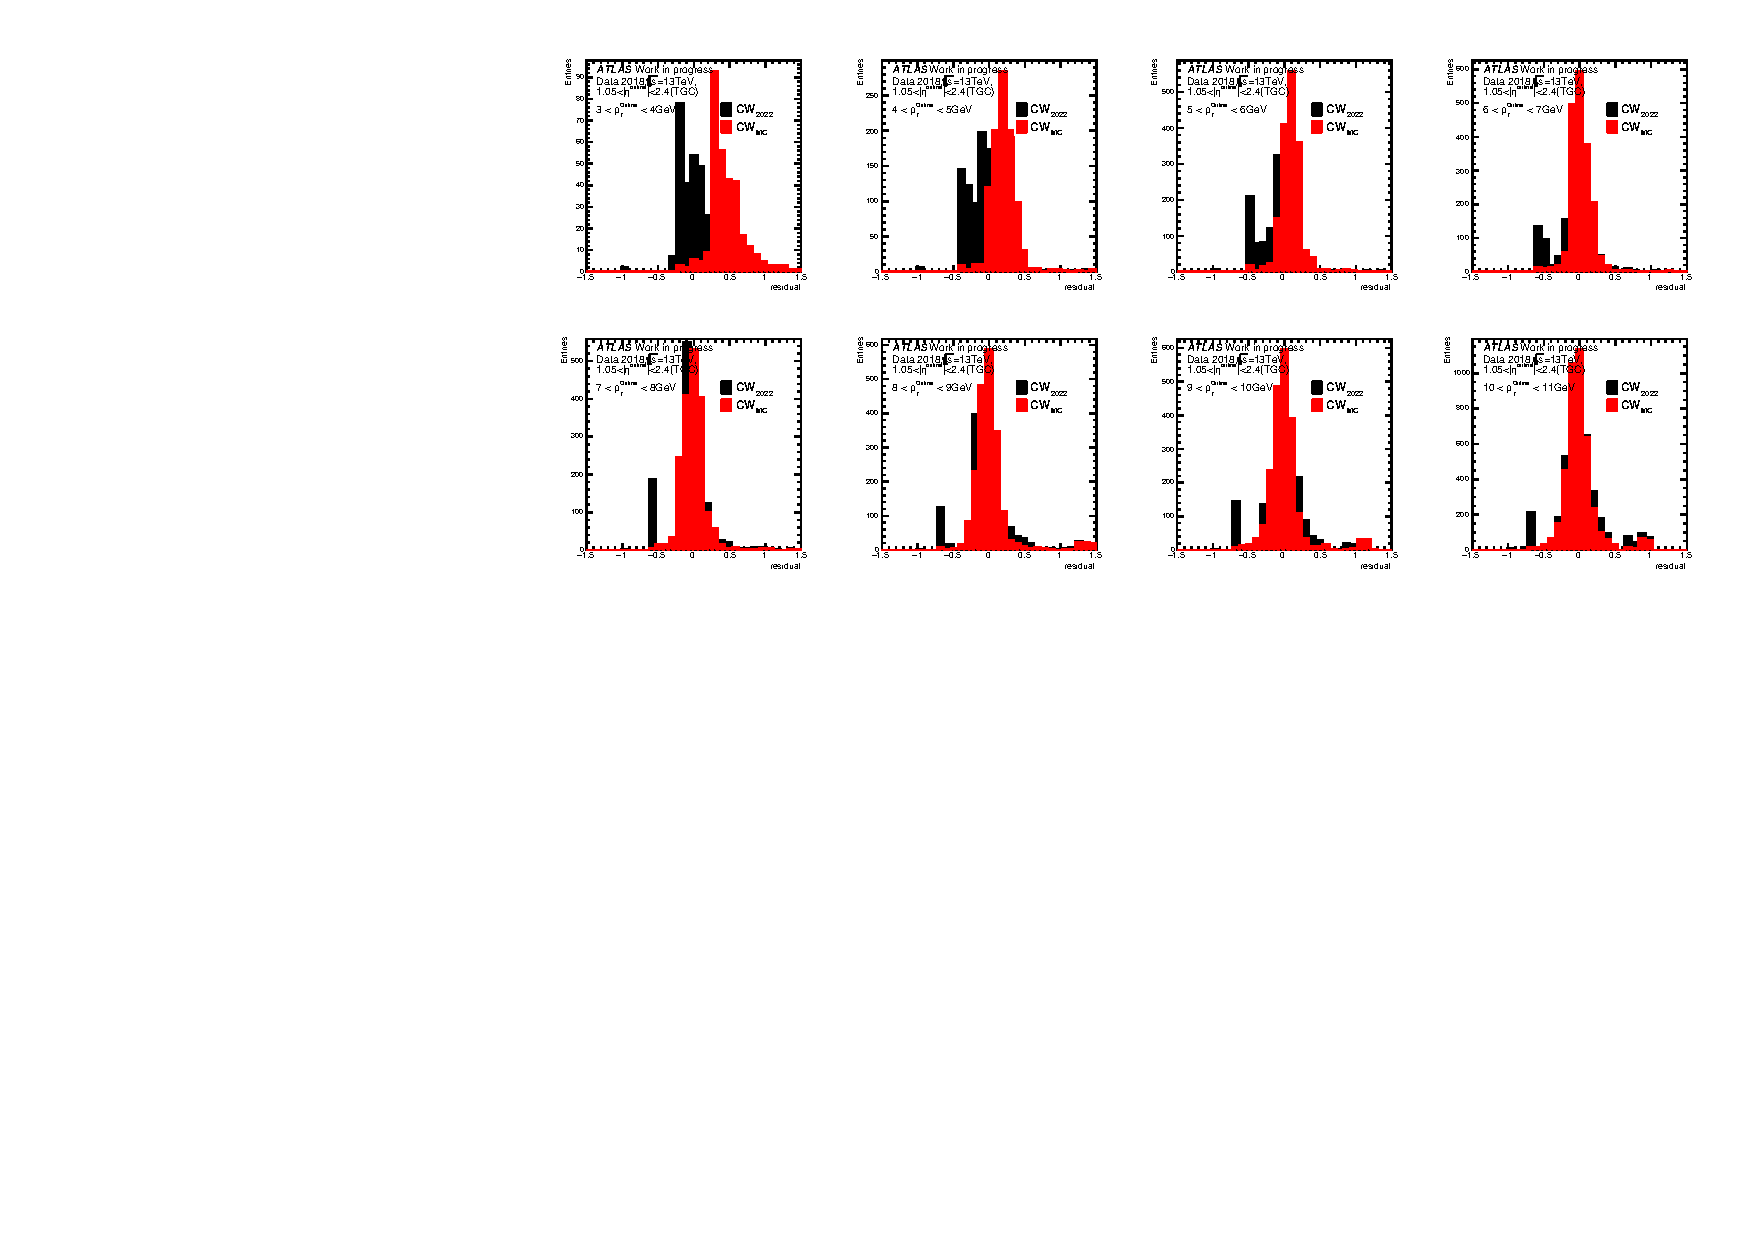
\includegraphics[clip, width=16cm]{fig/5/residual_Data_3_10.pdf}
  \caption{TGCにおける1GeV刻みのpT residual分布(3$\sim$10~GeV)。赤が本研究の手法で作成した$\mathrm{CW_{Data}}$を用いた結果、黒が2022年度Run-2で使用された$\mathrm{CW_{2022}}$を用いた結果である。}
  \label{residual_Data_3_10}
\end{figure}
\begin{figure}[htb]
  \centering
  %\rule{8cm}{6cm}
  \hspace*{-1cm}
  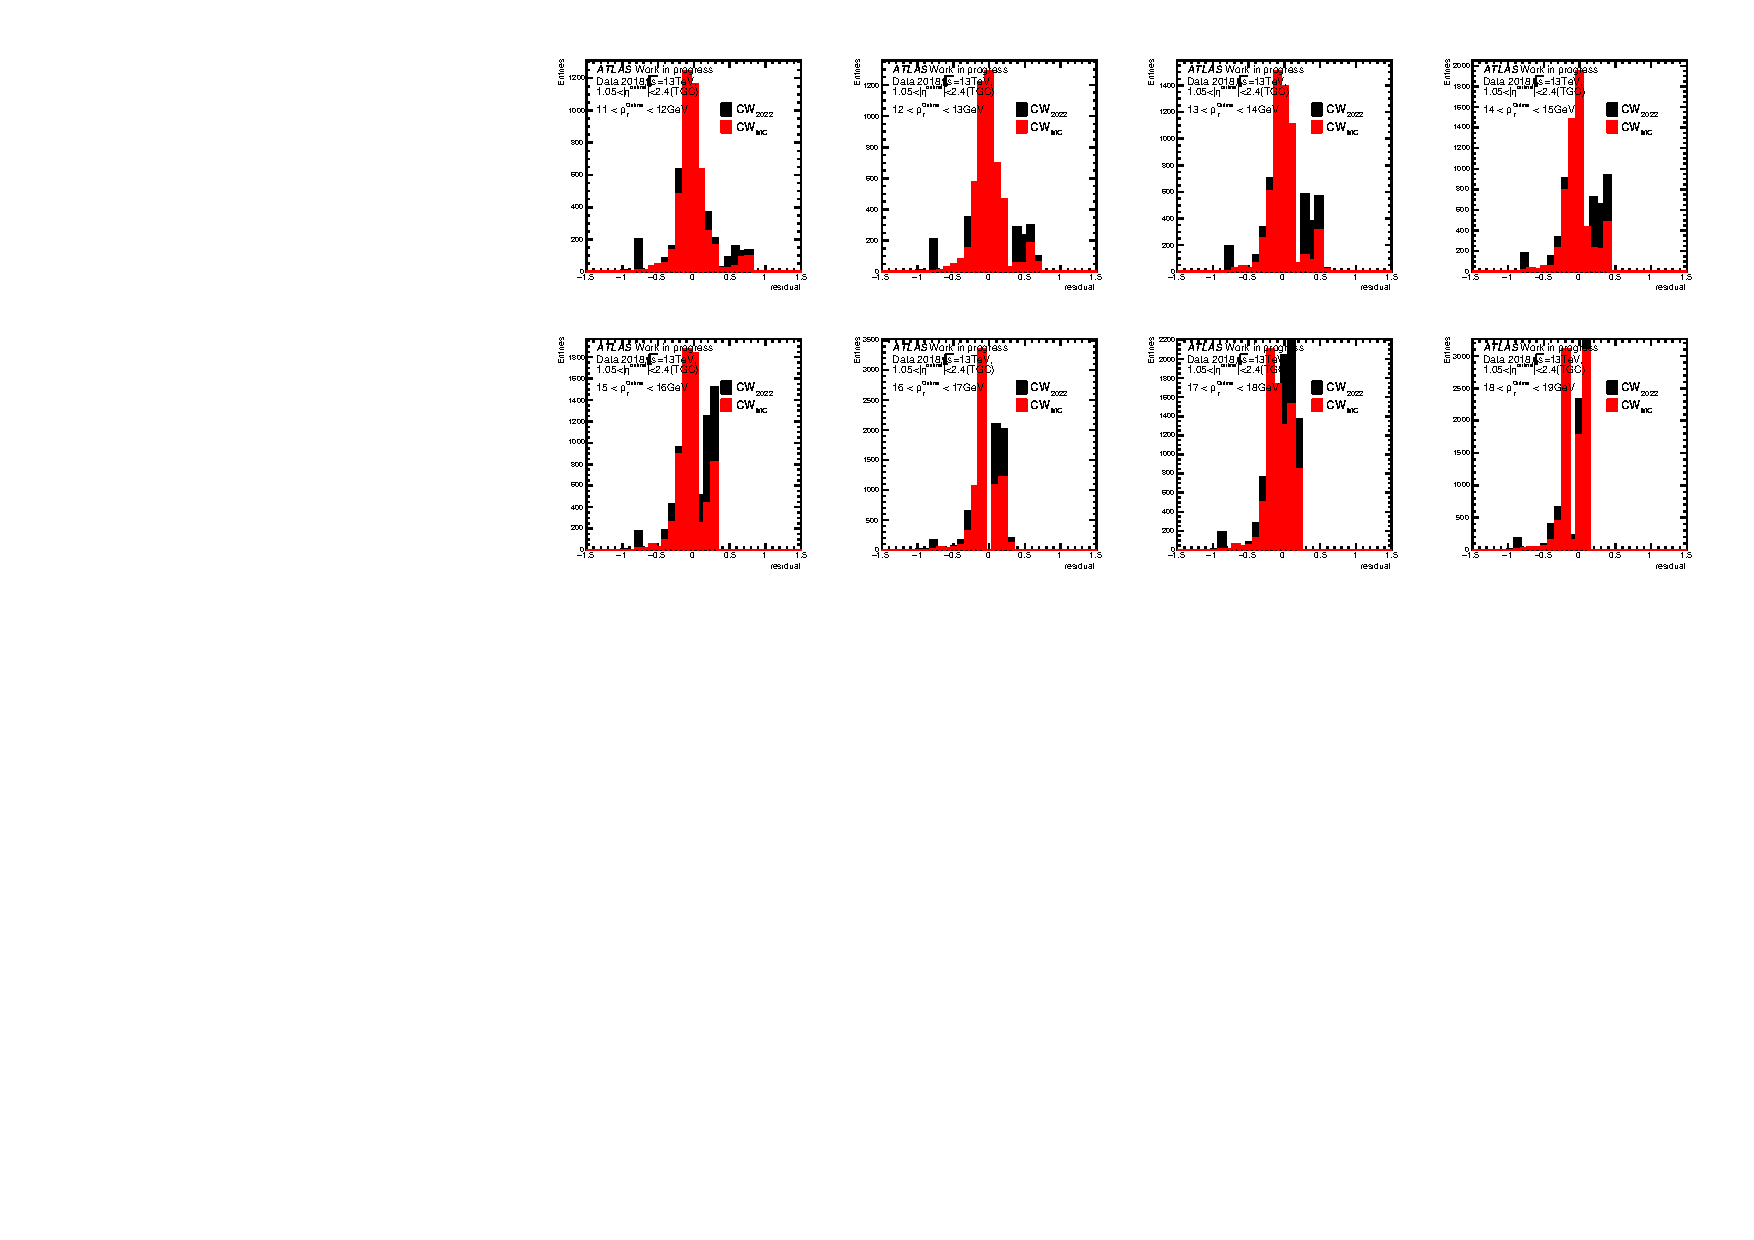
\includegraphics[clip, width=16cm]{fig/5/residual_Data_11_18.pdf}
  \caption{TGCにおける1GeV刻みのpT residual分布(11$\sim$18~GeV)。赤が本研究の手法で作成した$\mathrm{CW_{Data}}$を用いた結果、黒が2022年度Run-2で使用された$\mathrm{CW_{2022}}$を用いた結果である。}
  \label{residual_Data_11_18}
\end{figure}
図~\ref{residual_MC}には1GeV刻みの$p_{\rm{T}}$ residual分布のMean値と標準偏差を示した。
\begin{figure}
    %\centering
    \begin{tabular}{cc}
    \begin{minipage}[b]{0.45\hsize}
        %\centering
        \hspace*{-1cm}
        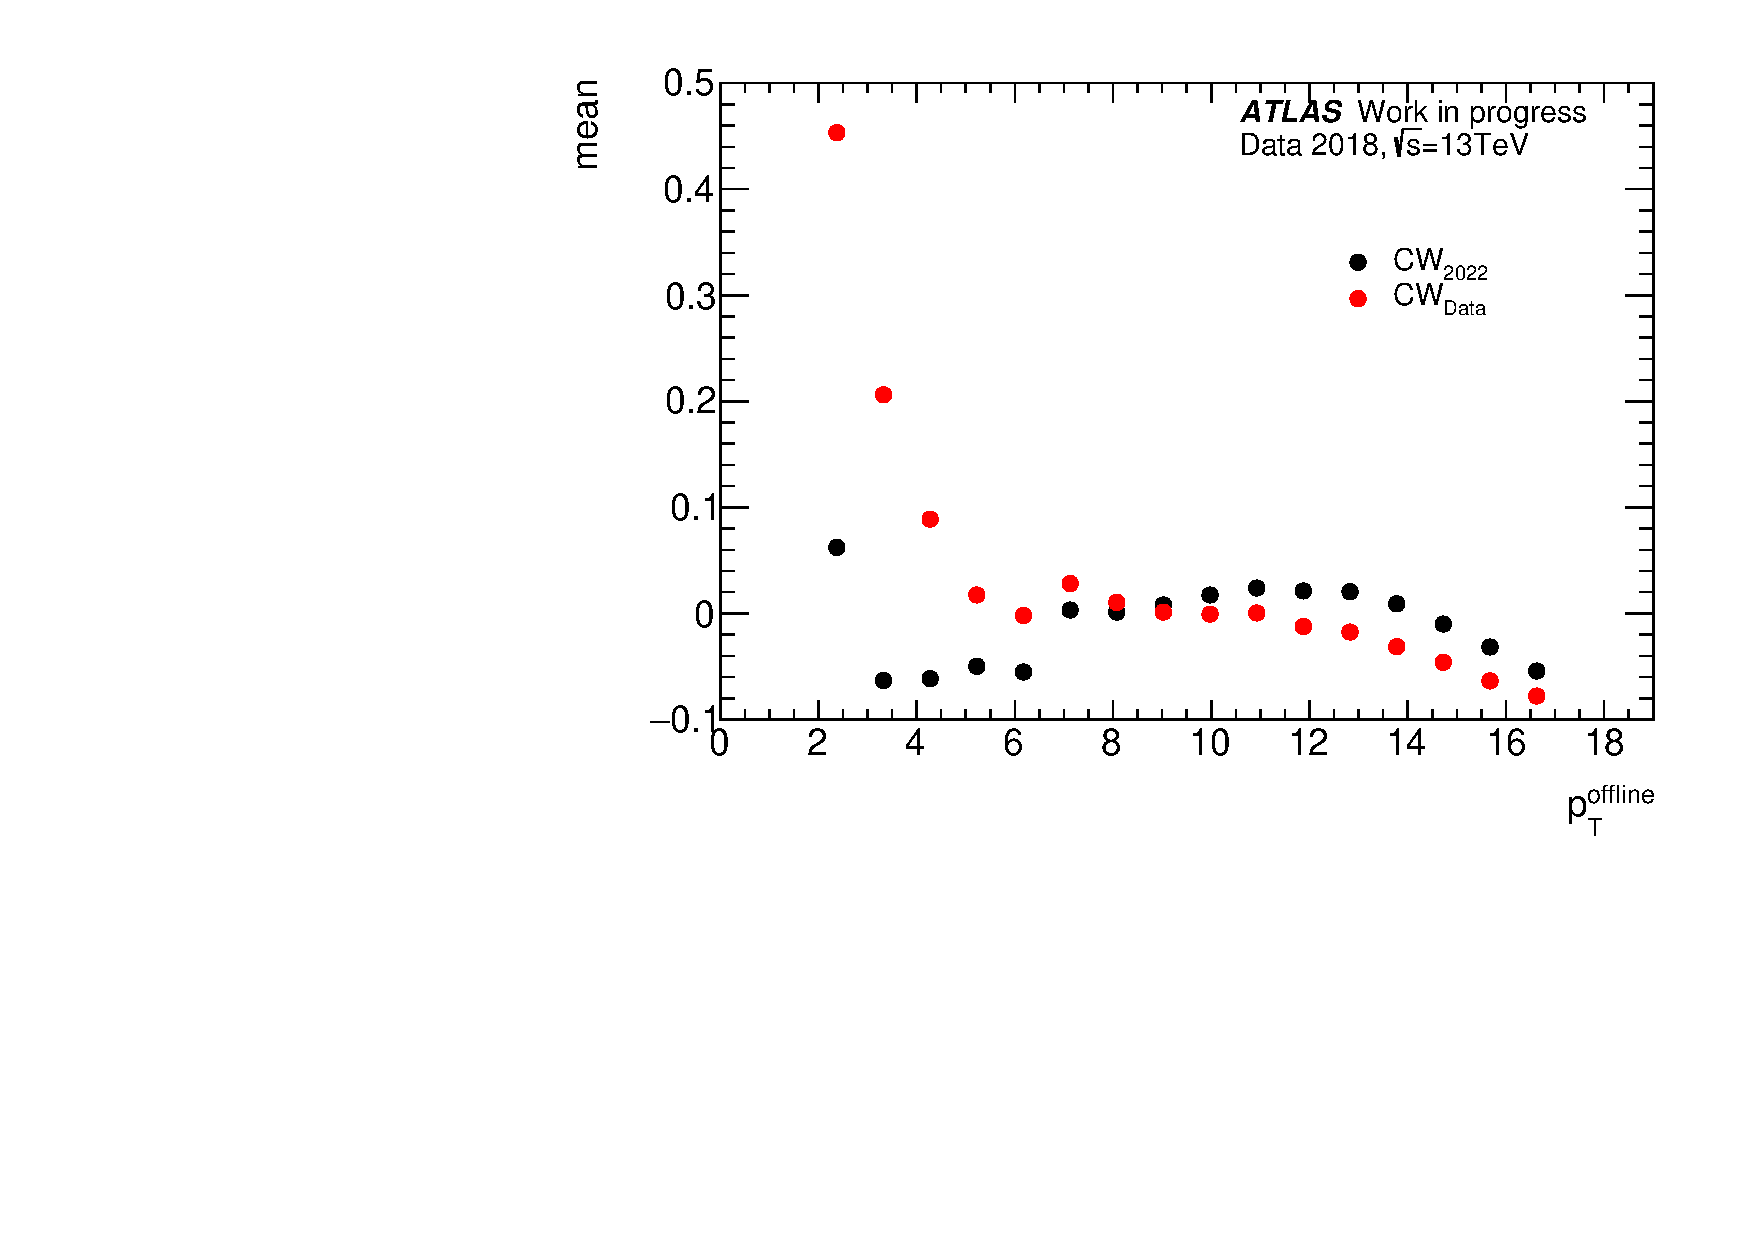
\includegraphics[clip, width=8cm]{fig/5/residual_mean_Data.pdf}
        %\vspace{5pt}
        \subcaption{}
        \label{fig:resi_mean_Data}
    \end{minipage}&
    %\hfill
    \begin{minipage}[b]{0.45\hsize}
        %\centering
        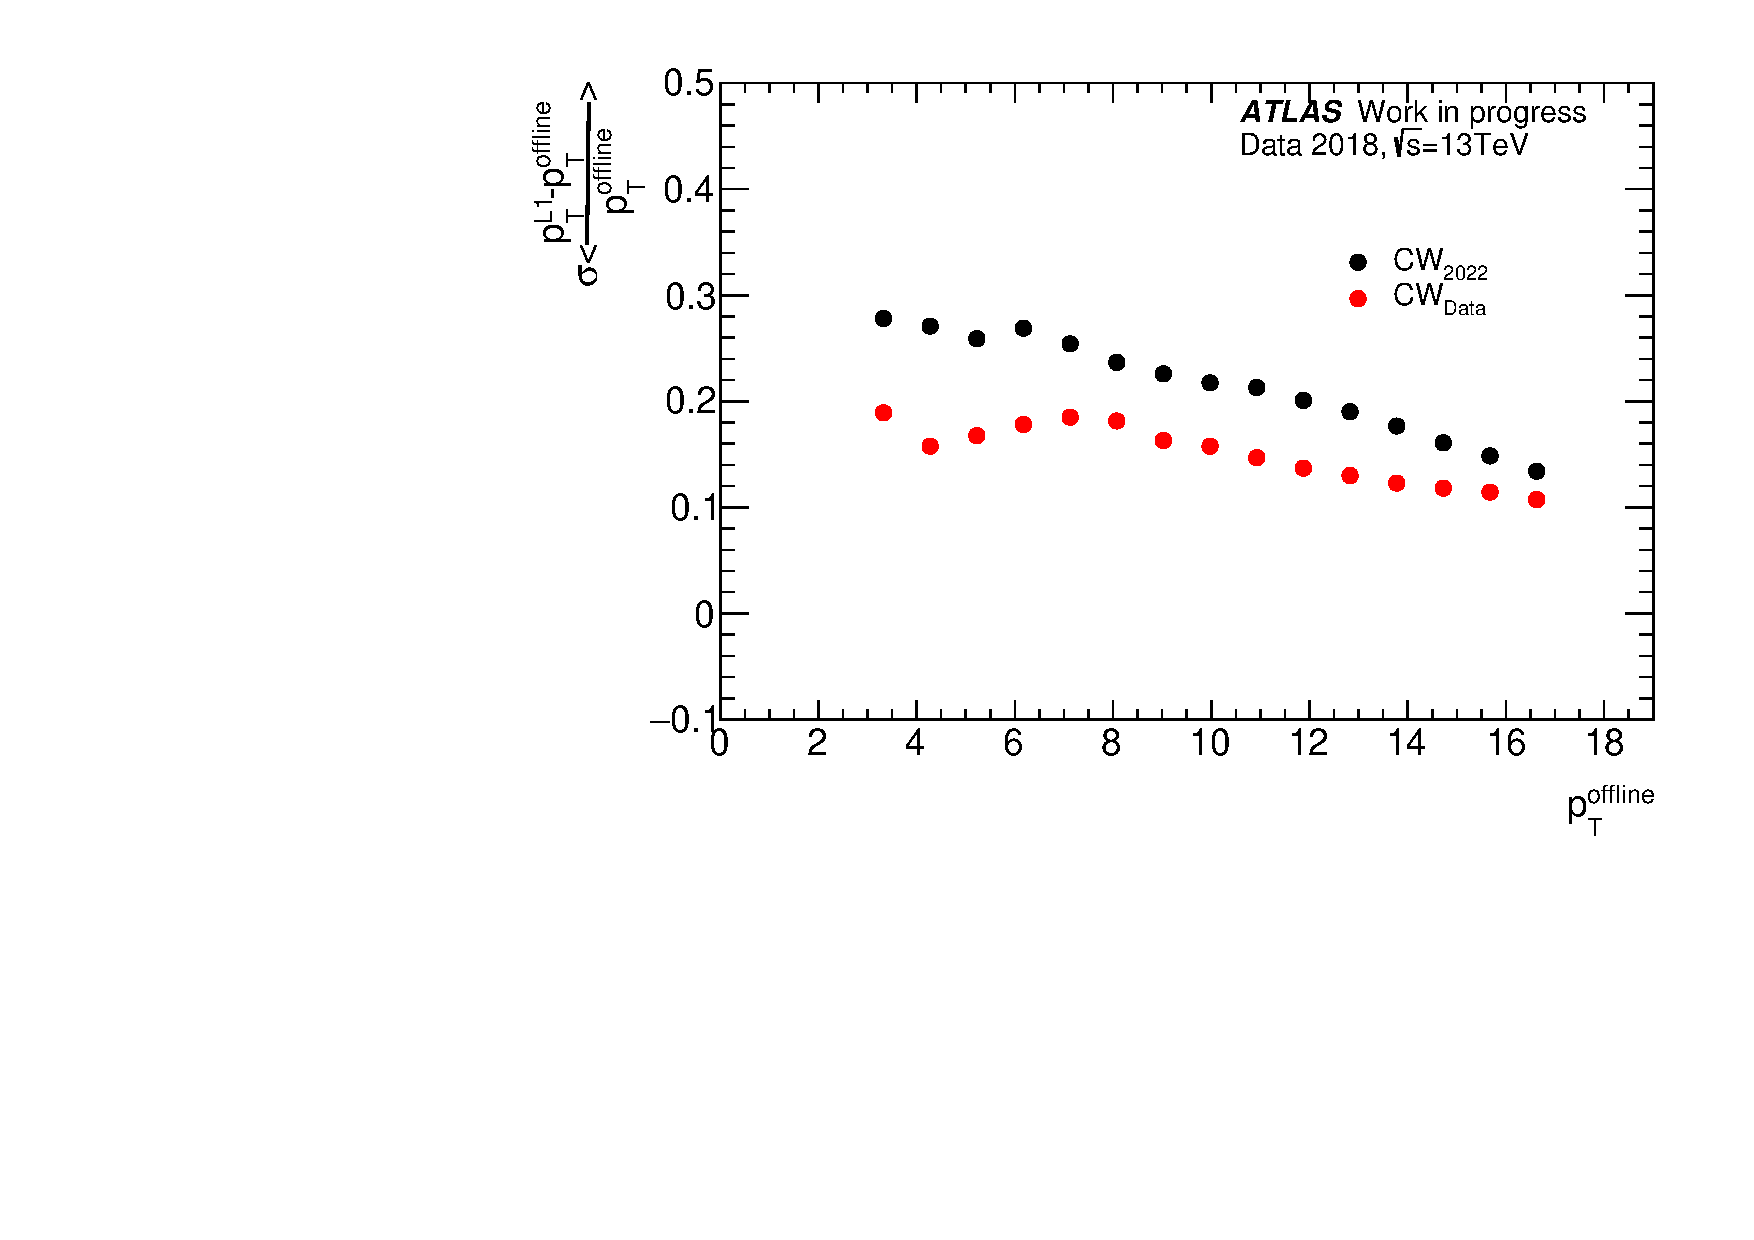
\includegraphics[clip, width=8cm]{fig/5/residual_stdDeVpdf.pdf}
        %\vspace{5pt}
        \subcaption{}
        \label{fig:resi_std_Data}
    \end{minipage}
    \end{tabular}
    \caption{本研究の手法で作成した$\mathrm{CW_{Data}}$と2022年度Run-2で使用された$\mathrm{CW_{2022}}$の$p_{\rm{T}}$ residualの(左)Mean値と(右)標準偏差の比較。}
    \label{residual_MC}
\end{figure}





\subsection{機械学習によるCWの最適化の評価}
実際のデータを機械学習に用いることで期待されるCWの最適化の効果について評価を行う。

本研究で開発した手法では、実際のデータをトレーニング用いることで自動で最適化を行うことで$\mathrm{CW_{Data}}$と$\mathrm{CW_{Simu}}$を作成した。そのため、最適化を行っていない$\mathrm{CW_{2022}}$よりもトリガー性能が向上することが期待される。

まず、検出器アライメントに対応してCWをズラすことができているかを確認する。
8回転対象の磁場構造において、同じ磁場構造となる場所に位置するRoIのCWの、$p_{\rm{T}}$閾値が14~GeVとなる領域についての$\mathrm{CW_{Data}}$と$\mathrm{CW_{2022}}$の比較を図~\ref{fig:CWv05v07}に示す。
図~\ref{fig:CWv05v07}に示す8個のCWは、シミュレーション上では磁場構造が同じになるため、黒枠で表される$\mathrm{CW_{2022}}$はすべて同じ形である。しかし、\ref{ズレ}節で述べたように、実際の検出器のズレによって場所によって磁場構造が異なるため、本手法で作成した$\mathrm{CW_{Data}}$ではCWに数マス分のズレが生じている。
\begin{figure}[tb]
  \centering
  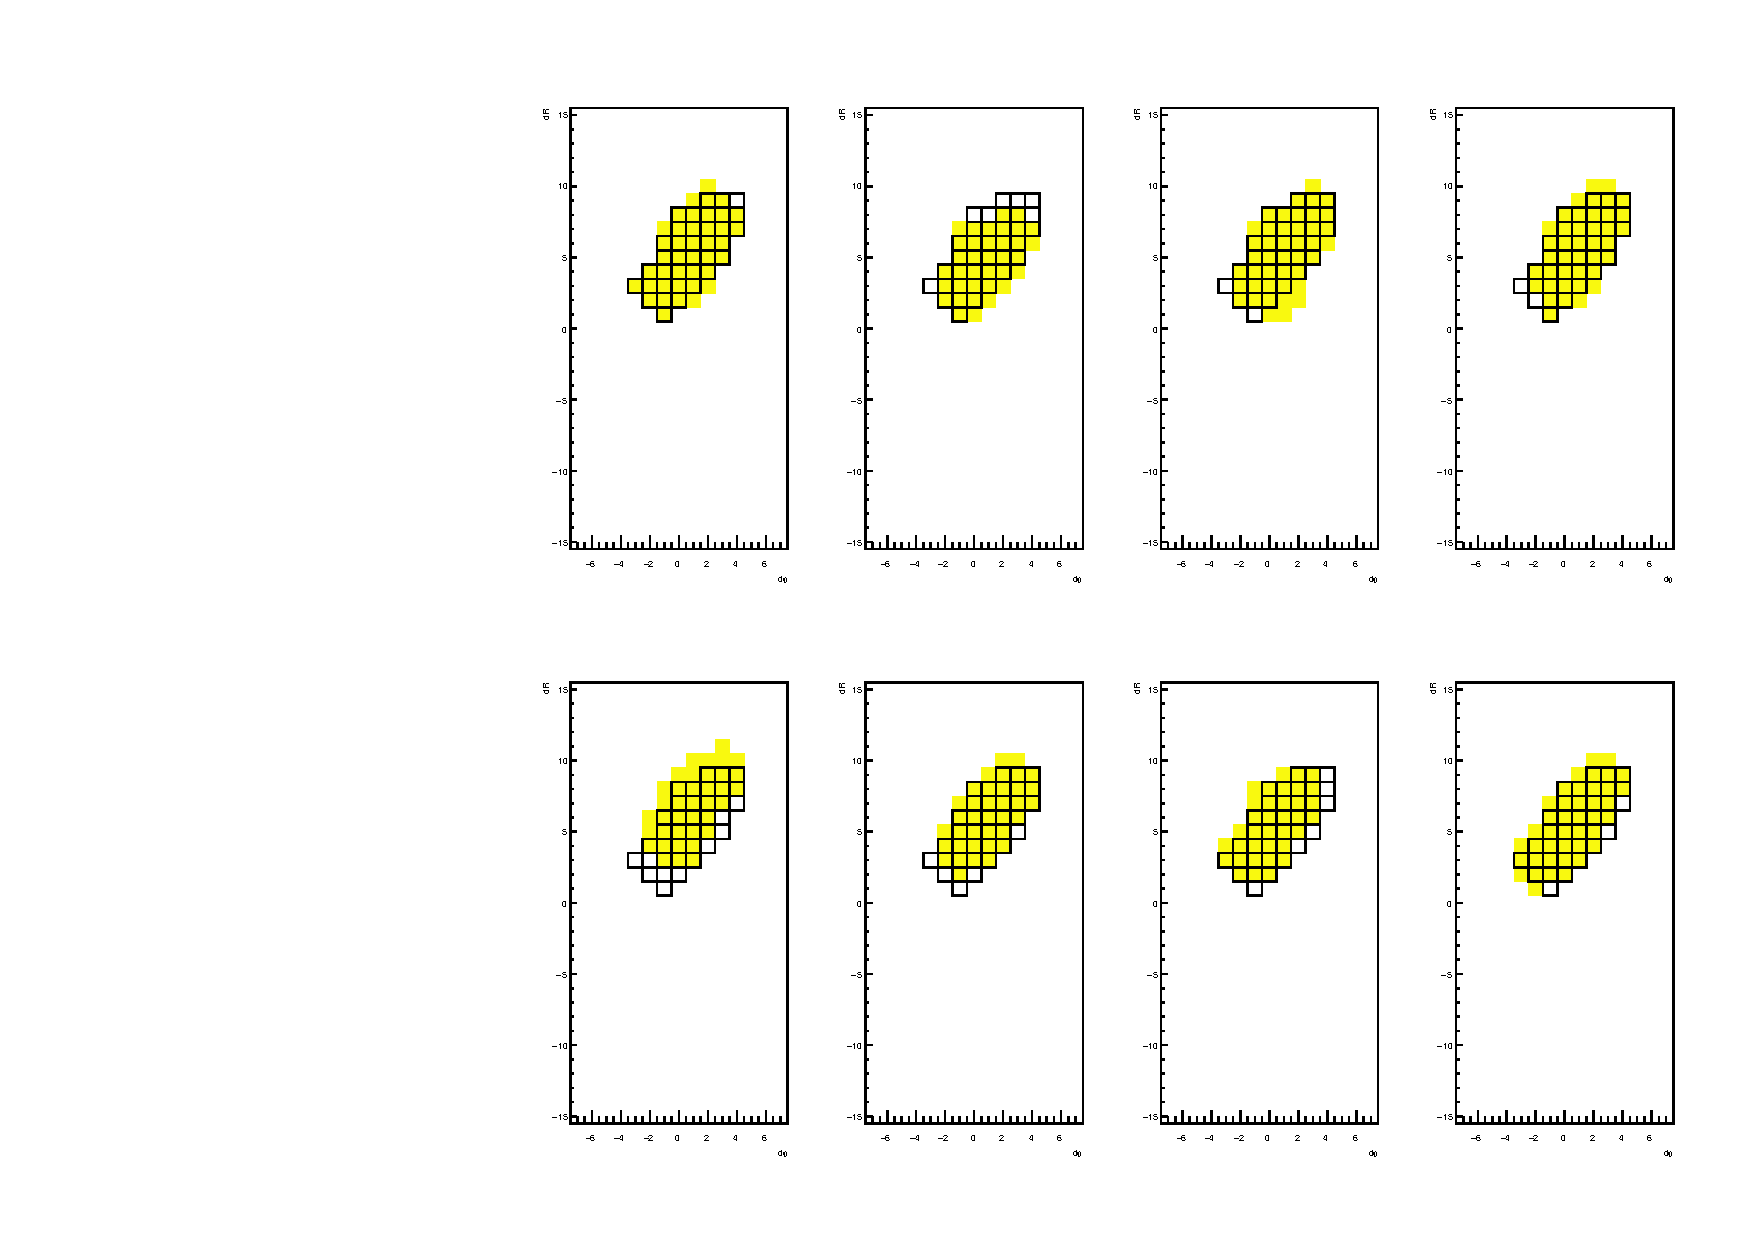
\includegraphics[clip, width=13cm]{fig/5/ALL_Aside_Endcap_phiSector_Octant1_roi58.pdf}
  \caption{$p_{\rm{T}}$閾値が14~GeVとなる領域の比較。黄色の領域が本手法で作成した$\mathrm{CW_{Data}}$、黒枠の領域が$\mathrm{CW_{2022}}$である。}
  \label{fig:CWv05v07}
\end{figure}

次に、2018年Run-2データを評価に用いた際の$\mathrm{CW_{Data}}$と$\mathrm{CW_{Simu}}$の比較を行う。図~\ref{fig:v06v07}に$p_{\rm{T}}$閾値14~GeVにおけるTurn-on curveを比較したプロットを示す。実際のデータに対して、$\mathrm{CW_{Data}}$を用いたトリガーの方がトリガー効率が良くなっているのが見て取れる。
\begin{figure}[tb]
  \centering
  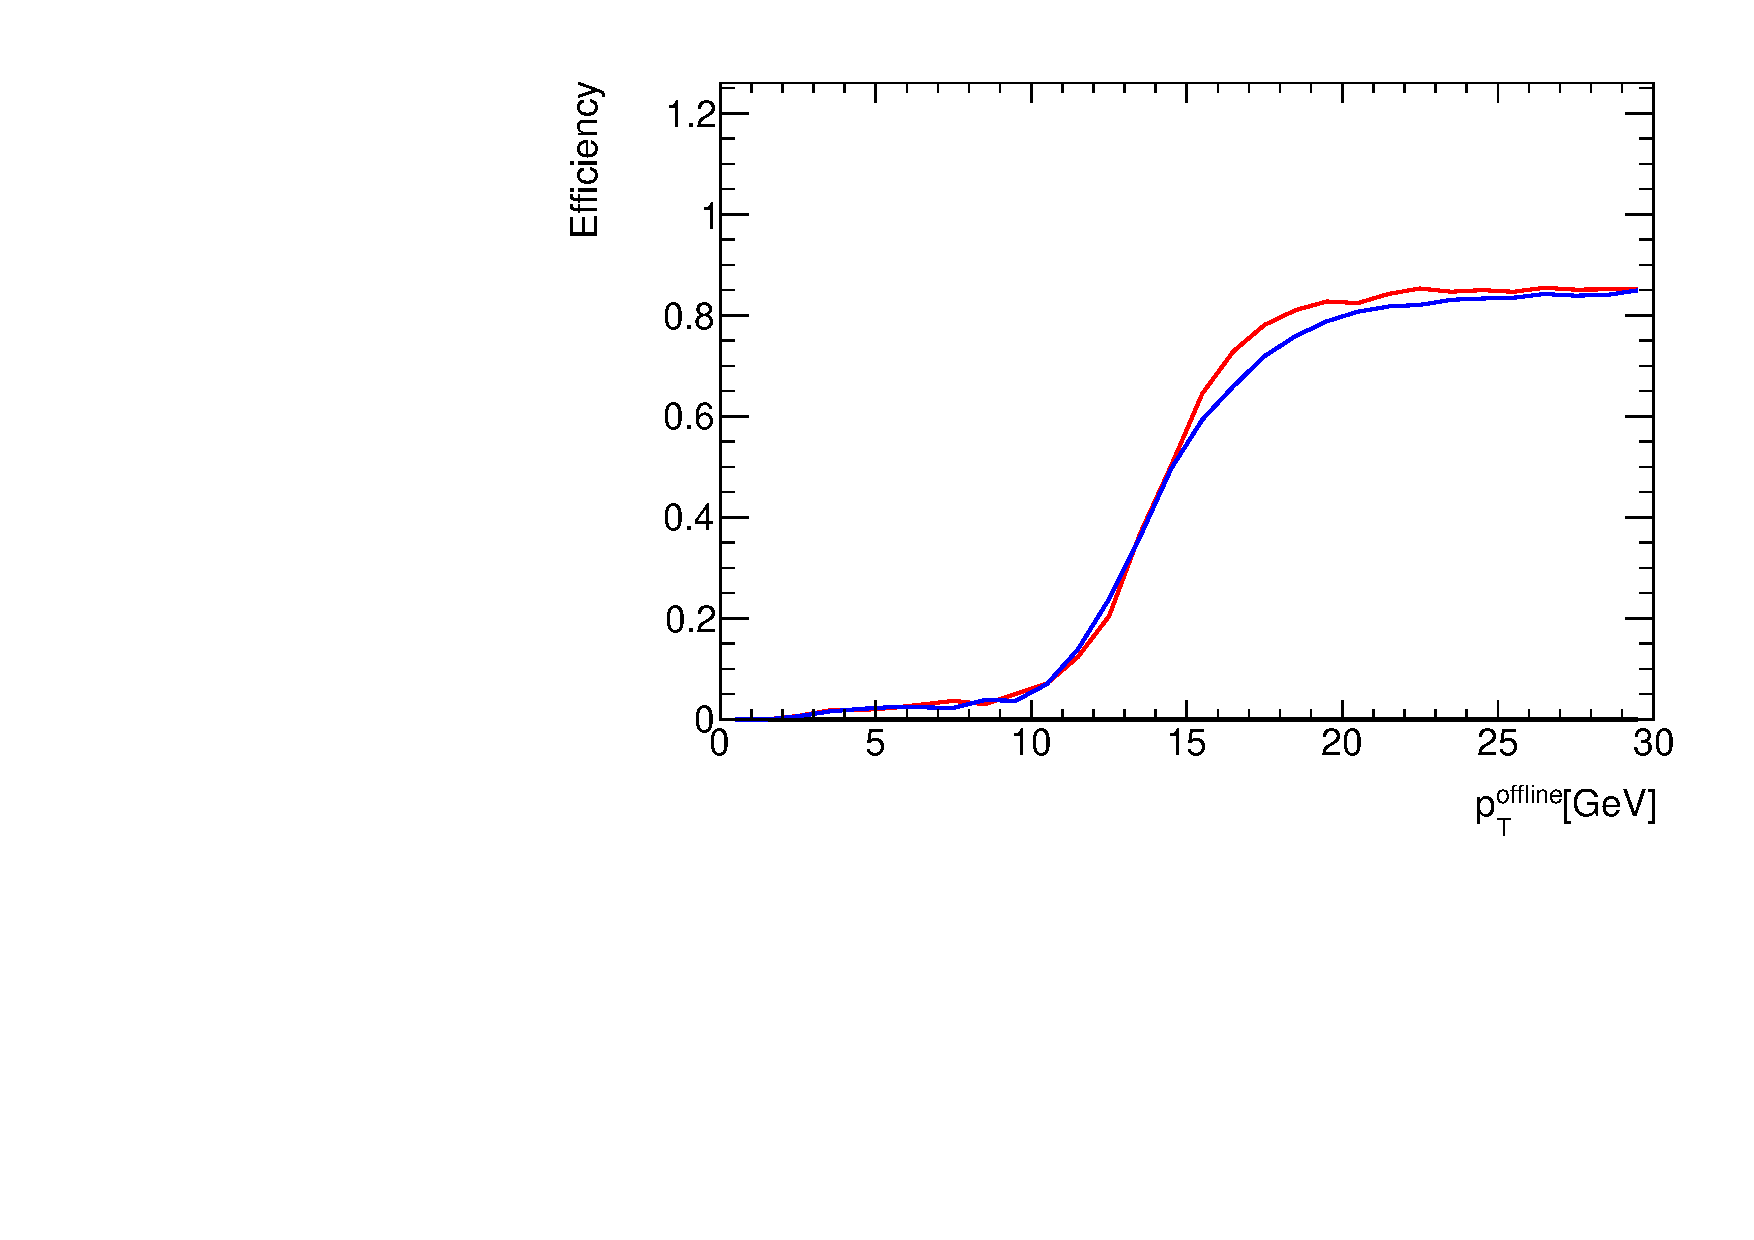
\includegraphics[clip, width=11cm]{fig/4/v06vsv07_MU14.pdf}
  \caption{$\mathrm{CW_{Data}}$と$\mathrm{CW_{Simu}}$のTurn-on curve。$p_{\rm{T}}$閾値14~GeVのトリガー効率の比較を行い、評価には2018年Run-2データを使用した。}
  \label{fig:v06v07}
\end{figure}

%\subsubsection{ミューオン電荷に対するトリガー性能の評価}
さらに、TGCチェンバーごとにミューオンの電荷別のトリガー効率の評価を行った。
あるTGCチェンバーにおける$\mathrm{CW_{Data}}$と$\mathrm{CW_{2022}}$の、ミューオンの電荷別に計算した$p_{\rm{T}}$閾値が14~GeVのトリガー効率を図~\ref{Eff_Chage}に示す。
磁場中のミューオンは電荷によって曲がる方向が違うため、検出器アライメントのズレによる影響を受けてCWもズレているとき、判定できる電荷に偏りが生じる。図~\ref{fig:v05_charge}に示すように、$\mathrm{CW_{2022}}$は検出器のズレに対する補正を行っていないために、ミューオンの電荷別に計算したトリガー効率に大きな差が出る。
一方、図~\ref{fig:v06_charge}に示すように、本研究の手法で作成した$\mathrm{CW_{Data}}$はCWが最適化されたことにより、電荷別に計算したトリガー効率がほとんど一致していることが見て取れる。
\begin{figure}
    %\centering
    \begin{tabular}{cc}
    \begin{minipage}[b]{0.45\hsize}
        %\centering
        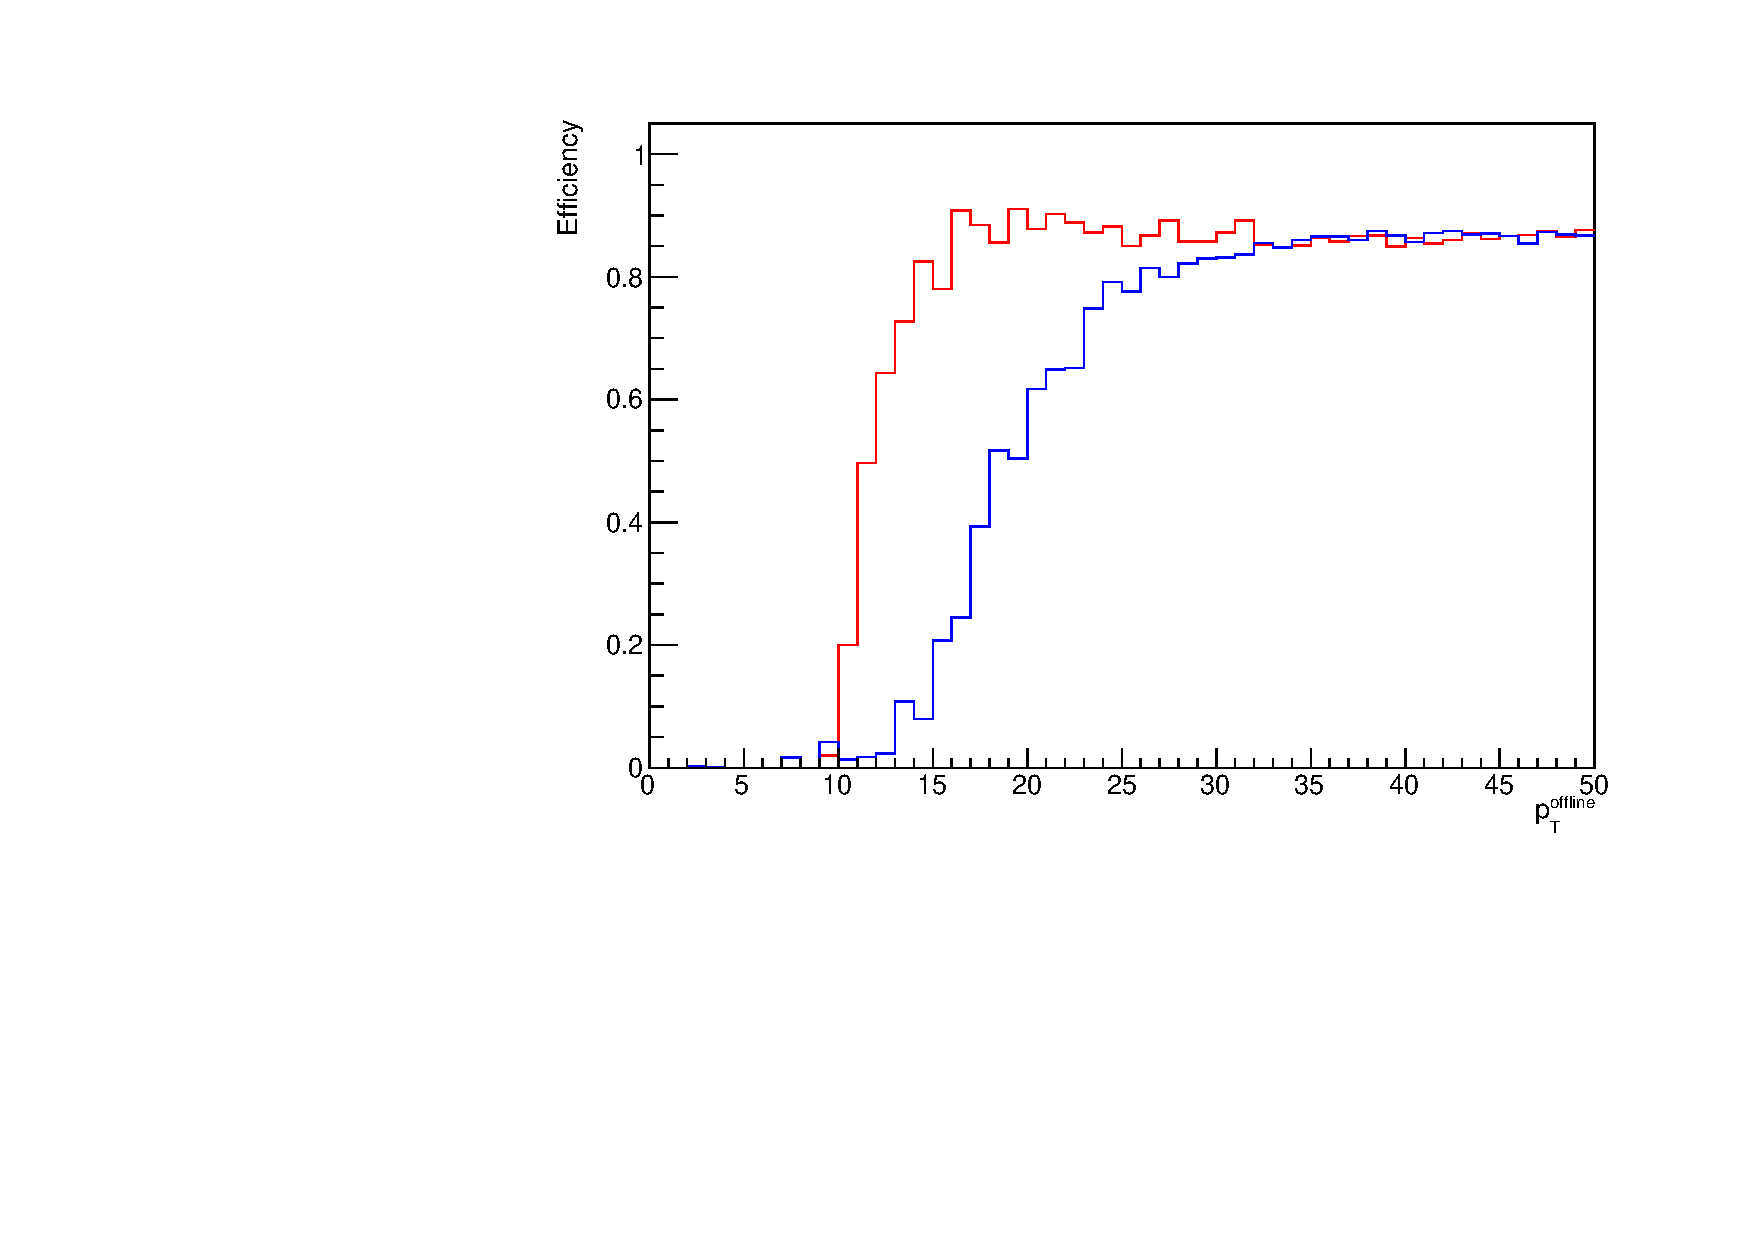
\includegraphics[clip, width=7cm]{fig/5/Eff_PNcharge_v05_phi0eta10.pdf}
        %\vspace{5pt}
        \subcaption{}
        \label{fig:v05_charge}
    \end{minipage}&
    %\hfill
    \begin{minipage}[b]{0.45\hsize}
        %\centering
        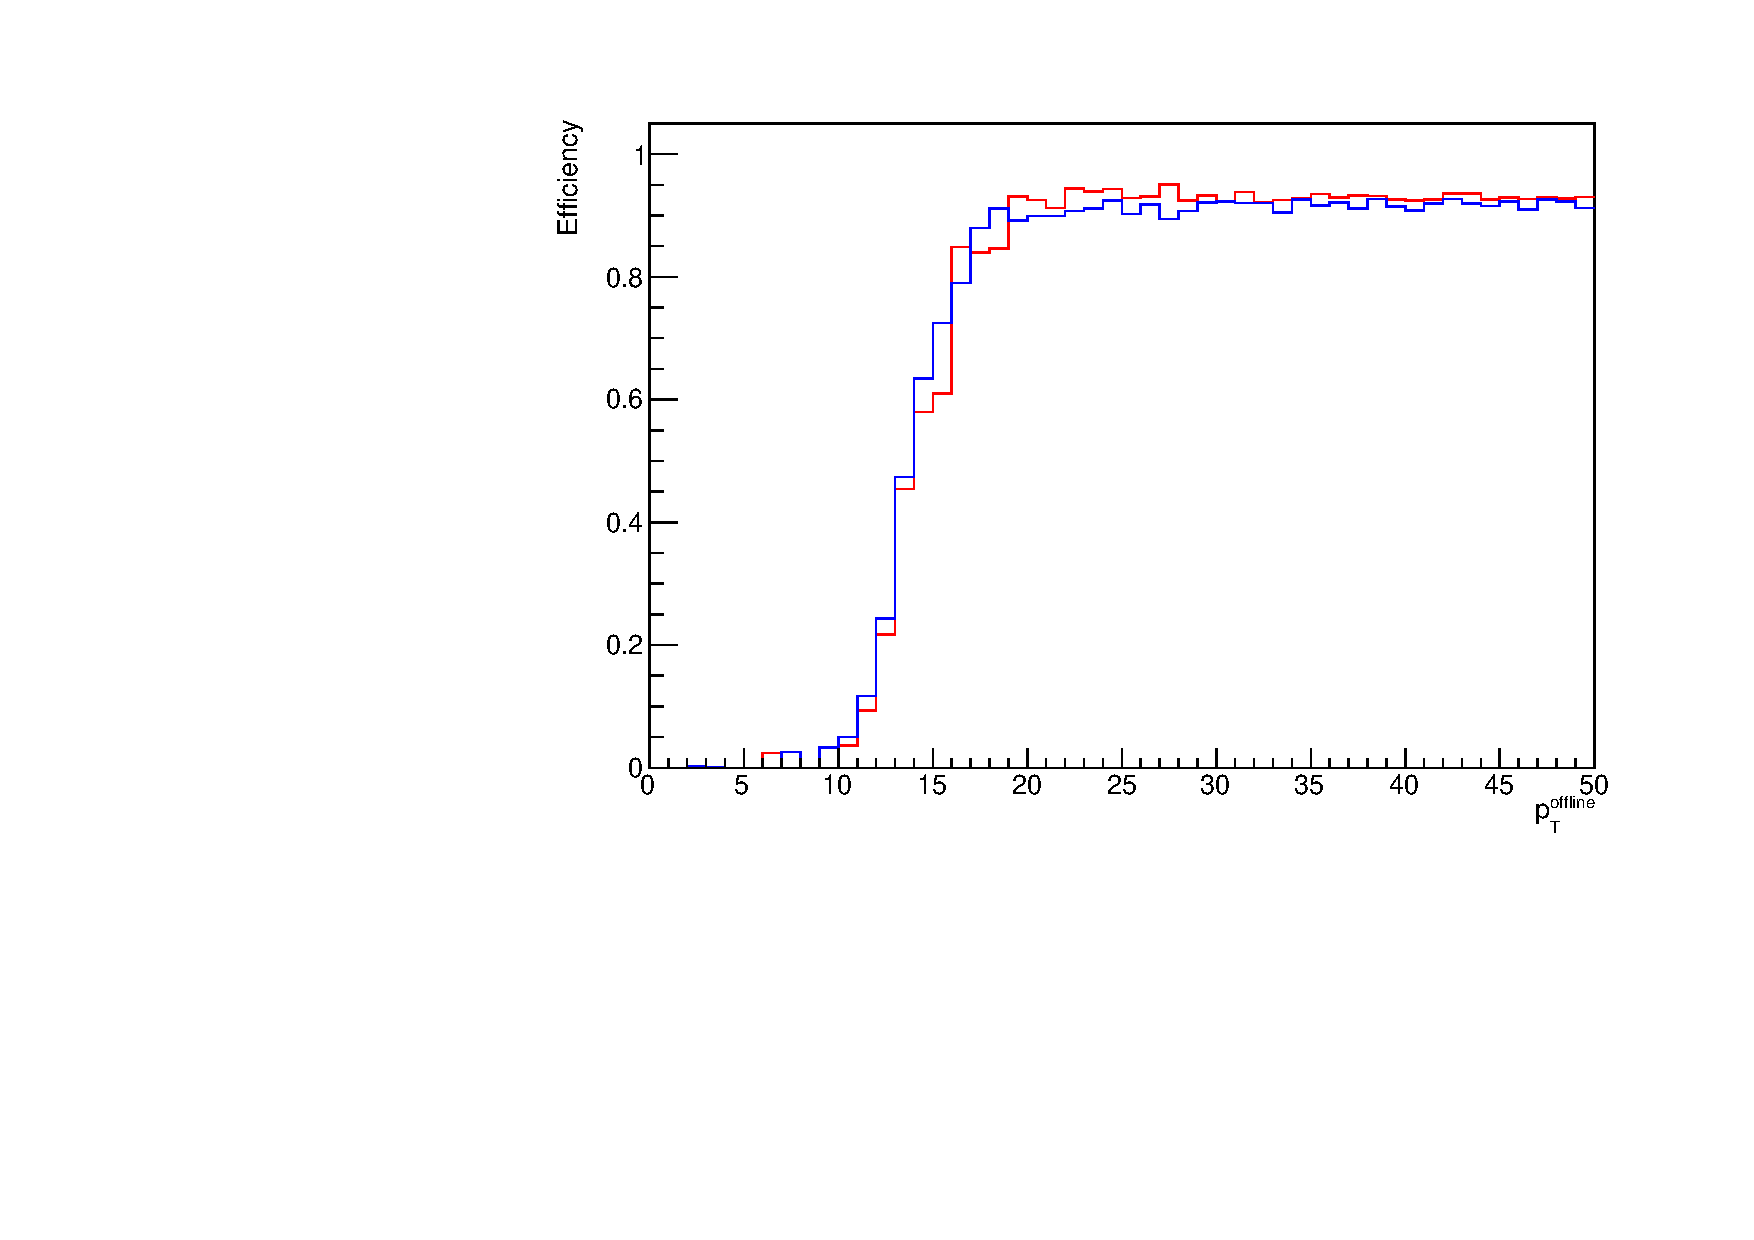
\includegraphics[clip, width=7cm]{fig/5/Eff_PNcharge_MLP_phi0eta10.pdf}
        %\vspace{5pt}
        \subcaption{}
        \label{fig:v06_charge}
    \end{minipage}
    \end{tabular}
    \caption{あるチェンバーにおける電荷別に計算した$p_{\rm{T}}$閾値14~GeVのTurn-on curveの比較。赤が正電荷、青が負電荷。(a):$\mathrm{CW_{2022}}$(b):$\mathrm{CW_{Data}}$}
    \label{Eff_Chage}
\end{figure}

本研究の手法では、実際のデータを機械学習のトレーニングに用いたことで、TGC 検出器の位置による磁場構造の違いや検出器のズレを自動で補正することができ、CWが最適化されたことを示している。




\subsection{トリガーレートの評価}
次に、本手法で作成したCWを使用したときのトリガーレートの評価を行う。トリガーレートとは、実験データにおけるトリガーが発行された事象数である。
2018年のRun-2データを用いてトリガーレートを計算する。
Run-2データにはHLTでのプリスケールによるバイアスが存在するため、バイアスのない状態でトリガーレートを計算するために、「HLT$\_$noalg$\_$L1MU4」を要求する。このトリガーはL1 TriggerにおいてpT閾値が4GeV以上を要求するが、HLTによる事象選別のない(Passthrough)トリガーチェインである。
その後、HLT$\_$noalg$\_$L1MU4が鳴ったイベントの中でL1$\_$MU$x$が鳴ったイベントがいくら存在するかを調べ、ルミノシティが$2\times10^{43}$~cm$^{-2}$s$^{-1}$の時のL1$\_$MU4のトリガーレート(3400kHz)をかけることでMUxのトリガーレートを見積もる。式~\eqref{equ:トリガーレート}にトリガーレートの計算式を示す。
\begin{equation}
    \rm{MU}xのレート[\rm{kHz}] = \frac{\rm{MU}xが鳴ったイベント数}{HLT\_noalg\_L1MU4が鳴った全イベント数}\times L1\_MU4のレート[kHz]
    \label{equ:トリガーレート}
\end{equation}
図~\ref{fig:Ratev05v06}に2016年で取得されたデータを用いて算出したトリガーレートを示す。

\begin{figure}[tb]
  \centering
  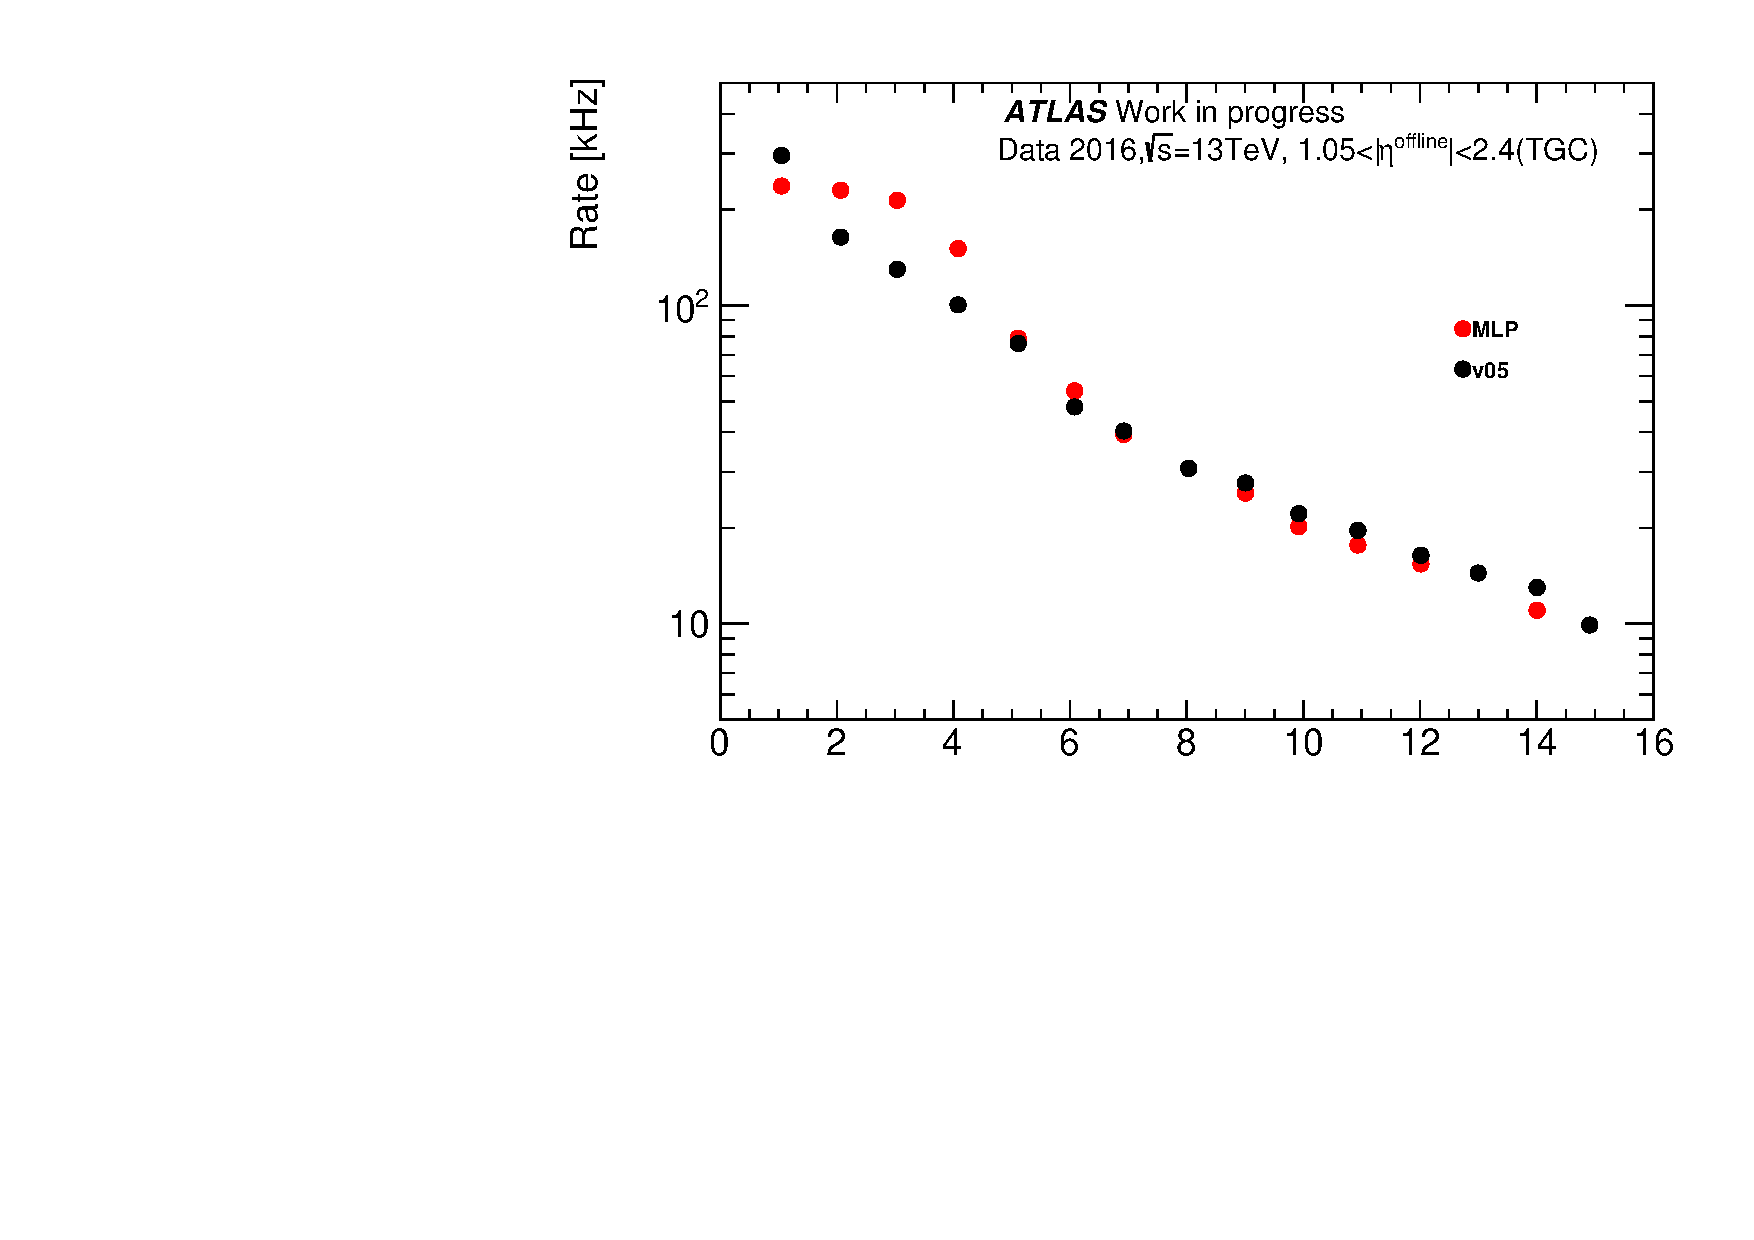
\includegraphics[clip, width=11cm]{fig/5/15rate.pdf}
  \caption{TGCにおけるシングルミューオンのトリガーレート。}
  \label{fig:Ratev05v06}
\end{figure}
プライマリートリガーである$p_{\rm{T}}$閾値14~GeVのトリガーレートは、本研究の手法で作成した$\mathrm{CW_{Data}}$では15~kHz、2022年度Run-2で使用された$\mathrm{CW_{2022}}$では16~kHzとなり、トリガーレートの削減が確認できた。また、$p_{\rm{T}}$閾値7~GeV以上のトリガーにおいて、$\mathrm{CW_{Data}}$のトリガーレートの値は$\mathrm{CW_{2022}}$と同等であることが見て取れる。
しかし、$p_{\rm{T}}$閾値4~GeV、5~GeV、6~GeVのトリガーに関してはトリガーレートの増加が見られた。
これは、\ref{fig:Effictive_thr_v1}で示したように、低いEffective Threshouldへの変換ができていなことが原因で、低い$p_{\rm{T}}$閾値のトリガーの性能が悪くなってしまったと思われる。
ただし、Run-3以降のエンドキャップ部のミューオントリガーでは\ref{section2-2-4}節で述べたようにNSWによるインナーコインシデンスを行うことで、トリガーレートの大幅な削減が見込まれている。
また、本研究で開発した手法では、$p_{\rm{T}}$閾値を柔軟に選択することができるため、トリガーレートの削減に焦点を置いた$p_{\rm{T}}$閾値の選択をすることでトリガーレートを抑えることのできるCWを作成可能である。



\subsection{本章のまとめ}
本章では作成したCWの評価を行った。
15段階のトリガー効率の評価を、Turn-on CurveのPlateau EfficiencyとResolutionといった観点から評価を行った。
本研究の手法で作成した2種類のCWは$\mathrm{CW_{2022}}$のTurn-on Curveと比べ、Plateau Efficiencyが高く、立ち上がりが鋭くなったことから、トリガー効率の向上が確認できた。
また、L1Muonのプライマリートリガーである$p_{\rm{T}}$閾値14~GeVのトリガー効率について、図~\ref{EffMU14}にTGCのRoIにおける$p_{\rm{T}}$閾値14~GeVのトリガー効率を示す。$\mathrm{CW_{2022}}$はトリガー効率が85.4$\%$であったのに対し、$\mathrm{CW_{Data}}$ではトリガー効率が86.7$\%$となったことから約1$\%$の向上が見込まれる。

\begin{figure}
    %\centering
    \begin{tabular}{cc}
    \begin{minipage}[b]{0.45\hsize}%
        %\centering
        \hspace*{-1cm}
        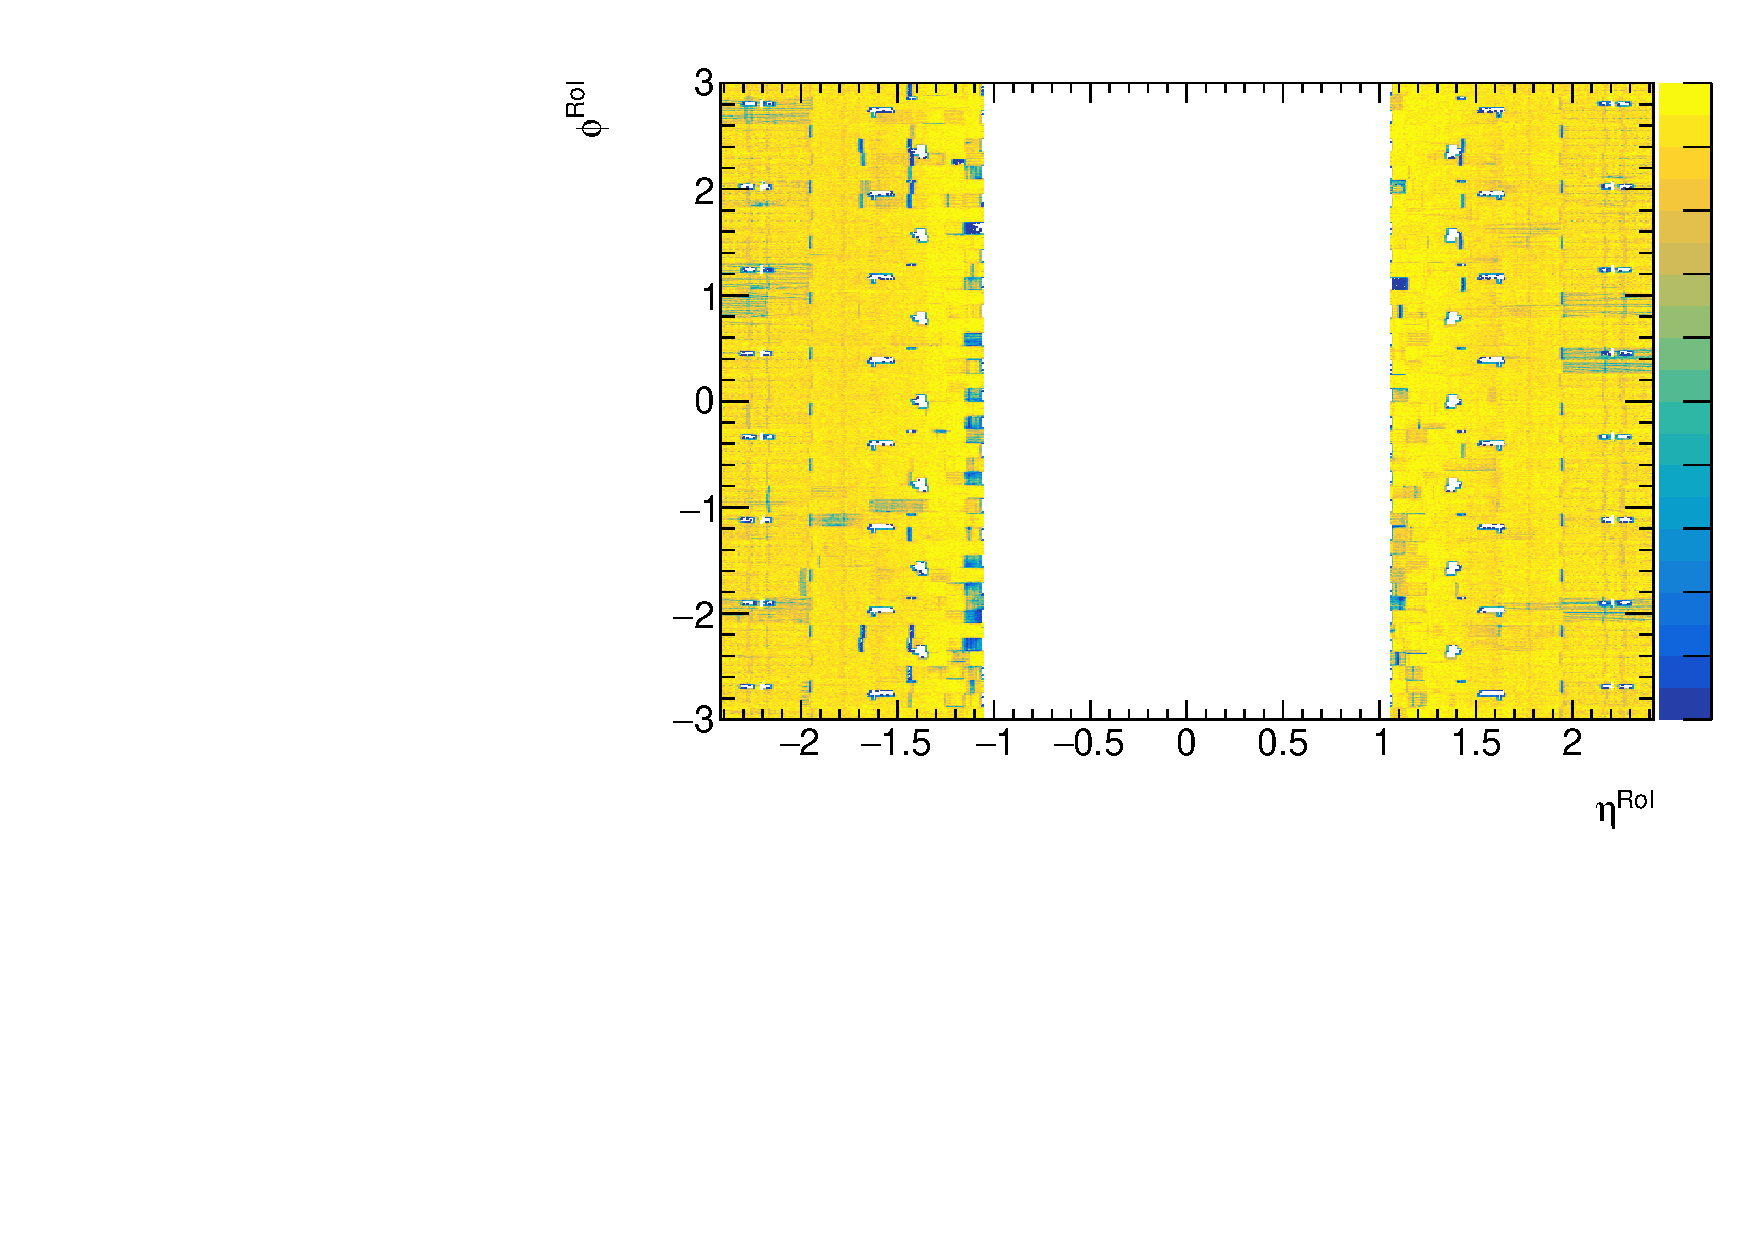
\includegraphics[clip, width=7cm]{fig/5/h2_Data14_Eff.pdf}
        %\vspace{5pt}
        \subcaption{}
        \label{fig:dataEffMU14}
    \end{minipage}%
    %\hfill
    \begin{minipage}[b]{0.55\hsize}%
        %\centering
        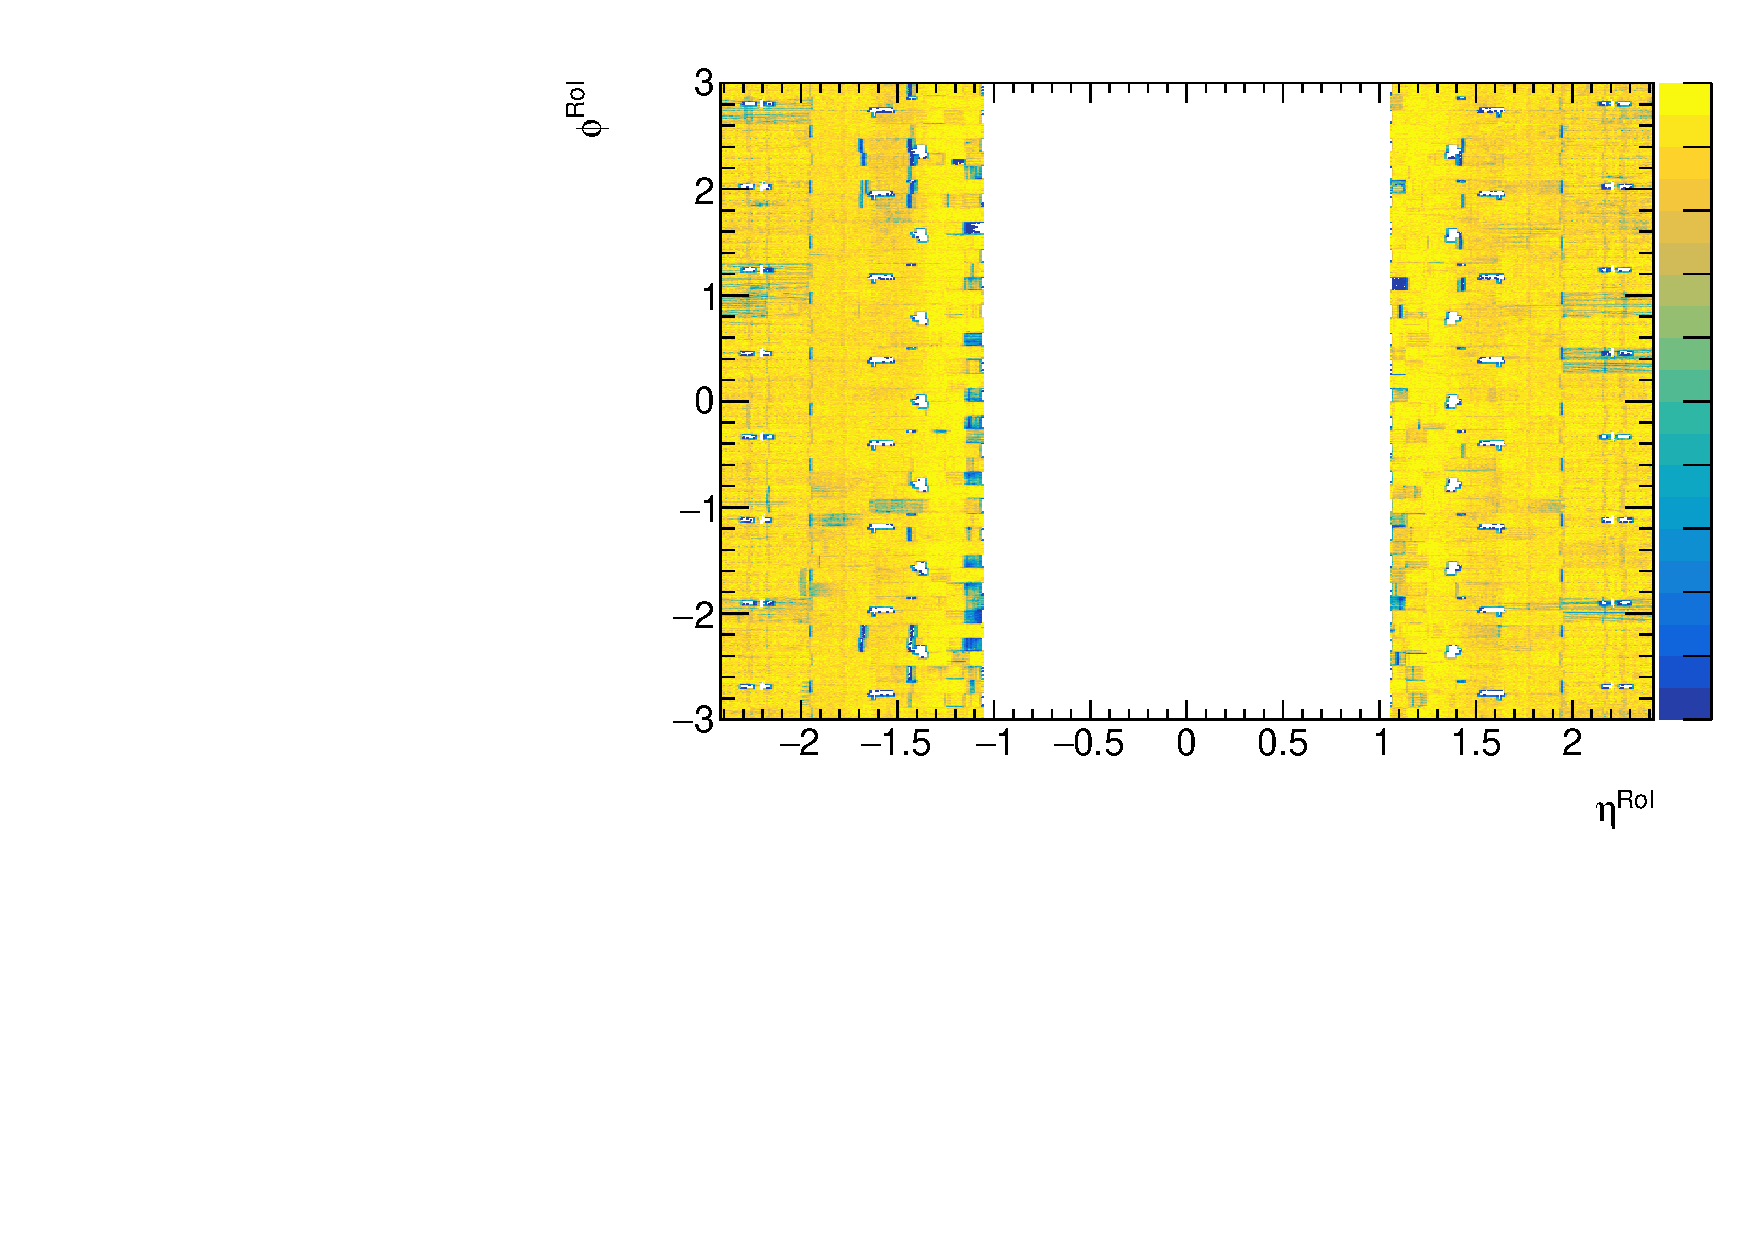
\includegraphics[clip, width=7cm]{fig/5/h2_v0514_Eff.pdf}
        %\vspace{5pt}
        \subcaption{}
        \label{fig:v05EffMU14}
    \end{minipage}%
    \end{tabular}
    \caption{TGCのRoIにおけるトリガー効率。分母を$p_{\rm{T}}$が20~GeV以上のオフライン再構成されたミューオンとし、その中で$p_{\rm{T}}$閾値14~GeVのトリガーを鳴らしたミューオンの割合を表している。(a):$\mathrm{CW_{Data}}$(b):$\mathrm{CW_{2022}}$}
    \label{EffMU14}
\end{figure}

さらに、$p_{\rm{T}}$分解能の評価を$p_{\rm{T}}$ residualを計算することで評価を行った。
本研究の手法で作成したCWは、2022年度Run-2で使用された$\mathrm{CW_{2022}}$と比べて$p_{\rm{T}}^{offline}$分解能のmean値が悪くなっているが、Resolutionを比べると改善されていることから、機械学習の出力からの$p_{\rm{T}}$閾値の選択方法を変更することによってmean値においても改善が見込まれる。

また、本研究の手法で期待される機械学習による最適化の評価を行った。
また、ミューオンの電荷別にトリガー効率を見たところ、電荷によるトリガー効率の依存性がほとんど見られなくなった。
このことから、検出器アライメントのズレに対する補正が行えることが確認できた。

トリガーレートに関しての評価も行った。
プライマリートリガーである$p_{\rm{T}}$閾値14~GeVのトリガーレートは、本研究の手法で作成した$\mathrm{CW_{Data}}$では15~kHz、2022年度Run-2で使用された$\mathrm{CW_{2022}}$では16~kHzとなり、トリガーレートの削減が確認できた。また、$p_{\rm{T}}$閾値7~GeV以上のトリガーにおいて、$\mathrm{CW_{Data}}$のトリガーレートの値は$\mathrm{CW_{2022}}$と同等であることが見て取れる。


%低い$p_{\rm{T}}$閾値のトリガーに対しての課題があるが、トレーニングデータの低い$p_{\rm{T}}$のミューオン数を増加させることや、適切な重みをつけてトレーニングを行うことで、
